\clearpage
\section{Object definition and selection}
\label{sec:object-selection}

The signal signature was studied in Section~\ref{sec:signal-signature}. In this section, a set of object selection criteria is devised to obtain a sample that is as pure as possible with respect to the signal leptons, while still retaining as much signal as possible. As discussed in Section~\ref{sec:search-strategy}, the focus is on selecting opposite-charge, same-flavor leptons \ellell resulting from the \neutt that decays into a \neuto and a \PZstar, \ie, \neuttdecay. Two choices of $\dmo$ are presented in the following section: a relatively high $\dmo$ of $\dmo=5.63\GeV$ and a low $\dmo$ of $\dmo=1.92\GeV$, but not so low as to prevent enough electrons from surviving the initial reconstruction \pt threshold of $5\GeV$. The higgsino parameter is fixed at $\mu=100\GeV$.

In Section~\ref{sec:signal-signature}, the base selection required at least one jet in the event with $\pt \geq 30\GeV$ and $\abs{\eta}<2.4$, without any other selection. However, unlike in that section, objects are not weighted to any luminosity in this section, as the focus is on the proportion between object types. Two types of reconstructed leptons are differentiated: those originating from the targeted decay \neuttdecay, shown in blue, and those that do not, referred to as \emph{other}, shown in yellow. Signal leptons are marked as such by matching a reconstructed lepton to a generator level lepton, which has been confirmed to have the \neutt as its parent. Leptons marked as \emph{other} may have been misreconstructed, misidentified, or may be a result of the hadronisation process in a jet (such as the \gls{isr} jet).

In the following sections, the term \emph{efficiency} refers to the proportion of signal leptons passing a selection, divided by the initial number of signal leptons, and the term \emph{purity} refers to the proportion of signal leptons (blue) to the sum of the signal leptons and \emph{other} leptons (yellow). The goal is to find selection criteria with high efficiency and high purity. However, these two quantities can sometimes compete with each other, requiring compromises.

\subsection{Electrons}
\label{sec:object-selection-electrons}
%\subsubsection{Signal electron selection}

The electrons are subject to an initial lower threshold on the reconstructed \pt of $5\GeV$, and are reconstructed using a loose \gls{wp}. The first distribution of interest regarding the electrons is their angular separation from the leading jet in the event, denoted as $\DR(\jmath_1,\Pe)$. The distributions are shown in Figure~\ref{fig:electrons-dr-lj}. The signal electrons are predominantly located outside the leading jet. This is because the leading jet is typically an \gls{isr} jet, which boosts the \tchiz system away from it, causing them to be back-to-back. Thus, a cut of $\DR(\jmath_1,\Pe)>0.4$ is made to account for this. Furthermore, as already discussed in Section~\ref{sec:signal-signature}, probing lower $\dm$ necessitates access to low $\pt$ leptons. The threshold of $\pt\geq 5\GeV$ on the electrons leads to reduced signal acceptance. This is evident from the difference between the high and low $\dm$ cases.

\begin{figure}[p]
\centering
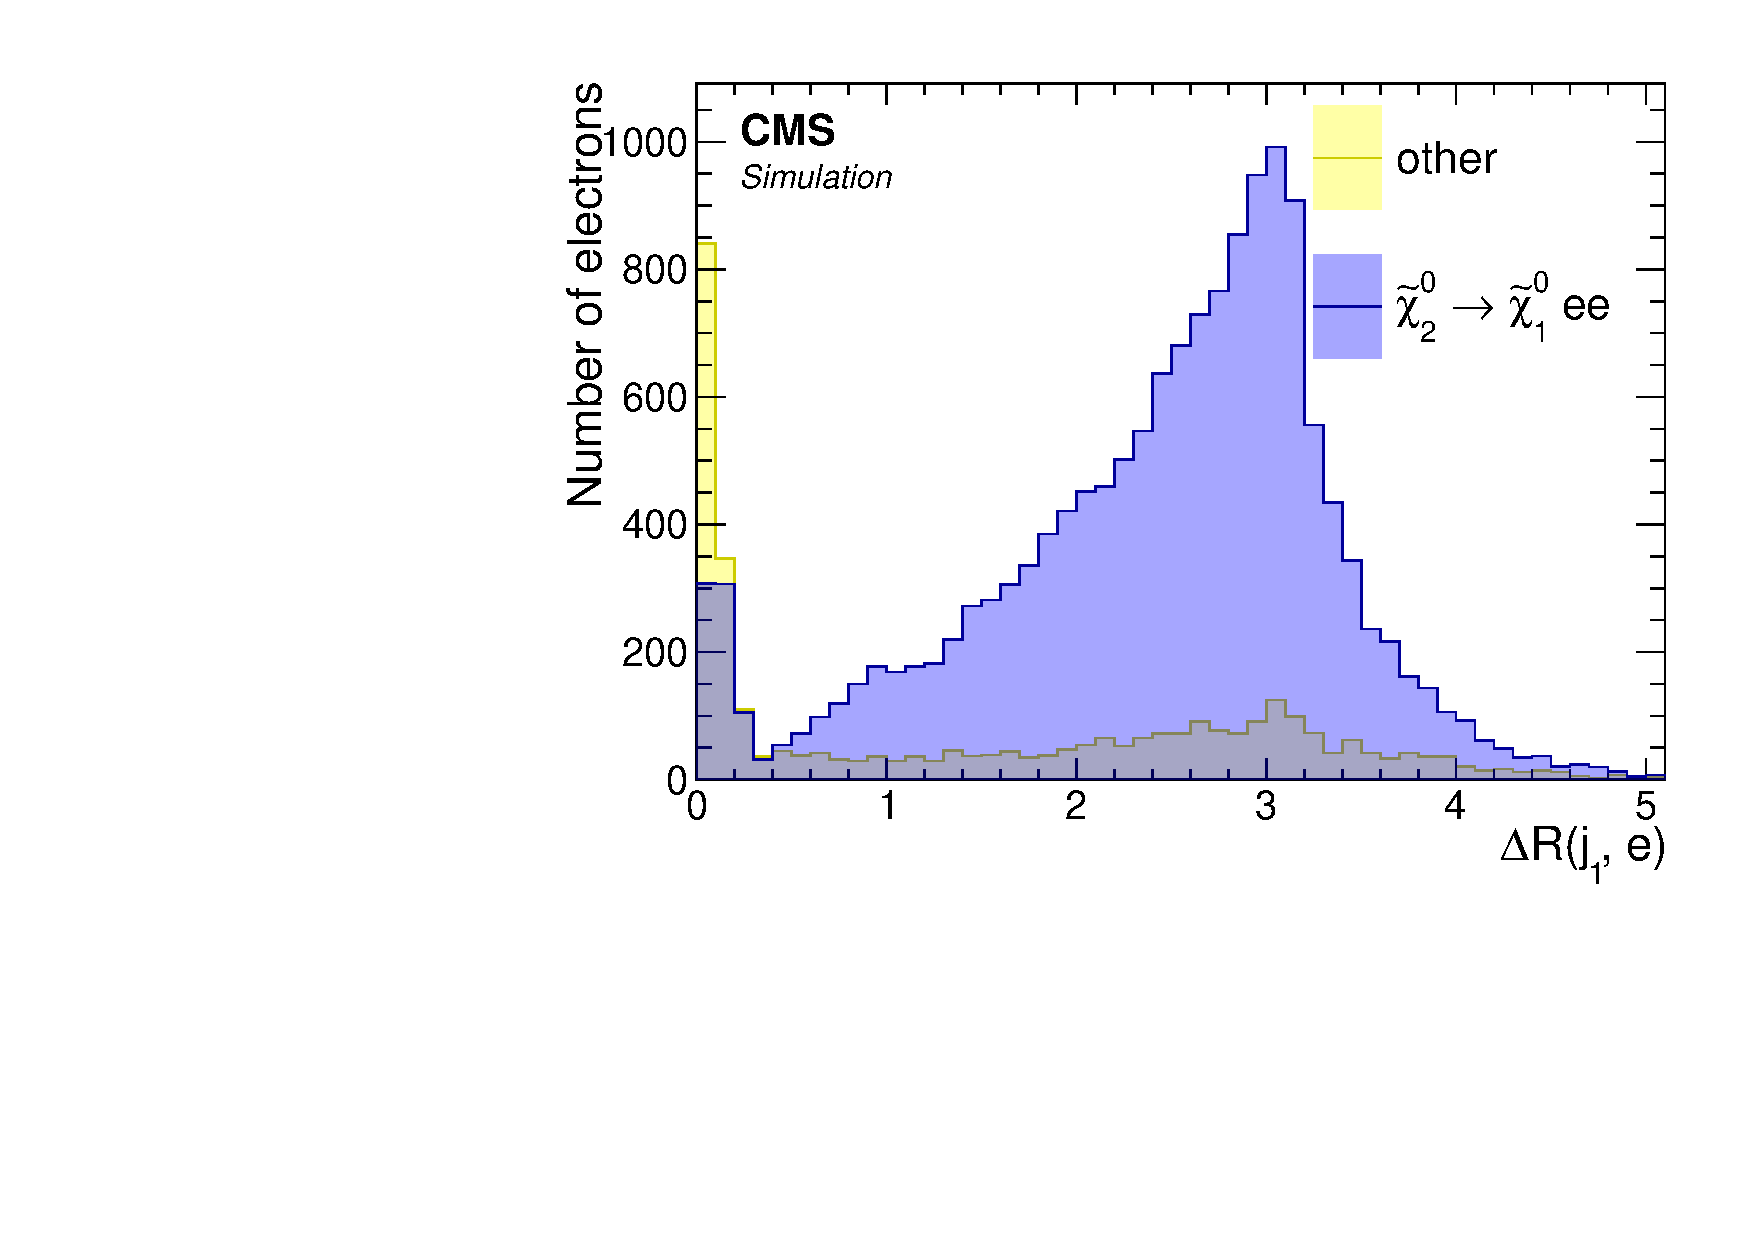
\includegraphics[width=0.48\linewidth]{plots/lepton_selection/lepton_selection_dm5p63/none_Electrons_rlj.pdf} \,
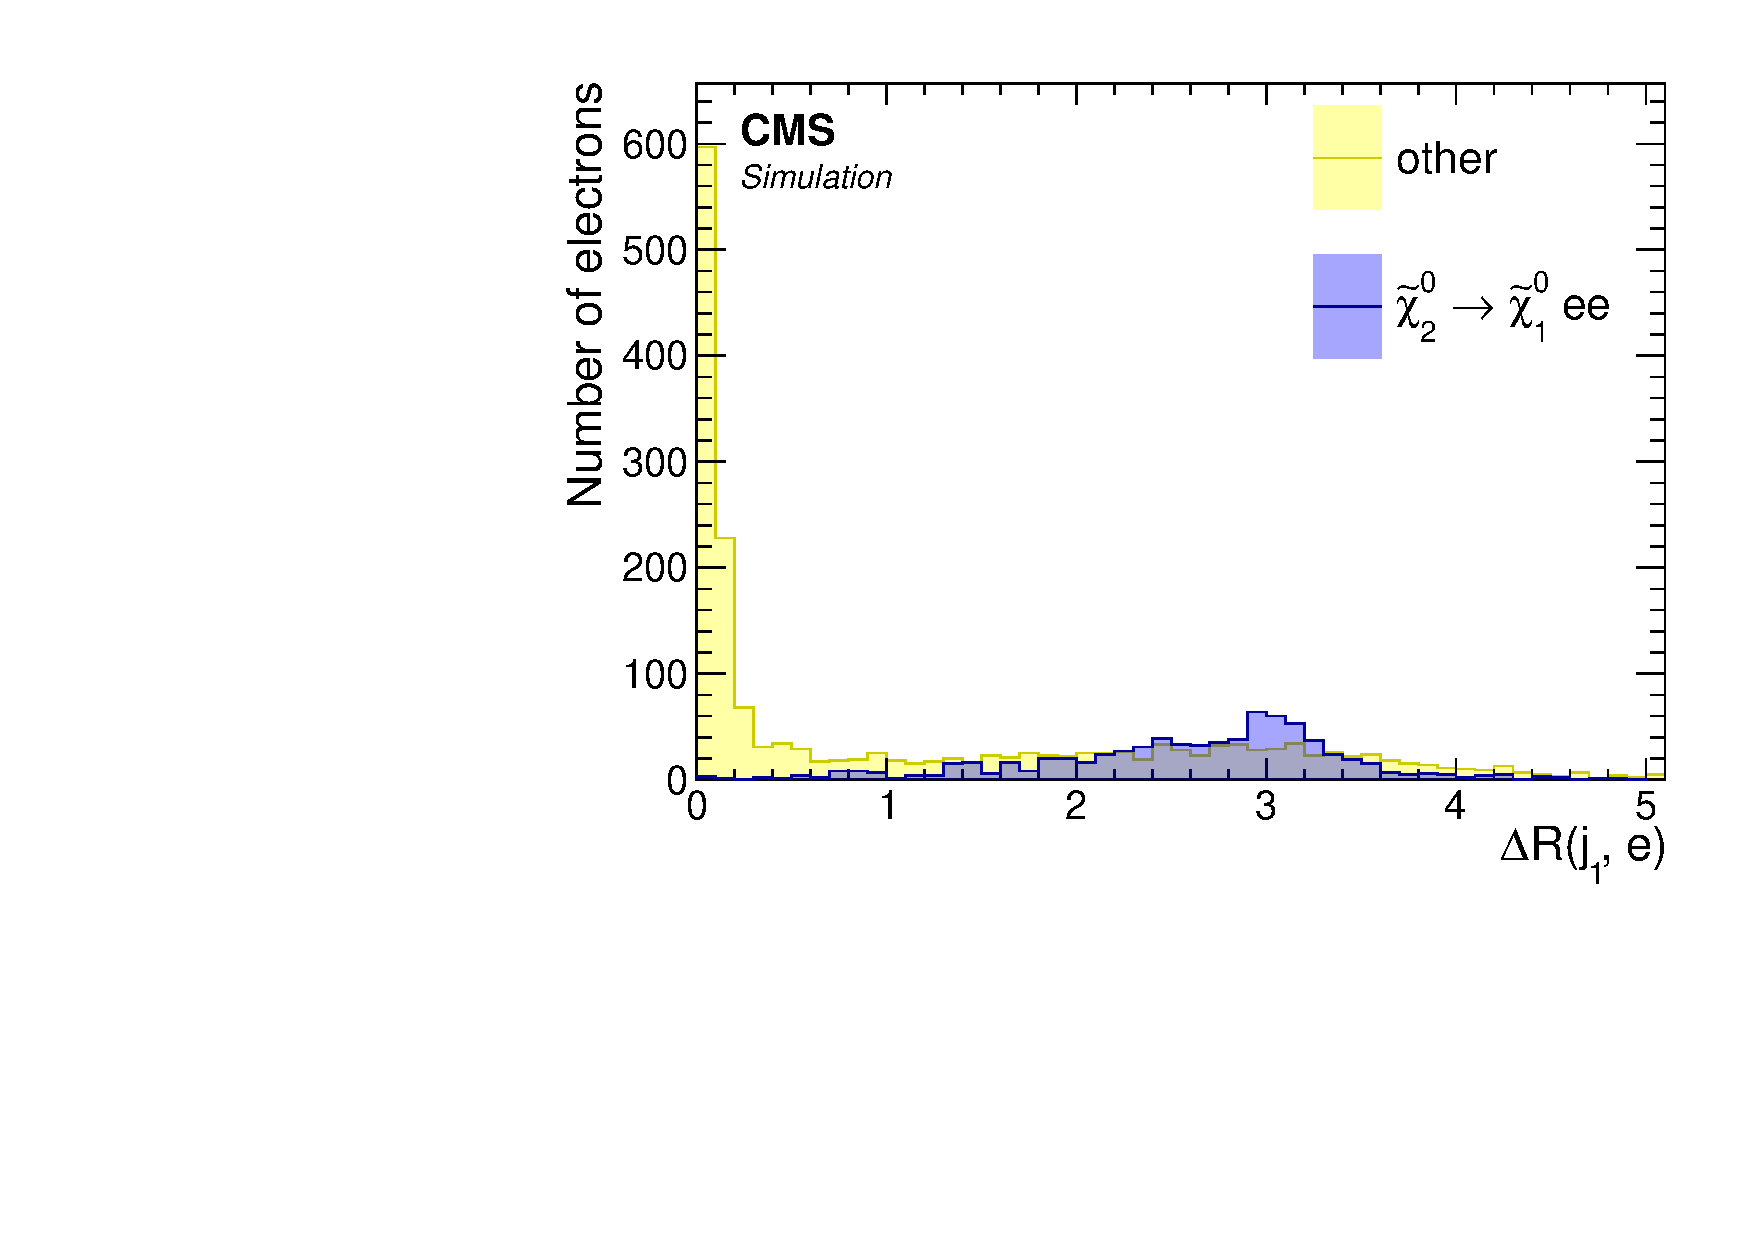
\includegraphics[width=0.48\linewidth]{plots/lepton_selection/lepton_selection_dm1p92/none_Electrons_rlj.pdf}  \\
\caption[Angular seperation between reconstructed electrons and the leading jet $\DR(\jmath_1,\Pe)$]{Angular separation between reconstructed electrons with loose ID and the leading jet $\DR(\jmath_1,\Pe)$ for $\dm=5.63\GeV$ (left) and $\dm=1.92\GeV$ (right).}
\label{fig:electrons-dr-lj}
\end{figure}

Distributions of electron $\pt$ are examined by applying the $\DR(\jmath_1,\Pe)>0.4$ cut. It is observed that the $\pt$ distribution depends strongly on the $\dm$, as previously seen for muons in Section~\ref{sec:muon-eta-pt}. Thus, a choice must be made regarding which $\dm$ to prioritize, and the lower $\dm$ case is chosen for increased sensitivity. As can be seen in  expected Figure~\ref{fig:electrons-selection-pt}, the $\pt$ distribution of the electrons falls more rapidly for the low \dm case. It is observed that there are very few electrons with \pt above $15\GeV$. Therefore, a cut of $\pt<15\GeV$ is chosen. The $\eta$ distribution is seen in Figure~\ref{fig:electrons-selection-eta}, after the previous cuts to gain a better understanding of where most of the non-signal electrons originate from. For the $\dm=1.92\GeV$ case, it can be clearly seen that the endcaps of the \gls{ecal} are performing worse compared to the barrel ($\abs{\eta}<1.48$). The transition is easily noticeable through a sharp drop in purity at the transition. This effect is most pronounced for low-$\pt$ electrons.

\begin{figure}[p]
\centering
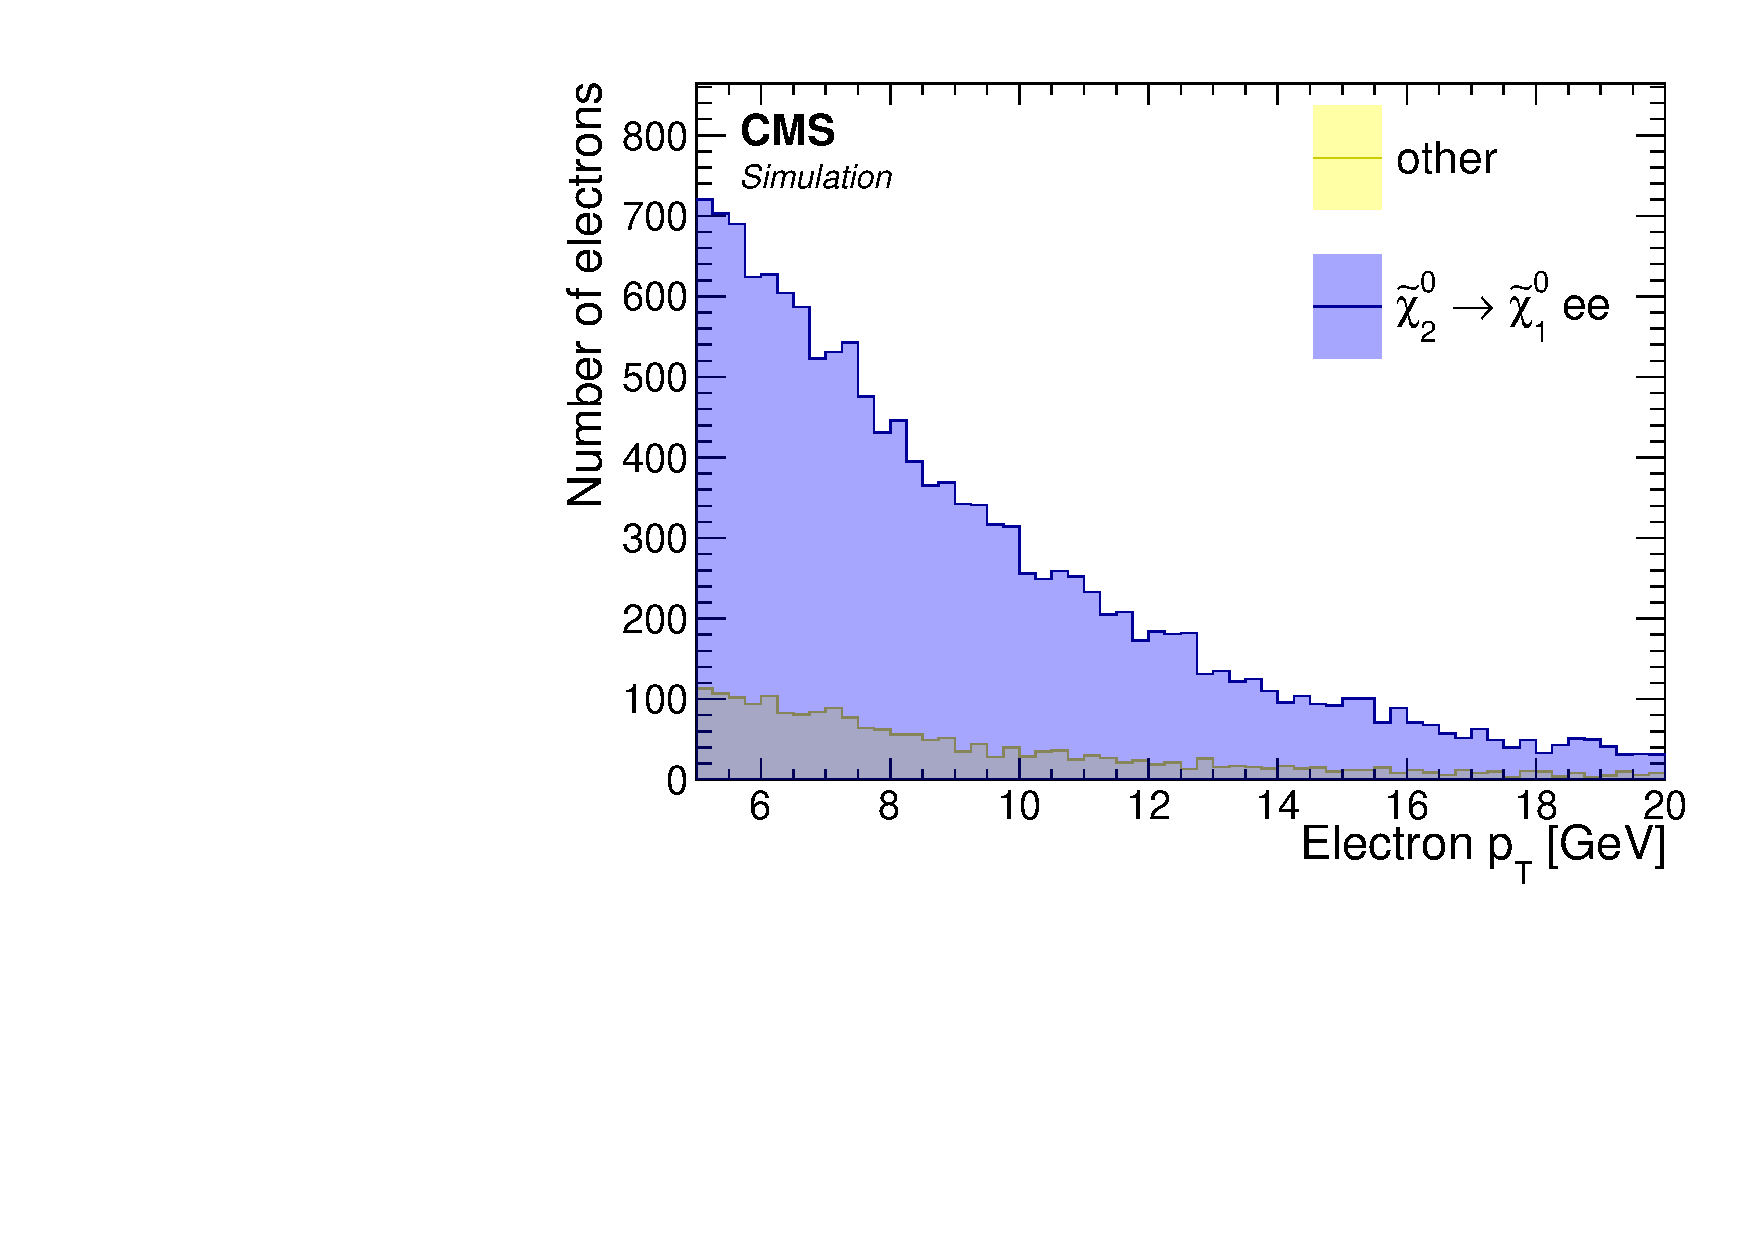
\includegraphics[width=0.48\linewidth]{plots/lepton_selection/lepton_selection_dm5p63/none_Electrons_pt.pdf} \,
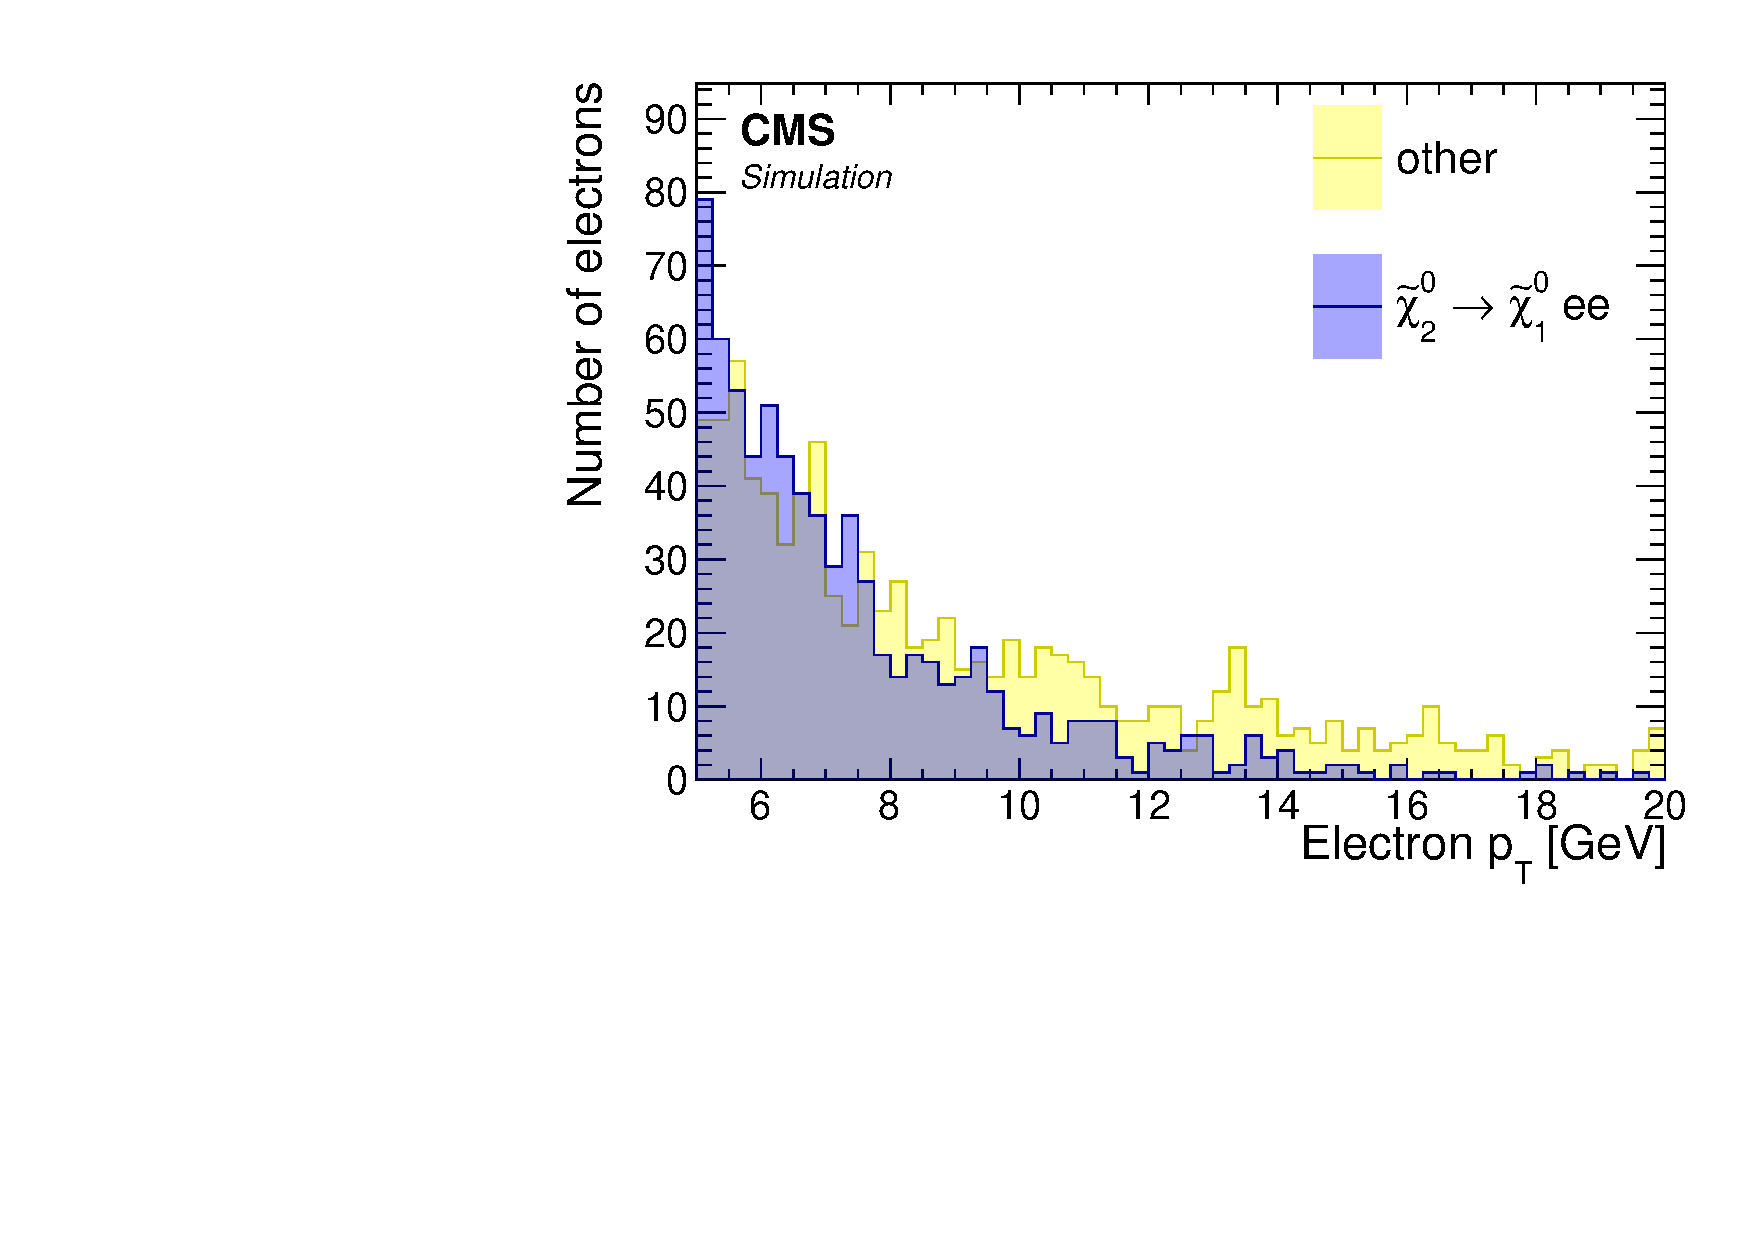
\includegraphics[width=0.48\linewidth]{plots/lepton_selection/lepton_selection_dm1p92/none_Electrons_pt.pdf}  \\
\caption[Distribution of reconstructed electron $\pt$ with loose ID]{Distribution of reconstructed electron $\pt$ with loose ID for $\dm=5.63\GeV$ (left) and $\dm=1.92\GeV$ (right). A cut of $\DR(\jmath_1,\Pe)>0.4$ is applied. }
\label{fig:electrons-selection-pt}
\end{figure}

\begin{figure}[p]
\centering
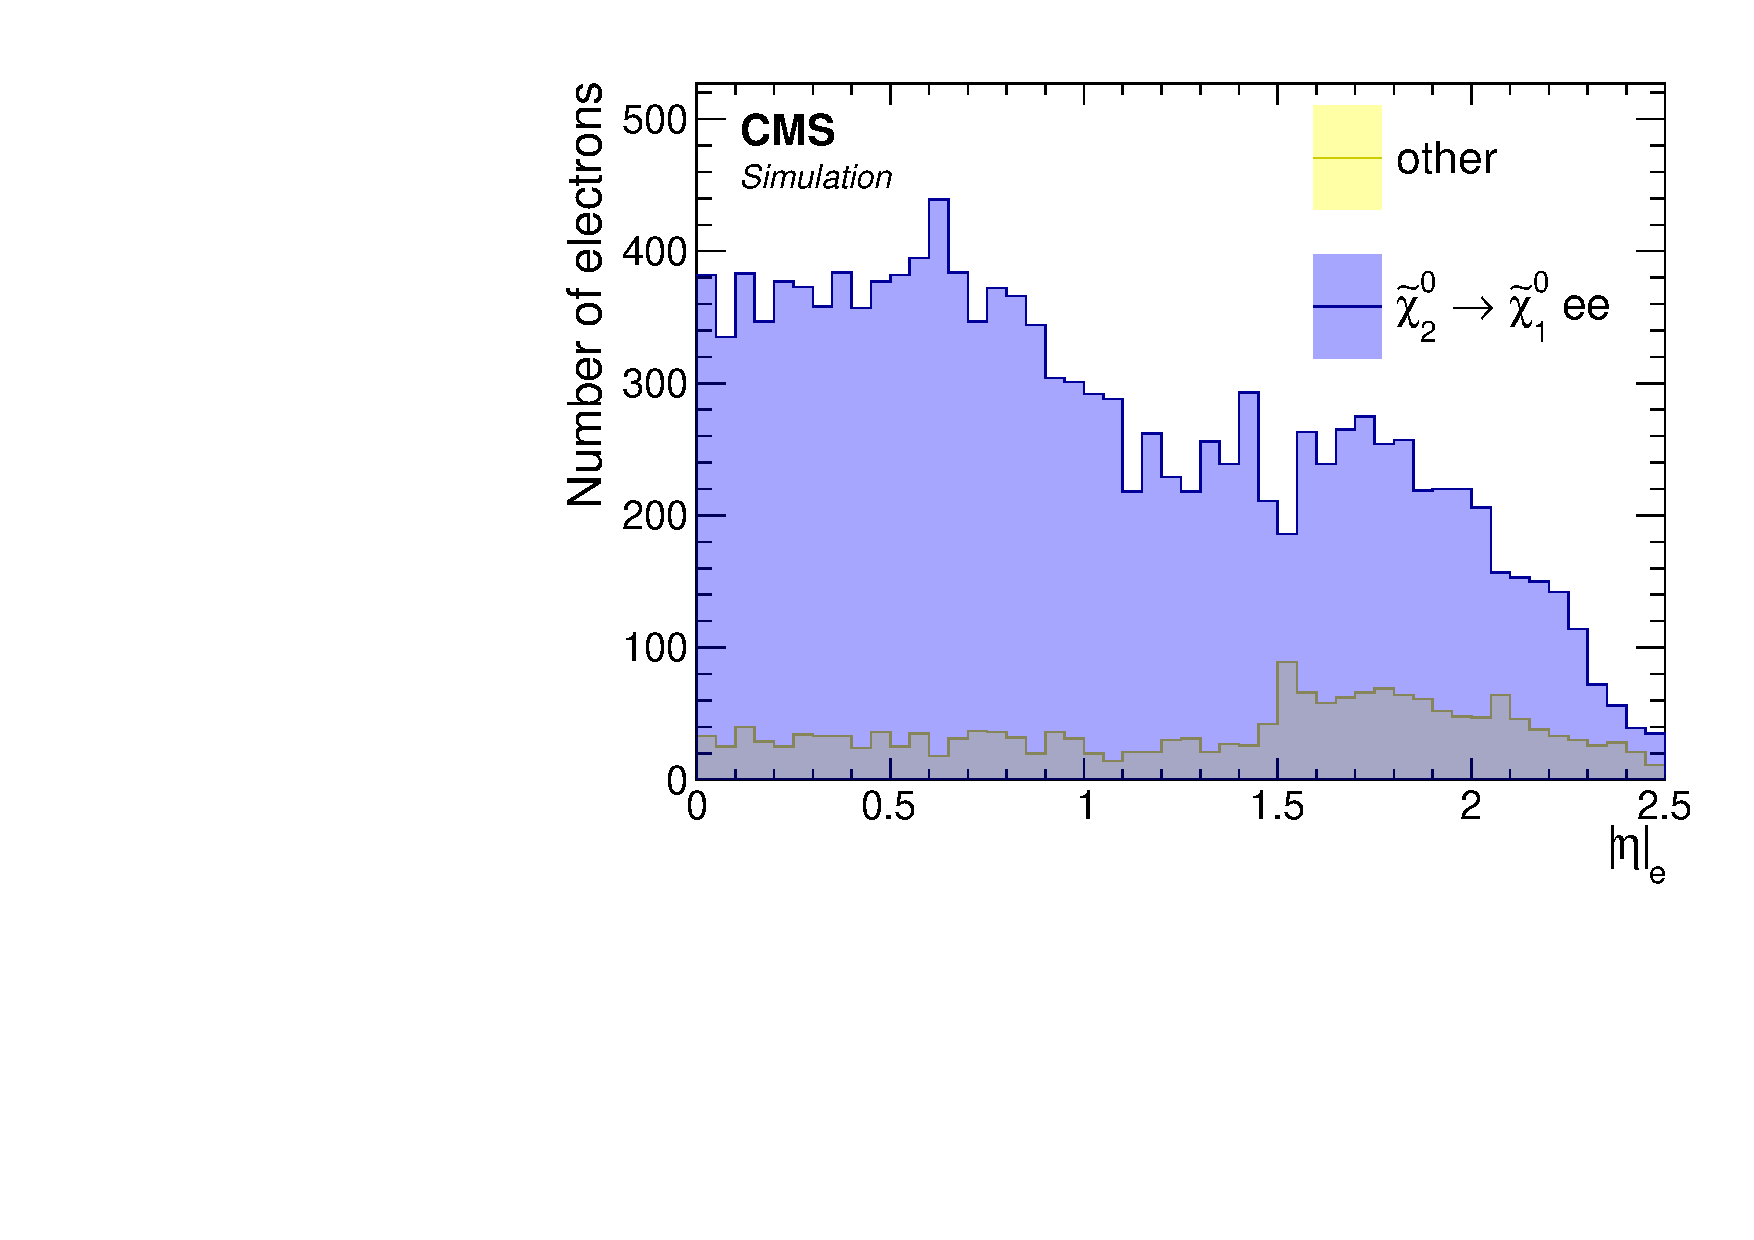
\includegraphics[width=0.48\linewidth]{plots/lepton_selection/lepton_selection_dm5p63/none_Electrons_eta.pdf} \,
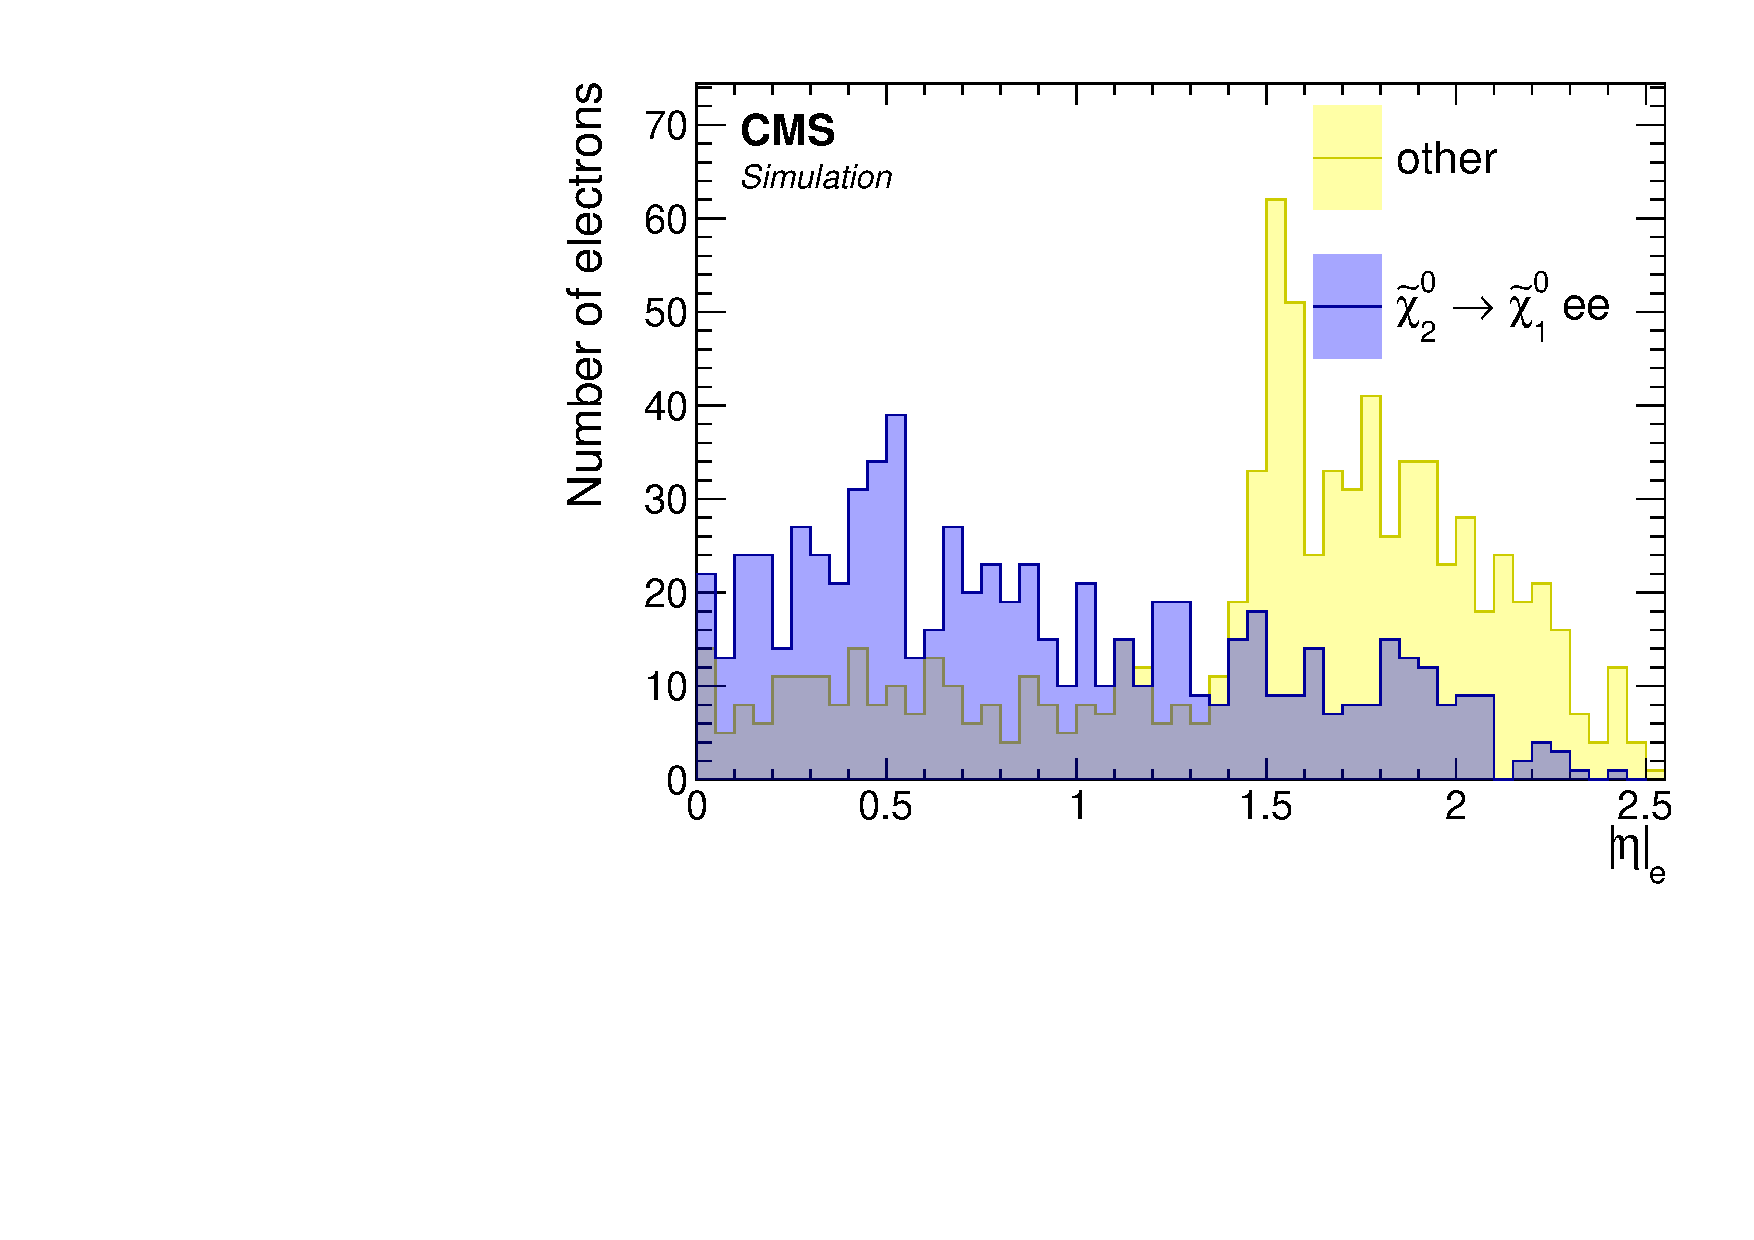
\includegraphics[width=0.48\linewidth]{plots/lepton_selection/lepton_selection_dm1p92/none_Electrons_eta.pdf}  \\
\caption[Distributions of $\abs{\eta}$ of reconstructed electrons with loose ID]{ Distributions of $\abs{\eta}$ of reconstructed electrons with loose ID for $\dm=5.63\GeV$ (left) and $\dm=1.92\GeV$ (right). Cuts of $\DR(\jmath_1,\Pe)>0.4$ and $\pt<15\GeV$ are applied.}
\label{fig:electrons-selection-eta}
\end{figure}

To determine whether a tighter \gls{wp} for the electron-identification is beneficial, the effects of requiring either a Medium or a Tight \gls{wp} are investigated. The \gls{wp} previously used in the distributions is the loose \gls{wp}. Two bins in Figure~\ref{fig:electrons-selection-id} labeled \emph{fail} and \emph{pass} indicate the frequency with which the electron fails or passes the identification criteria of Medium or Tight \glspl{wp}. A considerable fraction of non-signal electrons are rejected in the low \dm case by picking either a Medium or Tight \gls{wp}, but a significant number of signal electrons is also lost. Therefore, using these selections is not very efficient and results in low signal acceptance. The decision is made to use a loose \gls{wp} for the electrons, and instead rely on isolation to achieve higher purity.

The effect of isolation on the purity of the electrons is also examined. A custom jet-based isolation is discussed in detail in Section~\ref{sec:isolation}, but for the sake of completeness, its effect on the purity of the electrons is also shown here. The custom jet-based isolation is compared with the standard definition of lepton isolation. Note that the later does not take into account the possibility that two electrons can be produced with a small angle of separation (small \DR), as is the case for signal models with small \dm. The isolation distributions are shown in Figure~\ref{fig:electrons-selection-isolation}.

\begin{figure}[!htb]
\centering
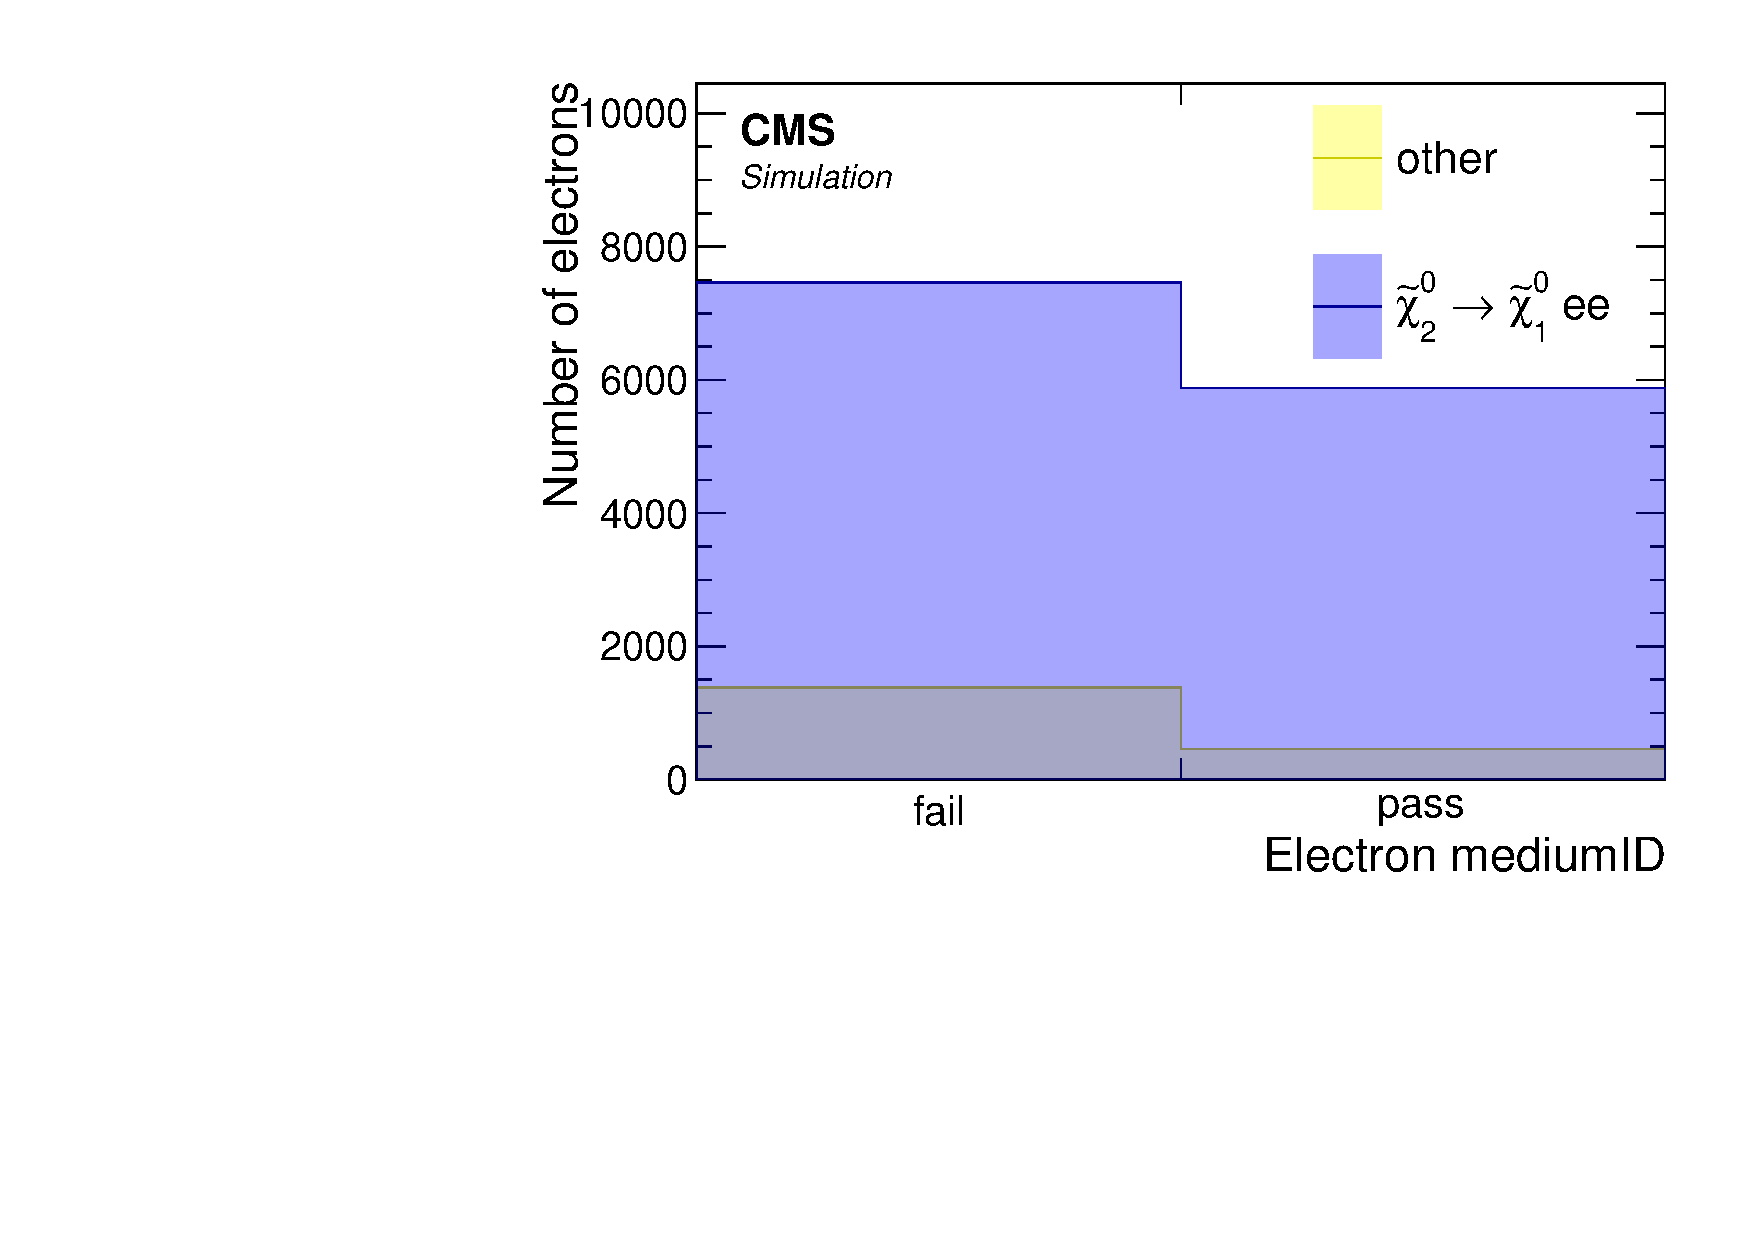
\includegraphics[width=0.48\linewidth]{plots/lepton_selection/lepton_selection_dm5p63/none_Electrons_medium.pdf} \,
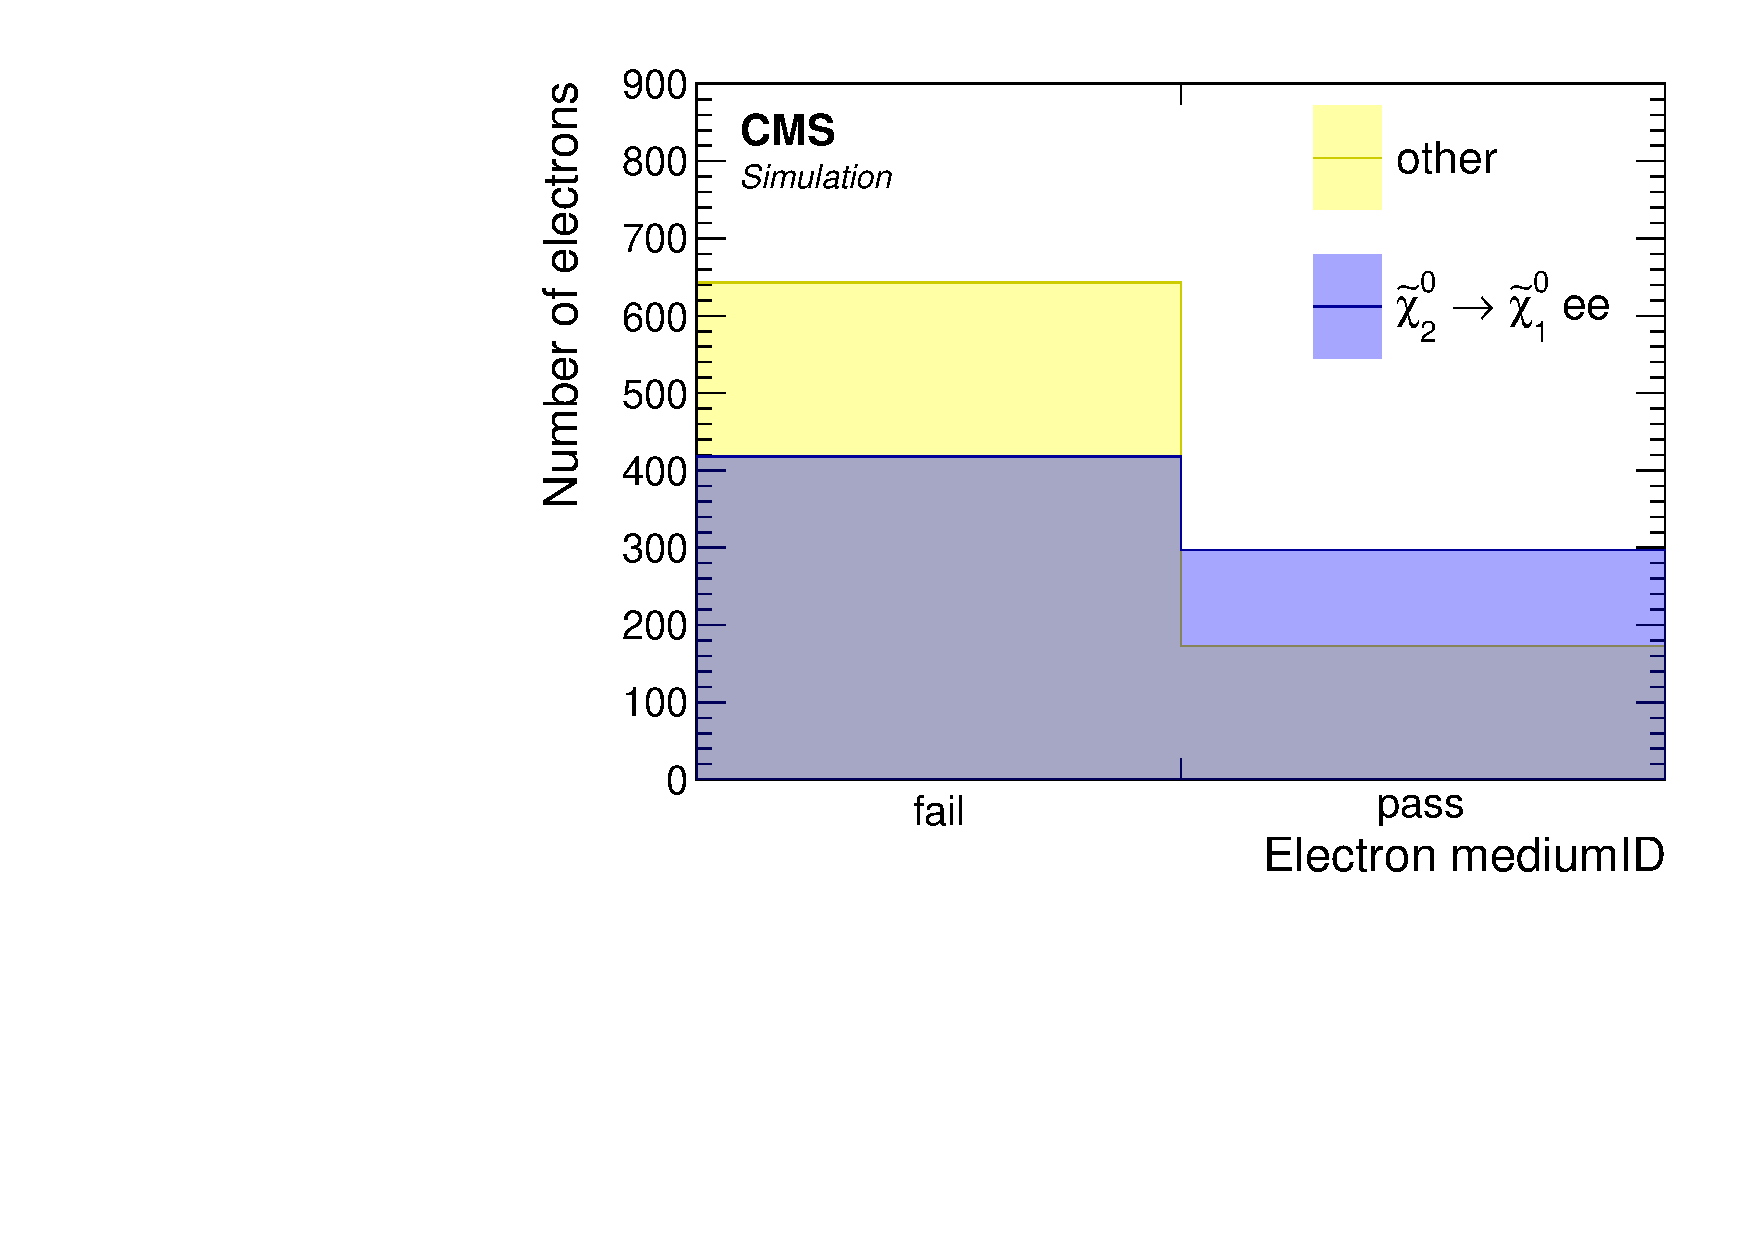
\includegraphics[width=0.48\linewidth]{plots/lepton_selection/lepton_selection_dm1p92/none_Electrons_medium.pdf}  \\
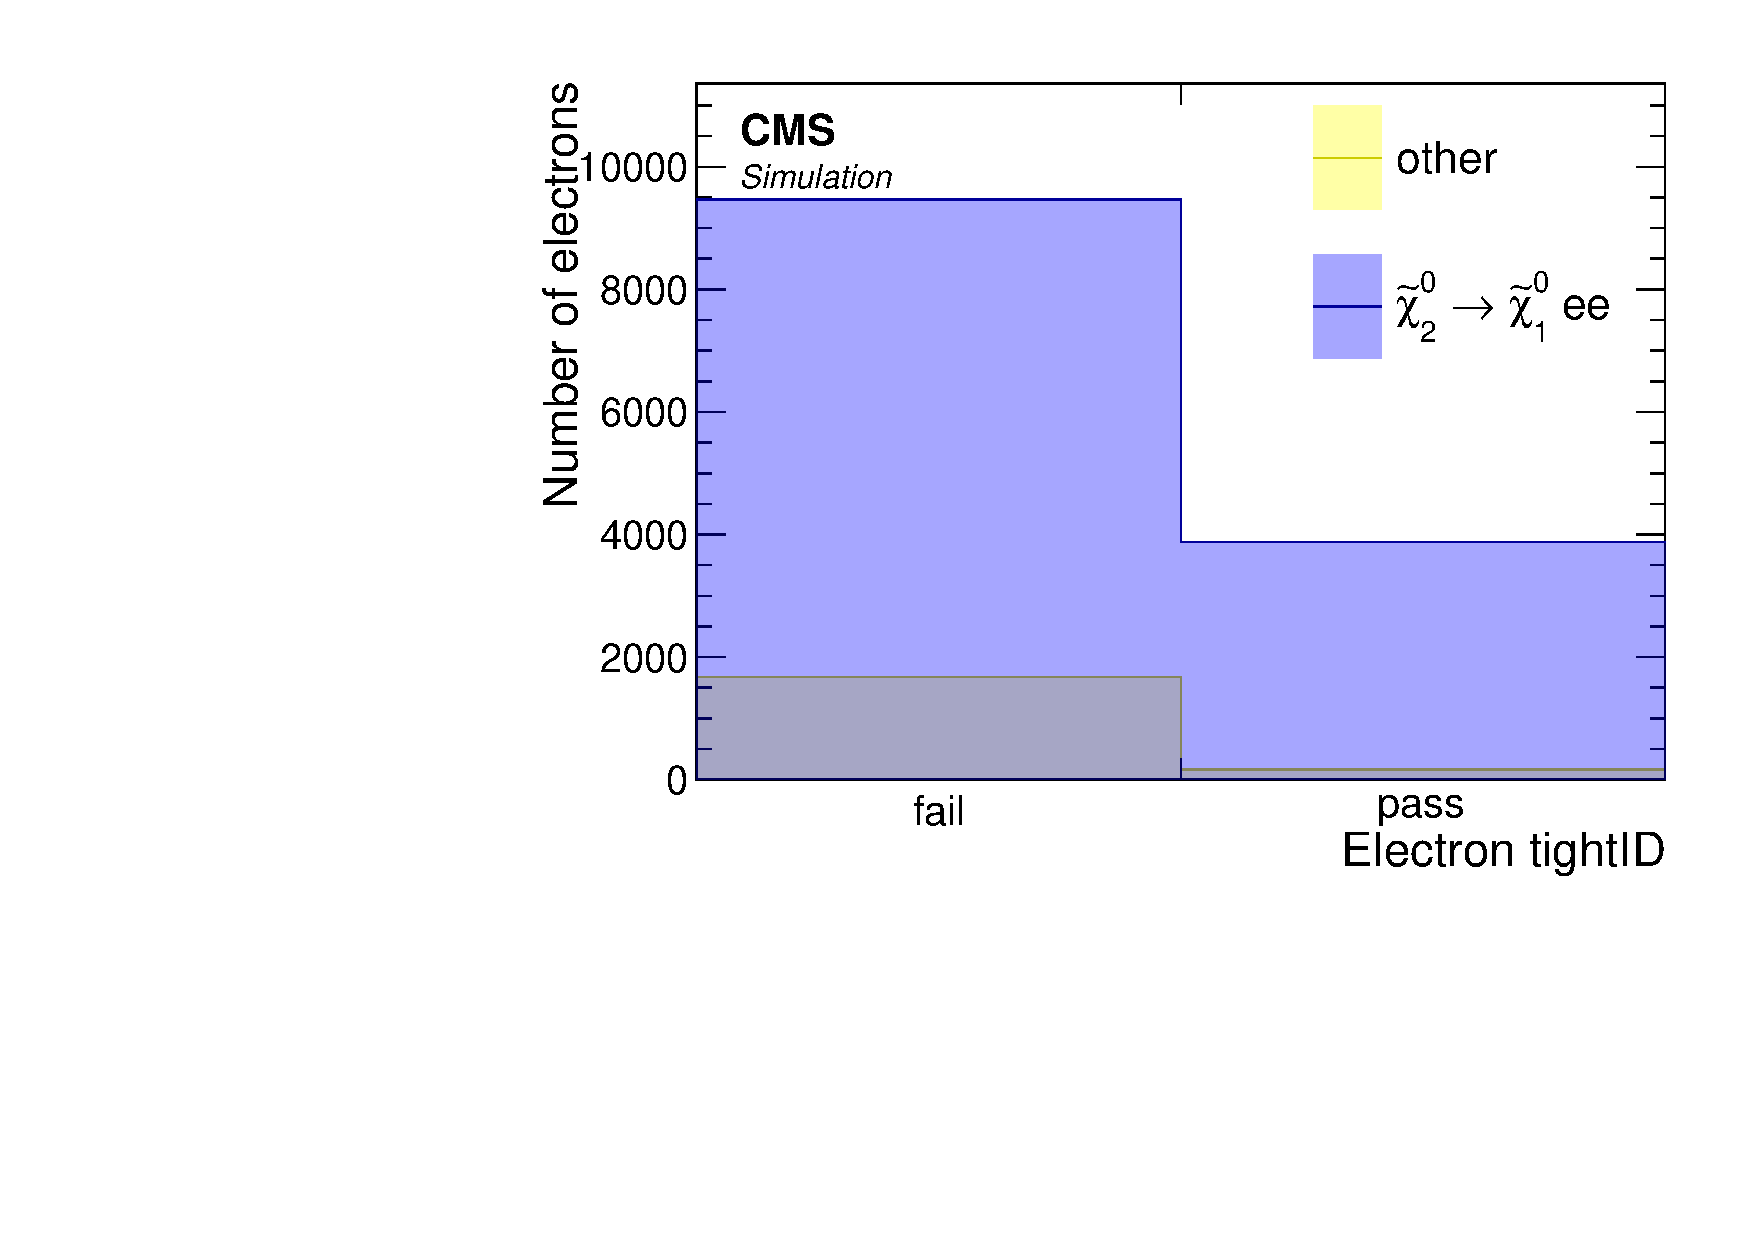
\includegraphics[width=0.48\linewidth]{plots/lepton_selection/lepton_selection_dm5p63/none_Electrons_tight.pdf} \,
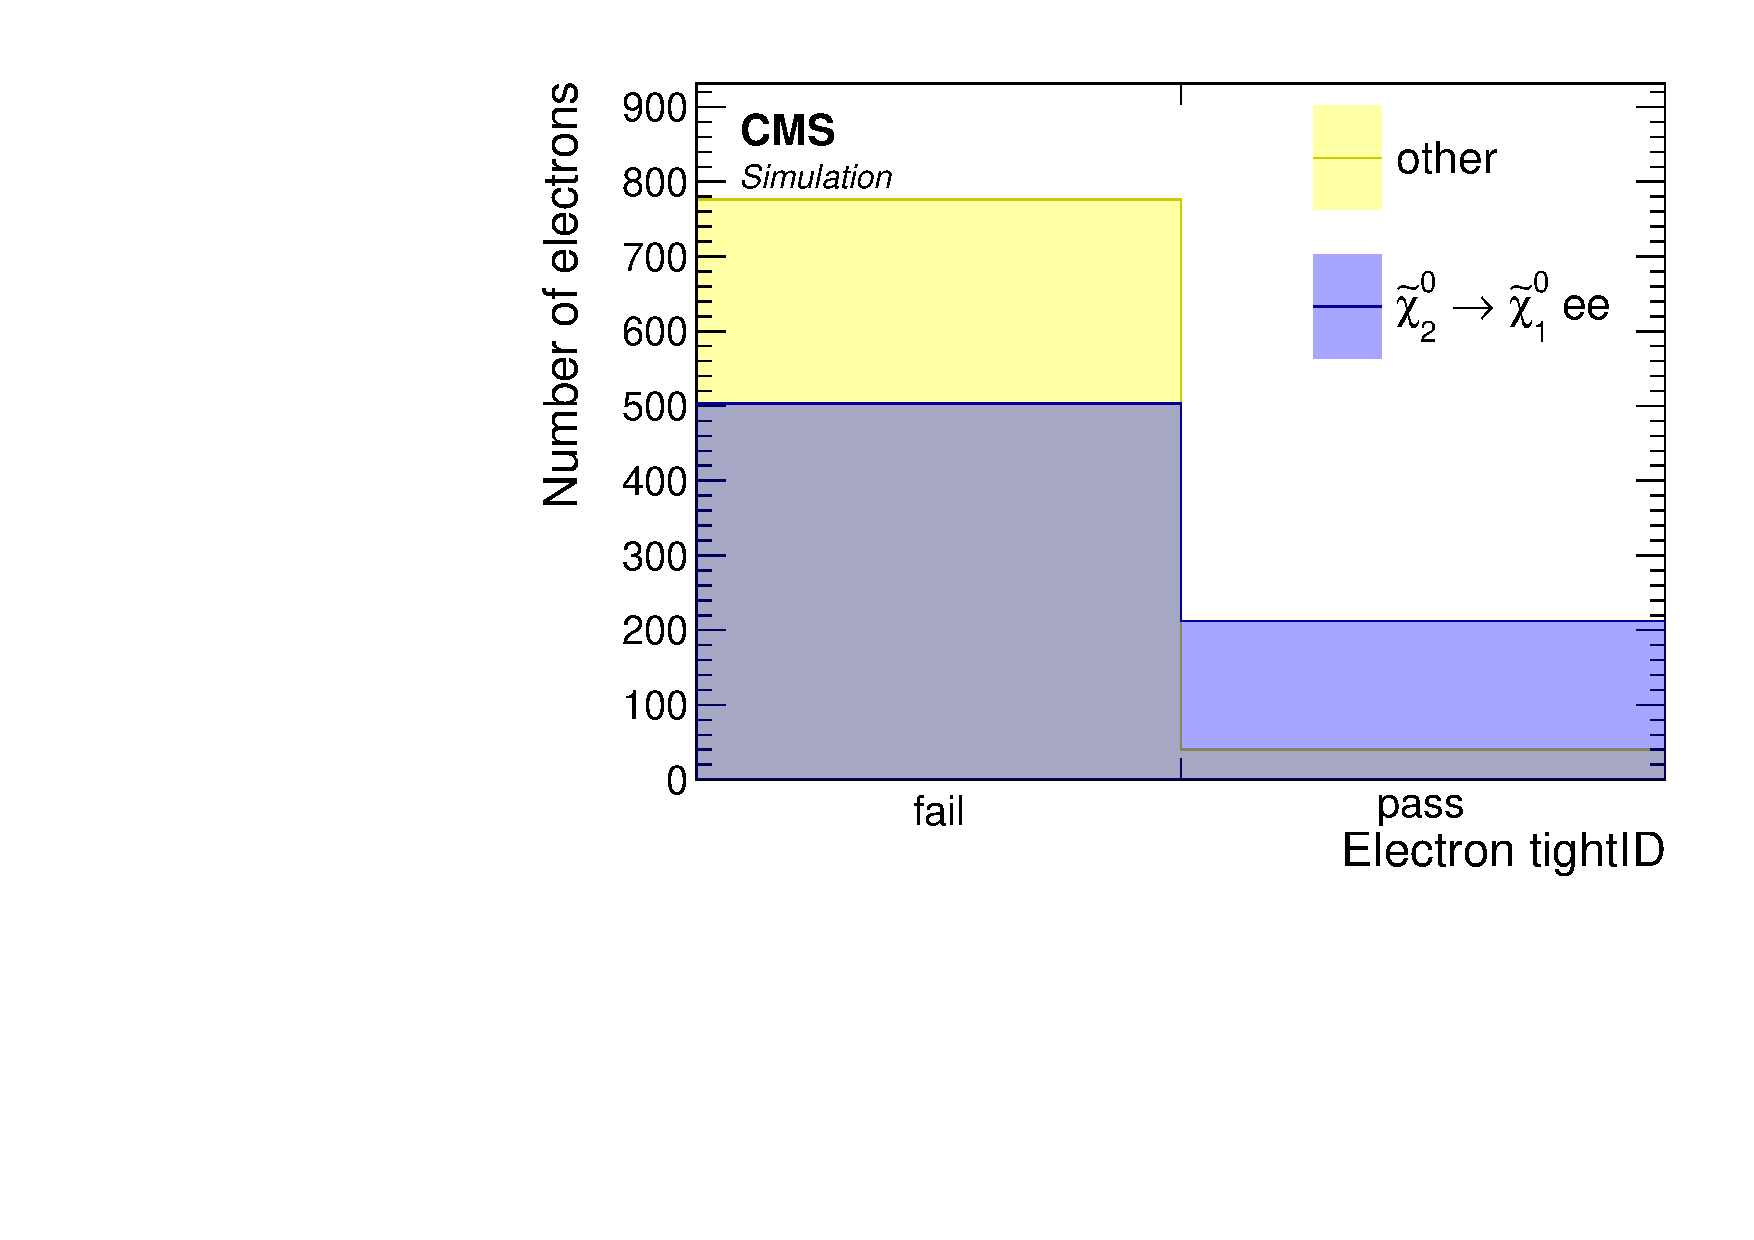
\includegraphics[width=0.48\linewidth]{plots/lepton_selection/lepton_selection_dm1p92/none_Electrons_tight.pdf}  \\
\caption[Medium and Tight ID \glspl{wp} distribution of reconstructed electrons]{Medium (top) and Tight (bottom) ID \glspl{wp} distributions of reconstructed electrons for $\dm=5.63\GeV$ (left) and $\dm=1.92\GeV$ (right). Cuts of $\DR(\jmath_1,\Pe)>0.4$ and $\pt<15\GeV$ are applied to the electrons.}
\label{fig:electrons-selection-id}
\end{figure}

\begin{figure}[!htb]
\centering
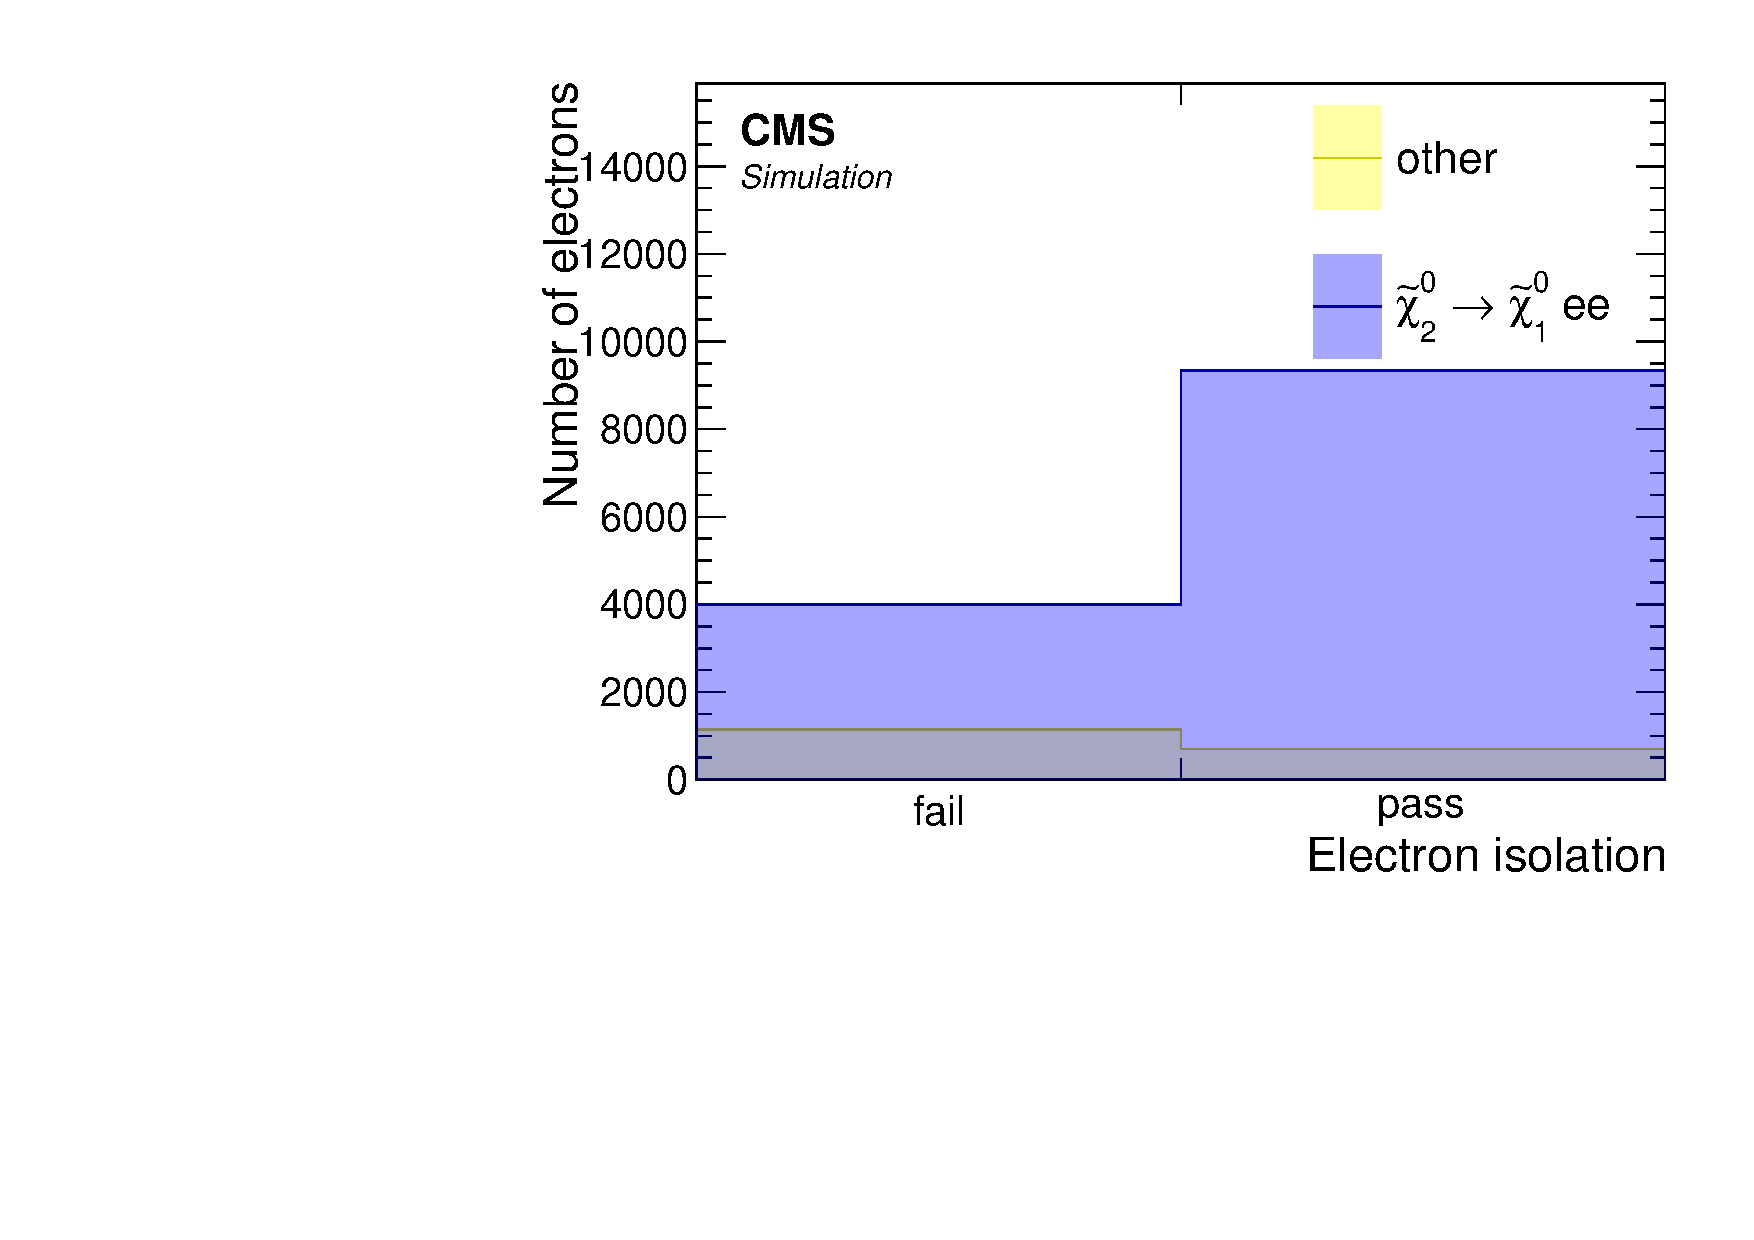
\includegraphics[width=0.48\linewidth]{plots/lepton_selection/lepton_selection_dm5p63/none_Electrons_iso.pdf} \,
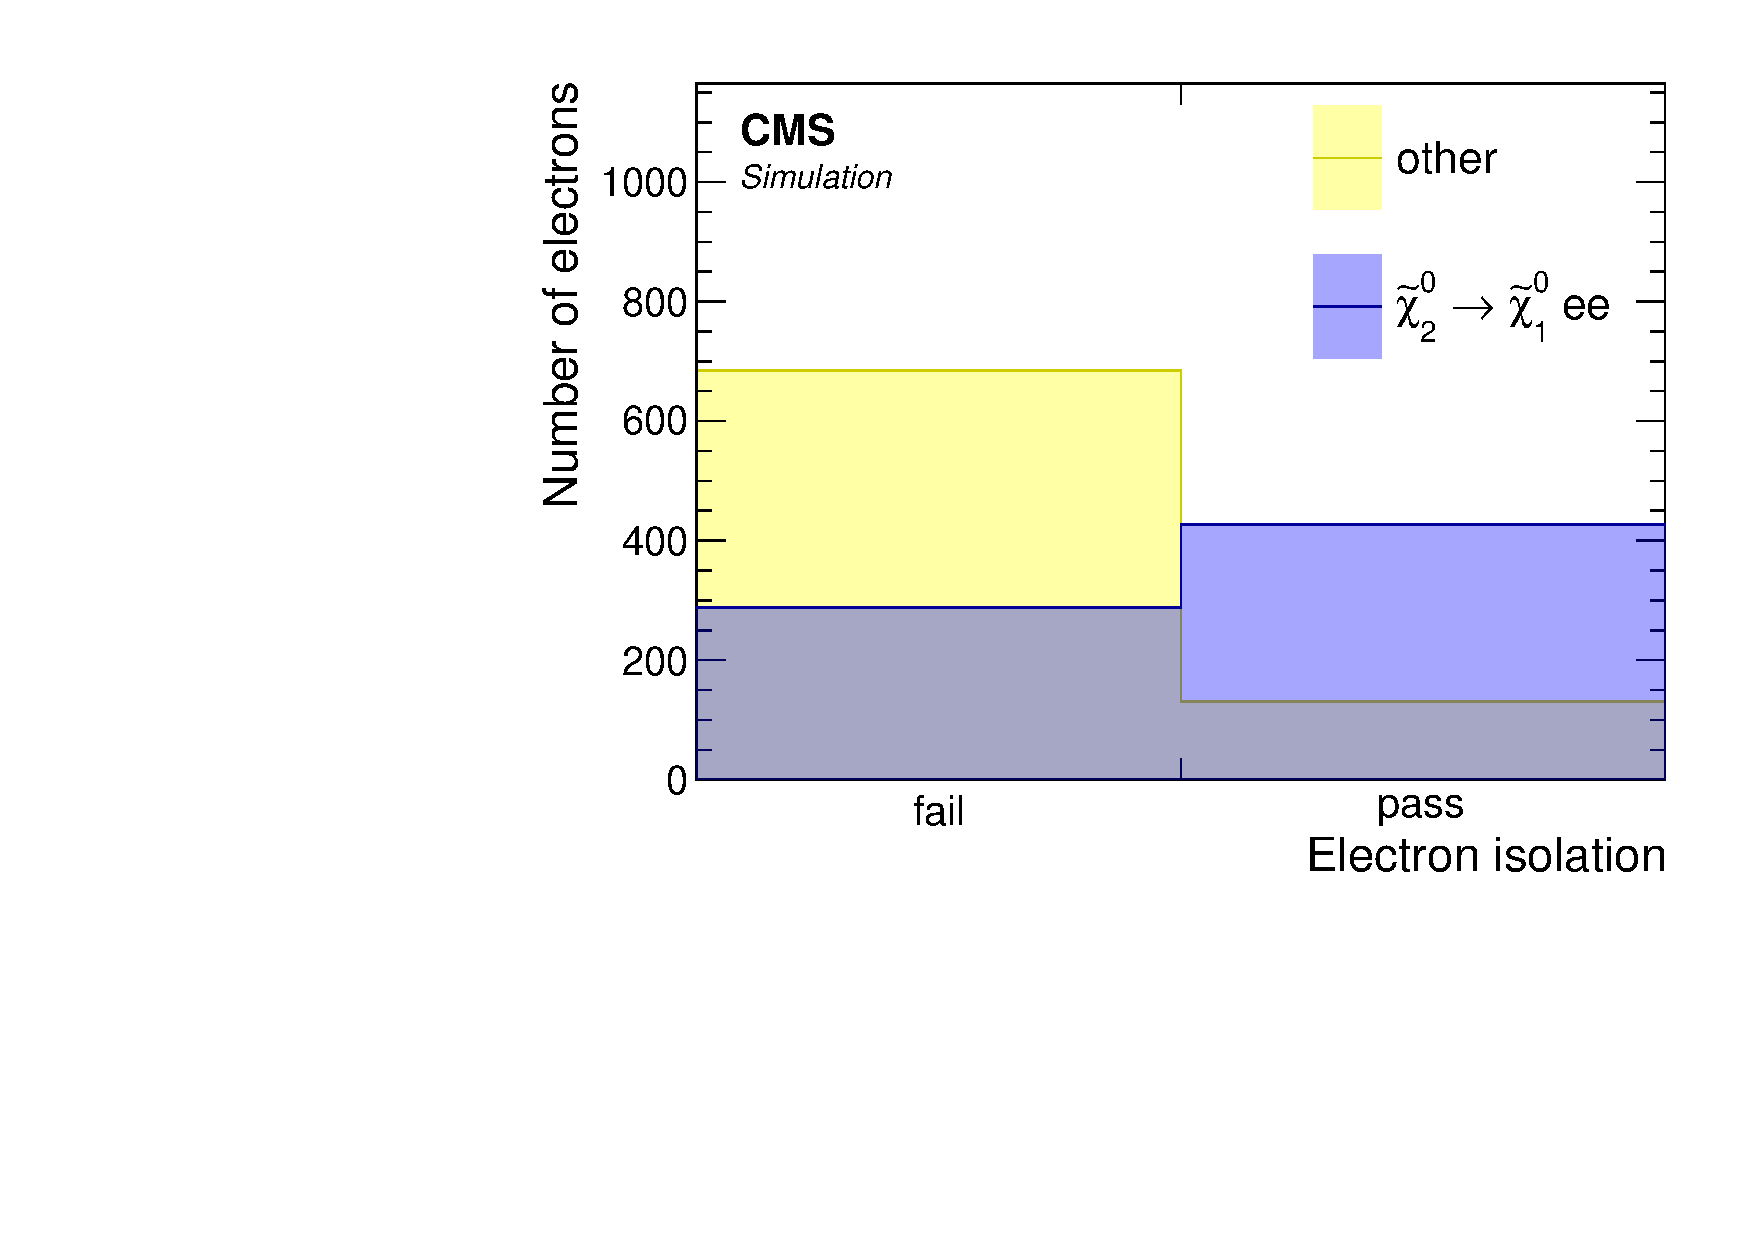
\includegraphics[width=0.48\linewidth]{plots/lepton_selection/lepton_selection_dm1p92/none_Electrons_iso.pdf}  \\
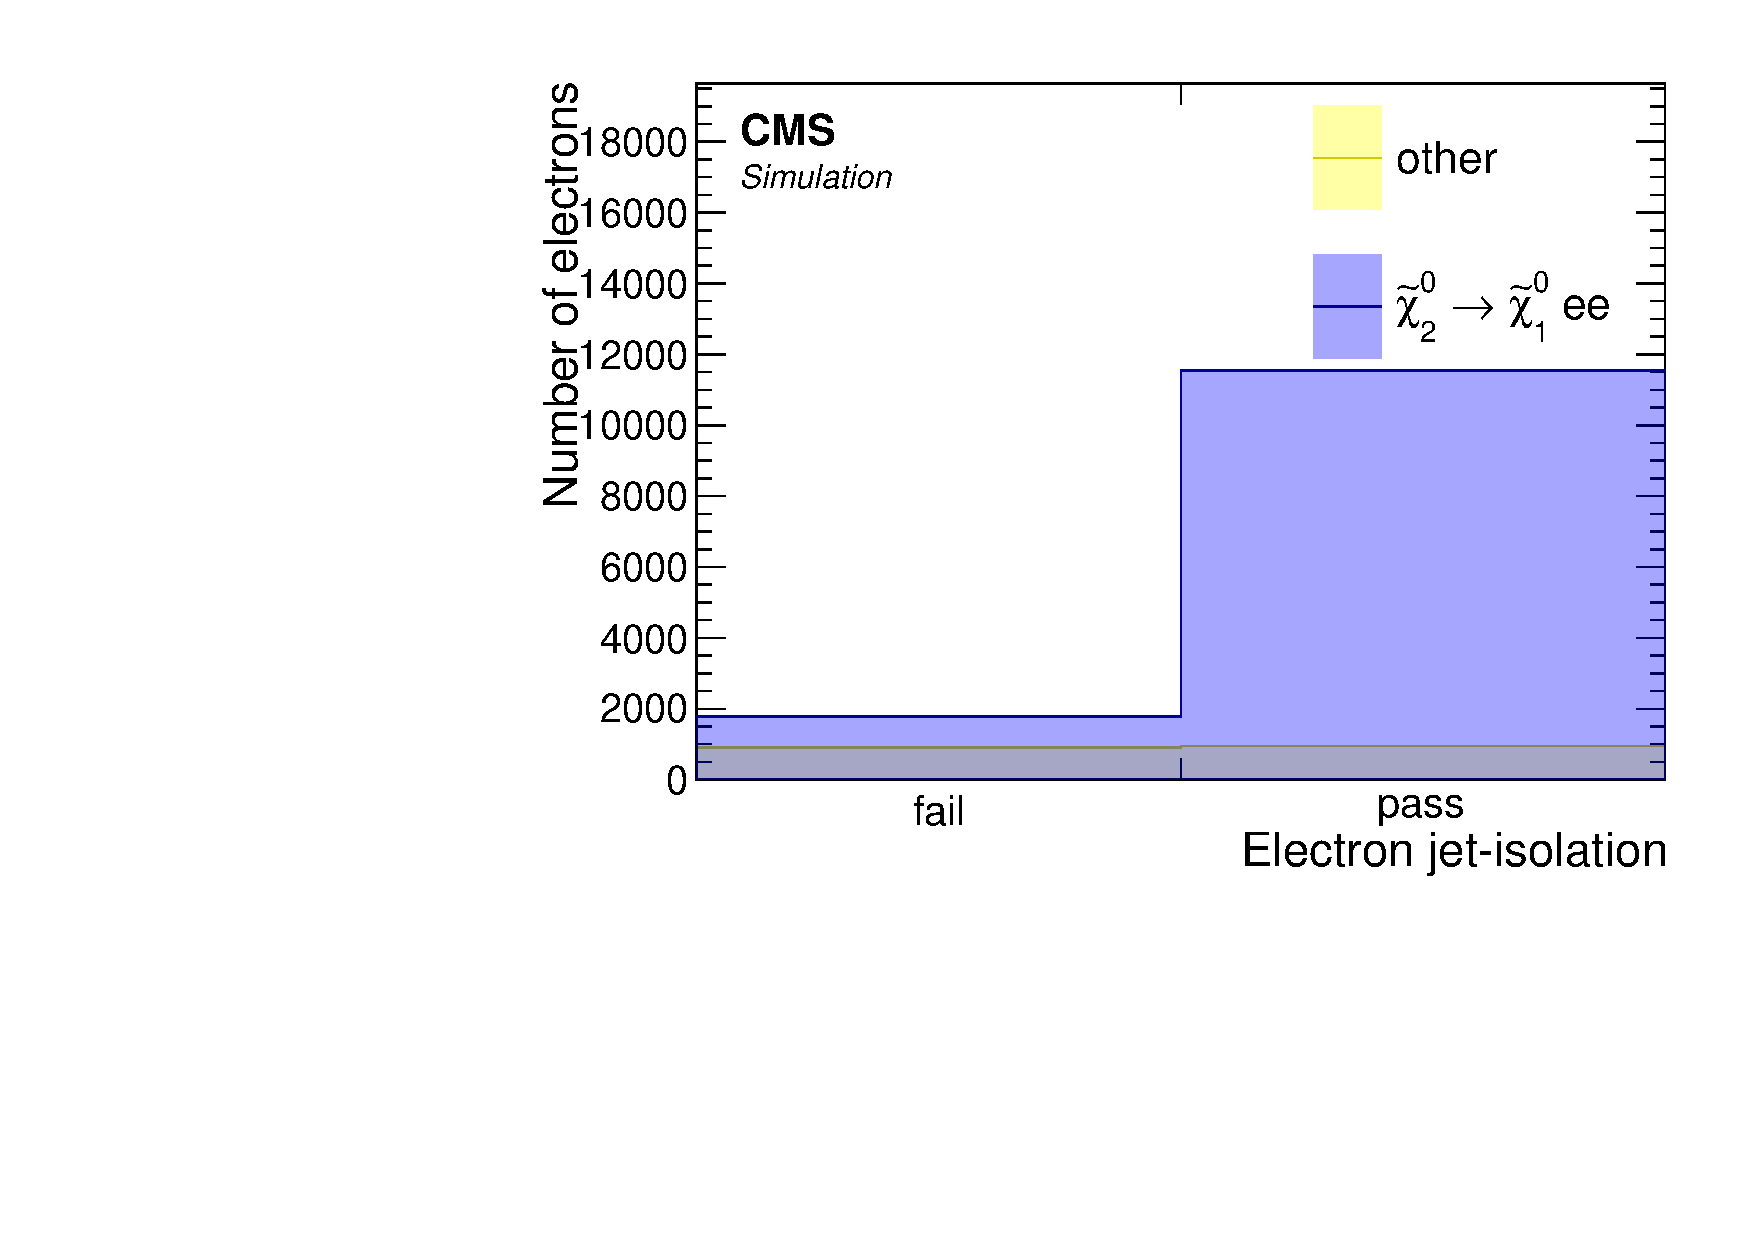
\includegraphics[width=0.48\linewidth]{plots/lepton_selection/lepton_selection_dm5p63/none_Electrons_CorrJetNoMultIso11Dr0.5.pdf} \,
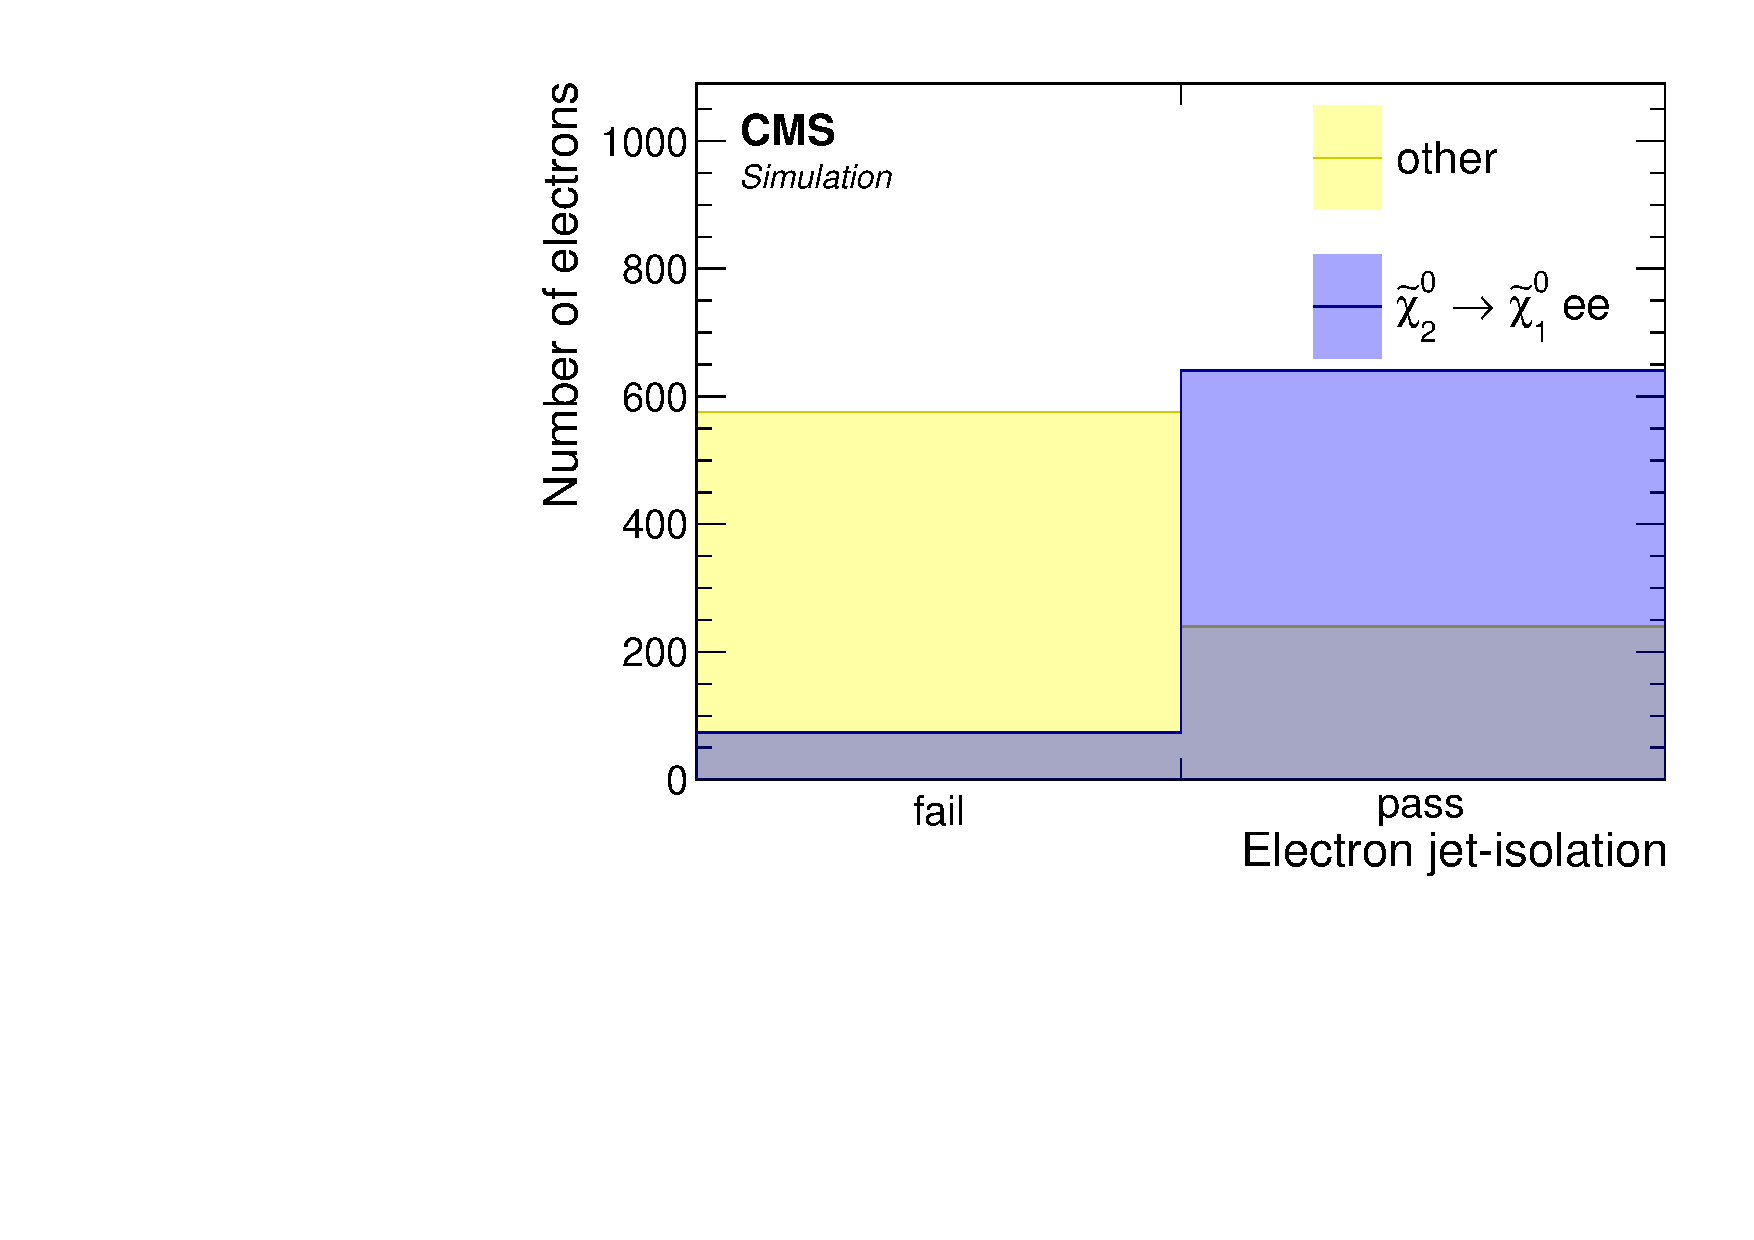
\includegraphics[width=0.48\linewidth]{plots/lepton_selection/lepton_selection_dm1p92/none_Electrons_CorrJetNoMultIso11Dr0.5.pdf}  \\
\caption[standard isolation and jet-isolation distribution of reconstructed electrons]{Standard isolation (top) and custom jet-isolation (bottom) distributions of reconstructed electrons with loose ID for $\dm=5.63\GeV$ (left) and $\dm=1.92\GeV$ (right). Cuts of $\DR(\jmath_1,\Pe)>0.4$ and $\pt<15\GeV$ are applied.}
\label{fig:electrons-selection-isolation}
\end{figure}

The standard lepton isolation is not efficient for both \dm cases, while the custom jet-isolation performs well in terms of signal electron efficiency and successfully rejects a considerable amount of non-signal electrons. This results in a purer sample of electrons, and thus the choice of custom jet-isolation is concluded to be favorable. The effect of this choice on the $\eta$ distribution is also examined in Figure~\ref{fig:electrons-selection-eta-jet-iso}, concluding the selection of electrons. The custom jet-isolation optimally purifies the electron sample while retaining a high signal efficiency, compared to distributions in Figure~\ref{fig:electrons-selection-eta}.

\begin{figure}[!htb]
\centering
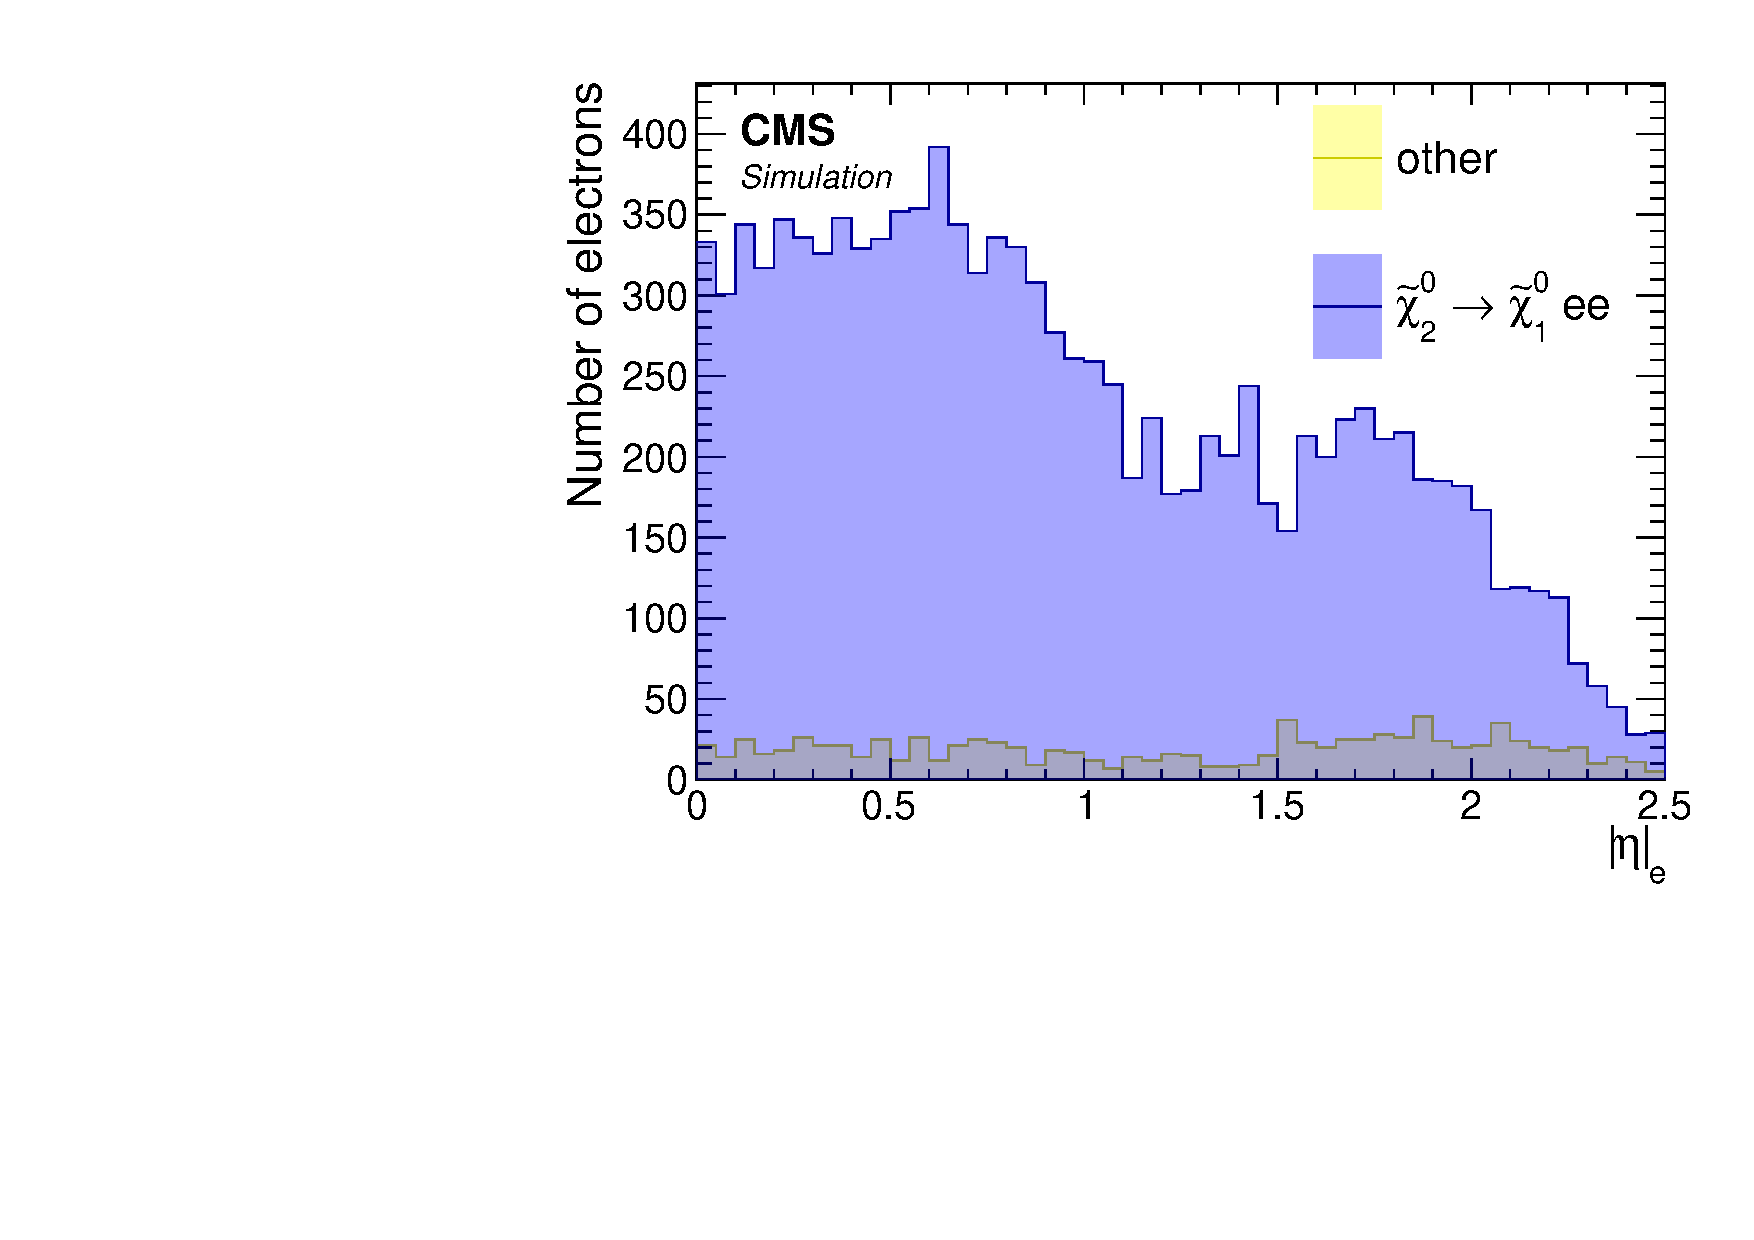
\includegraphics[width=0.48\linewidth]{plots/lepton_selection/lepton_selection_dm5p63/none_Electrons_eta_jet_iso.pdf} \,
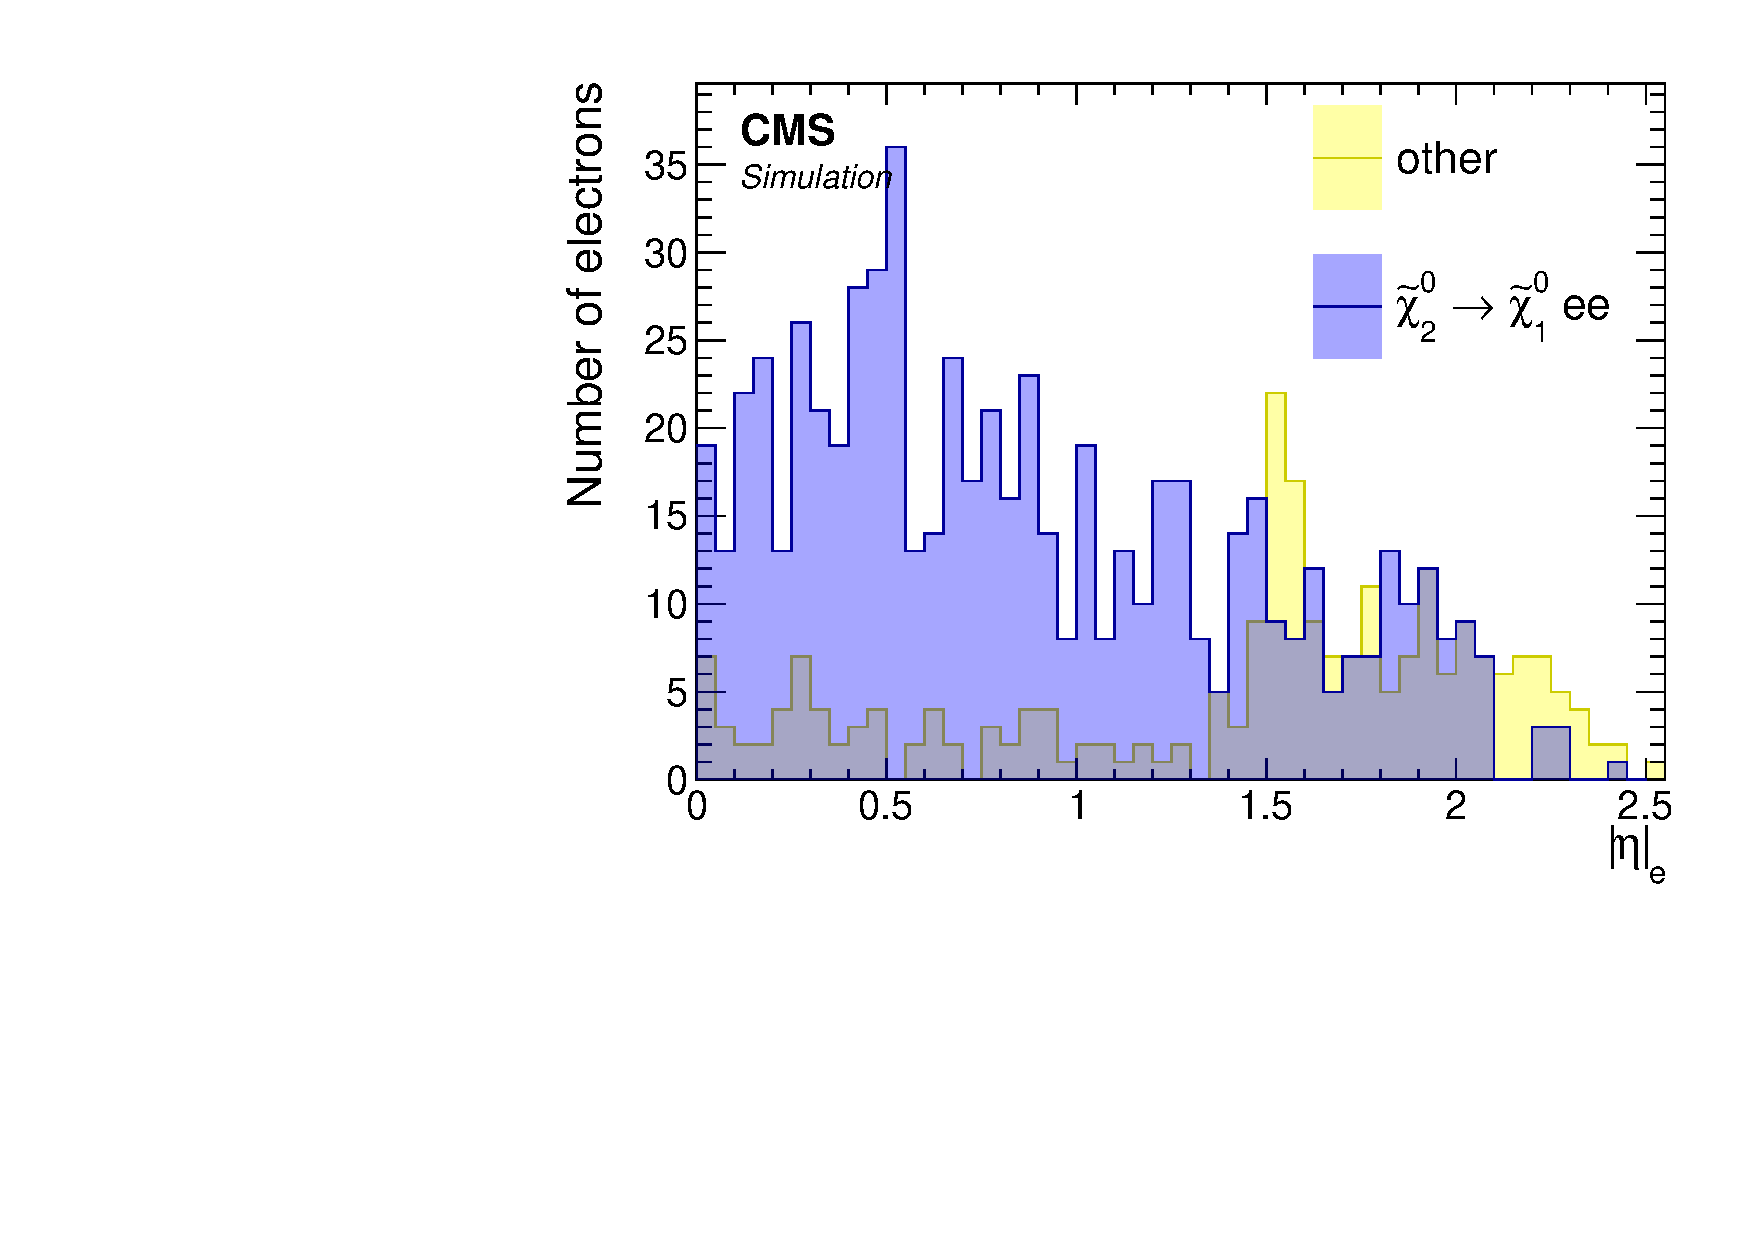
\includegraphics[width=0.48\linewidth]{plots/lepton_selection/lepton_selection_dm1p92/none_Electrons_eta_jet_iso.pdf}  \\
\caption[$\abs{\eta}$ distribution of reconstructed electrons with loose ID passing jet-isolation]{ $\abs{\eta}$ distribution of reconstructed electrons with loose ID passing jet-isolation for $\dm=5.63\GeV$ (left) and $\dm=1.92\GeV$ (right). Cuts of $\DR(\jmath_1,\Pe)>0.4$ and $\pt<15\GeV$ are applied.}
\label{fig:electrons-selection-eta-jet-iso}
\end{figure}

In summary, the following is the full set of selection criteria the analysis electrons:

\begin{itemize}
\item $5<\pt<15\GeV$;
\item $\abs{\eta} < 2.5$;
\item $\DR(\jmath_1,\Pe)>0.4$;
\item loose ID \gls{wp};
\item pass jet-isolation.
\end{itemize}

\clearpage

\subsection{Muons}
\label{sec:muon-selection}

The \pt threshold for reconstructed muons is significantly lower than that of electrons, making this channel particularly promising in terms of signal acceptance for low \dm models. As was the case for electrons, the initial \gls{wp} choice for reconstructed muons is loose (more information in~\ref{sec:reconstruction-and-identification}), and an analogous procedure is now followed for muons. The angular separation of muons from the leading jet in the event, $\DR(\jmath_1,\mu)$, is the first distribution examined. As shown in Figure~\ref{fig:signal-pt-barrel-endcaps}, the muon endcaps are capable of reconstructing muons with $\pt<3\GeV$ while the barrel is not. Therefore, a split view of barrel and endcaps is shown in Figure~\ref{fig:muons-dr-lj}. Because the endcaps accept muons with lower \pt than the barrel, and because of the generally higher occupancy of tracks in the forward region, the purity in the endcaps is much lower than that in the barrel. The selection developed here attempts to further purify the somewhat contaminated barrel muon sample. Muons with $\DR(\jmath_1,\mu)>0.4$ are selected as in the electrons case, and this selection will apply for the rest of the section.

\begin{figure}[!htb]
\centering
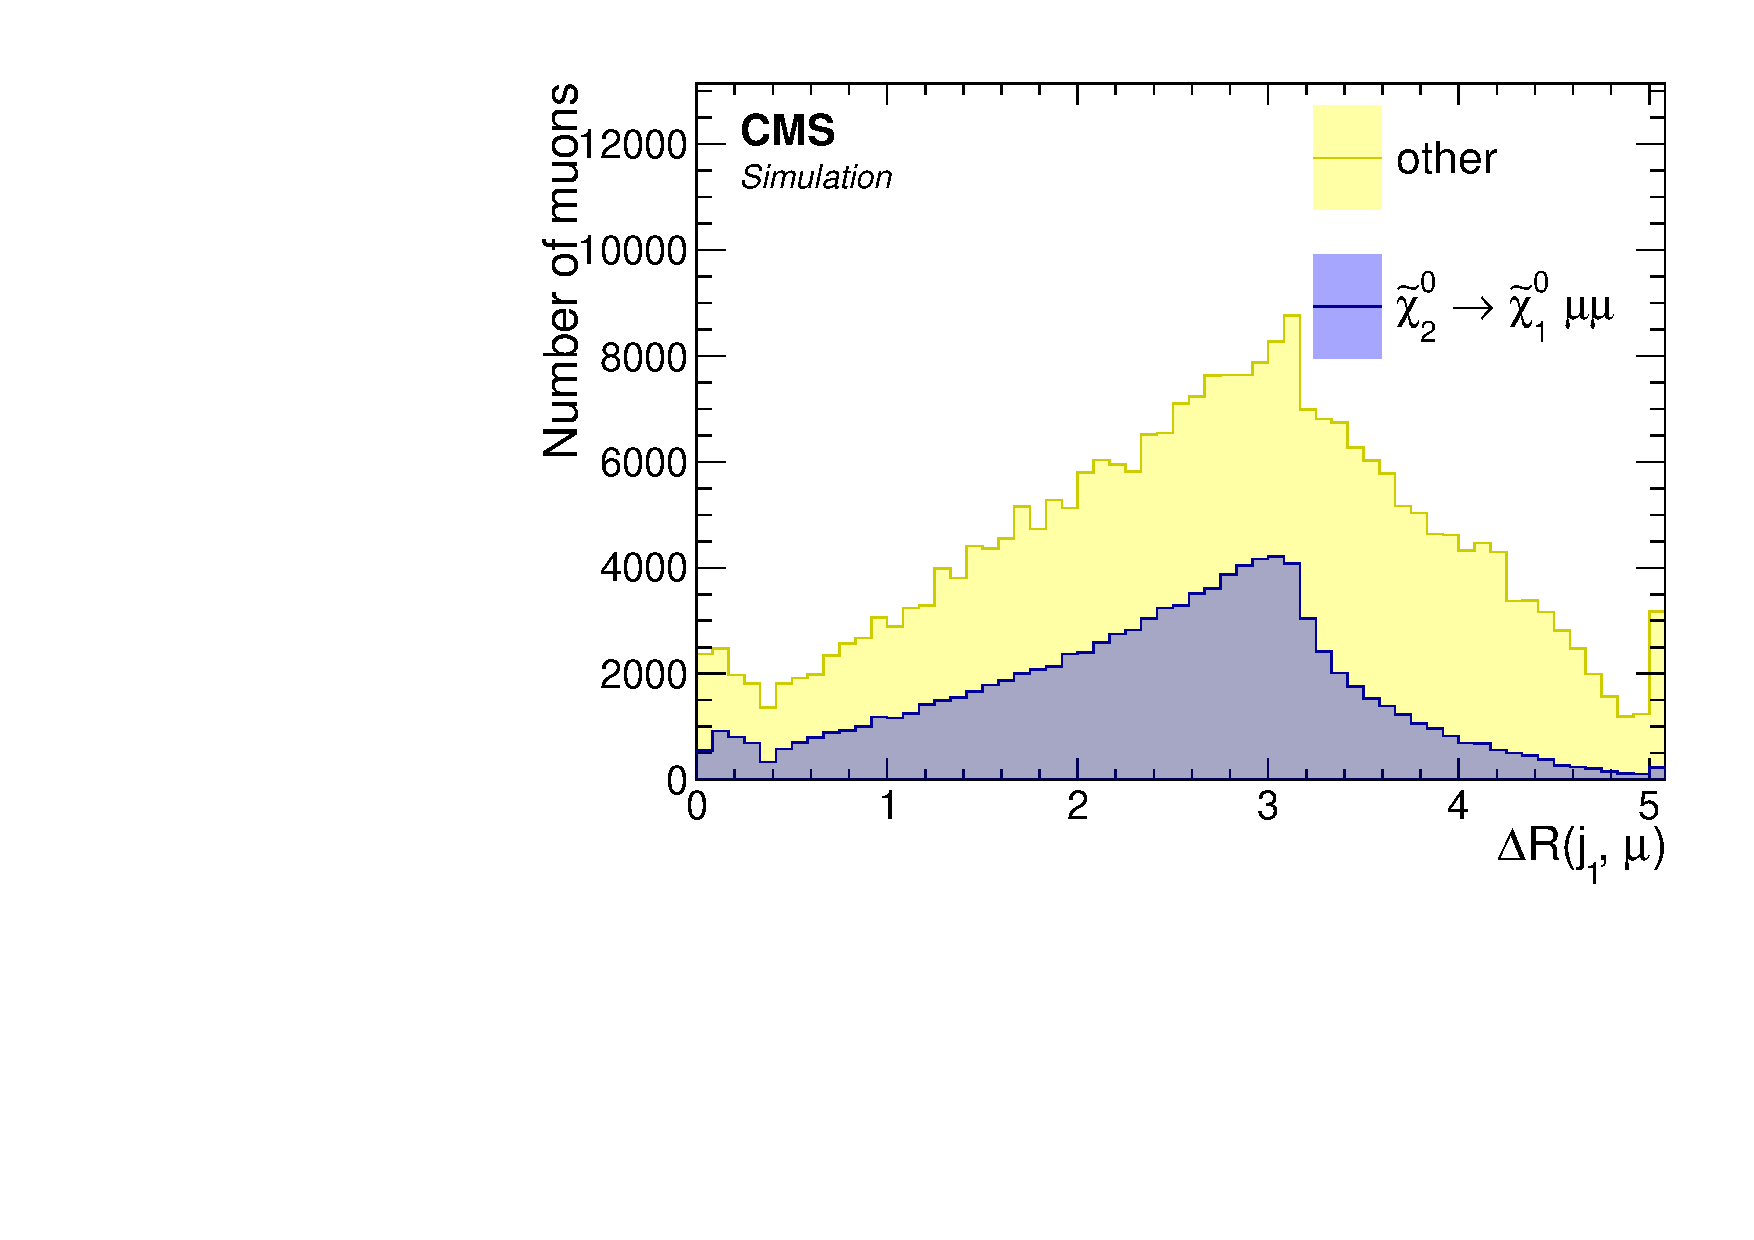
\includegraphics[width=0.32\linewidth]{plots/lepton_selection/lepton_selection_dm5p63/none_Muons_rlj.pdf} \,
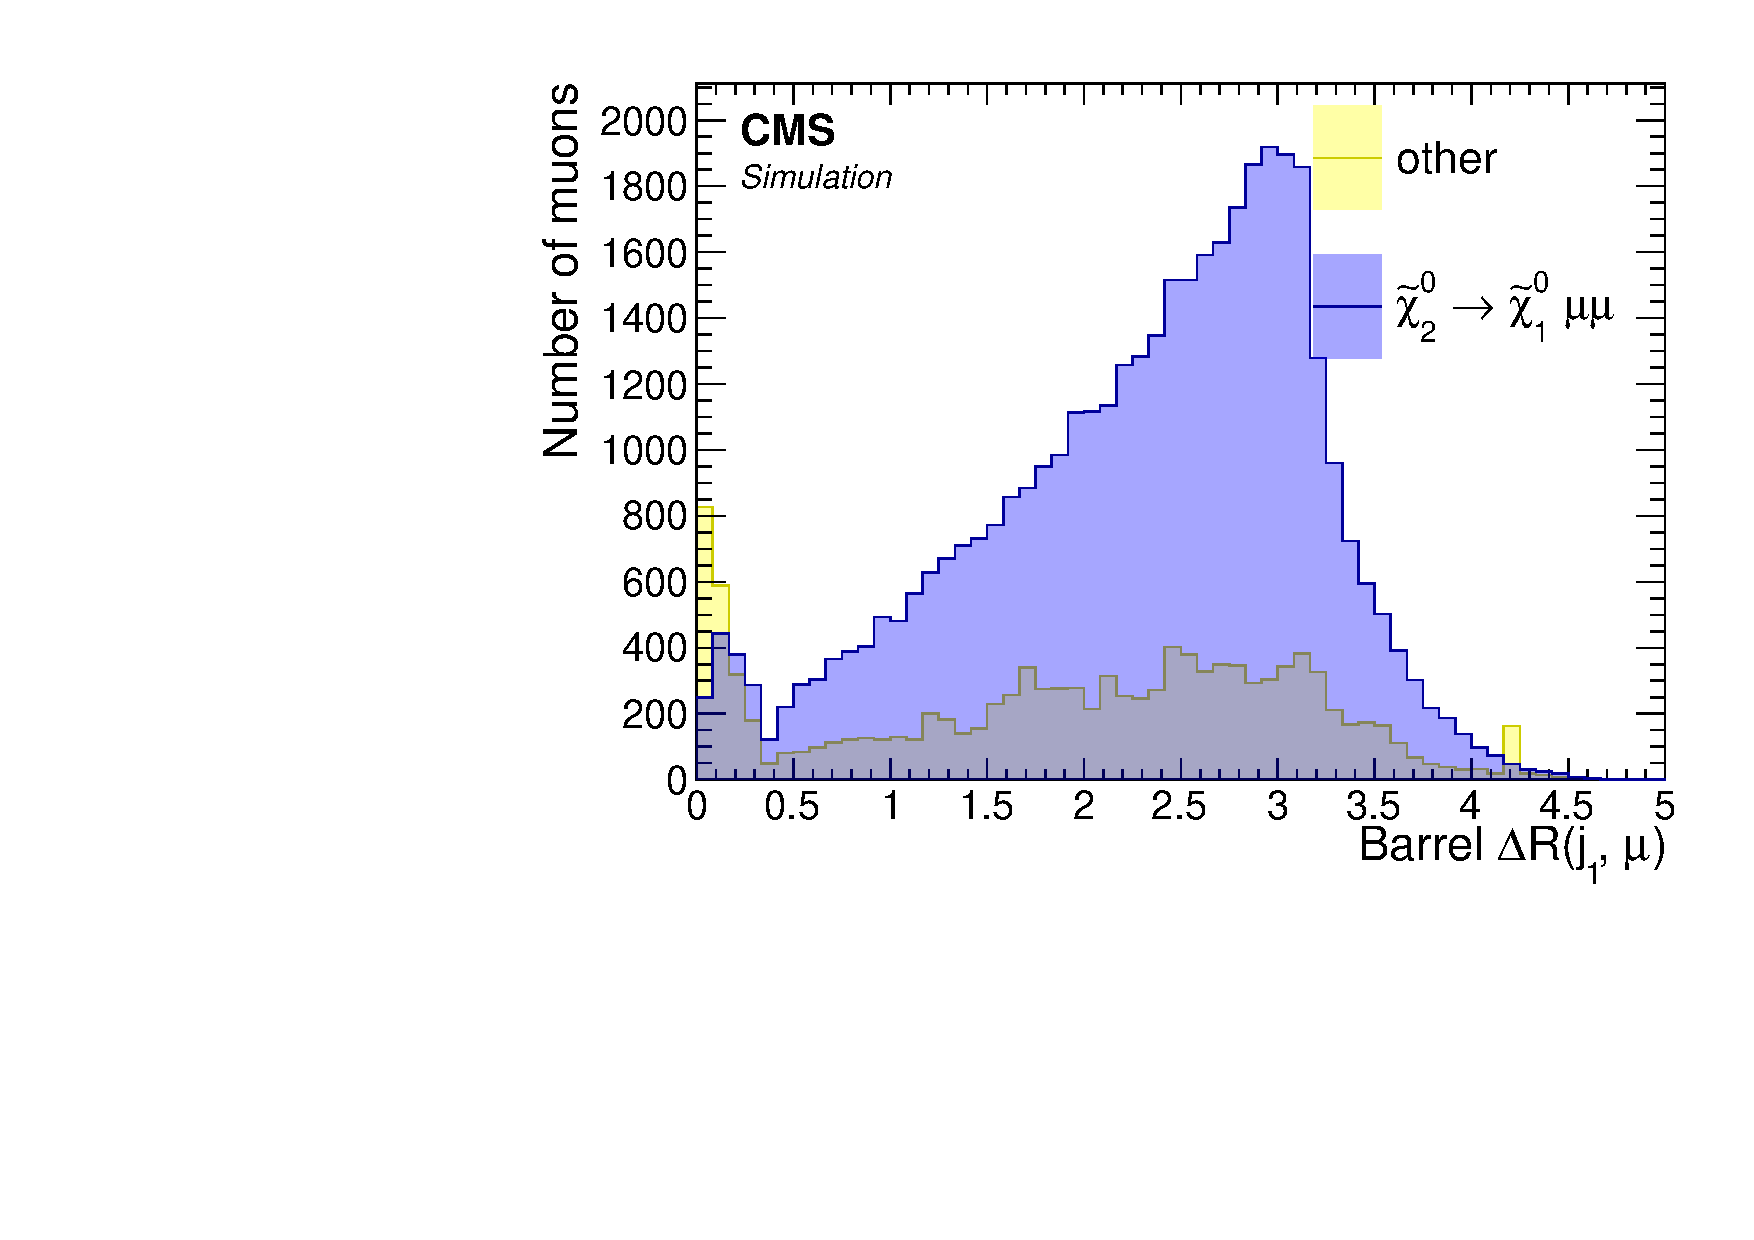
\includegraphics[width=0.32\linewidth]{plots/lepton_selection/lepton_selection_dm5p63/none_Muons_rlj_barrel.pdf}
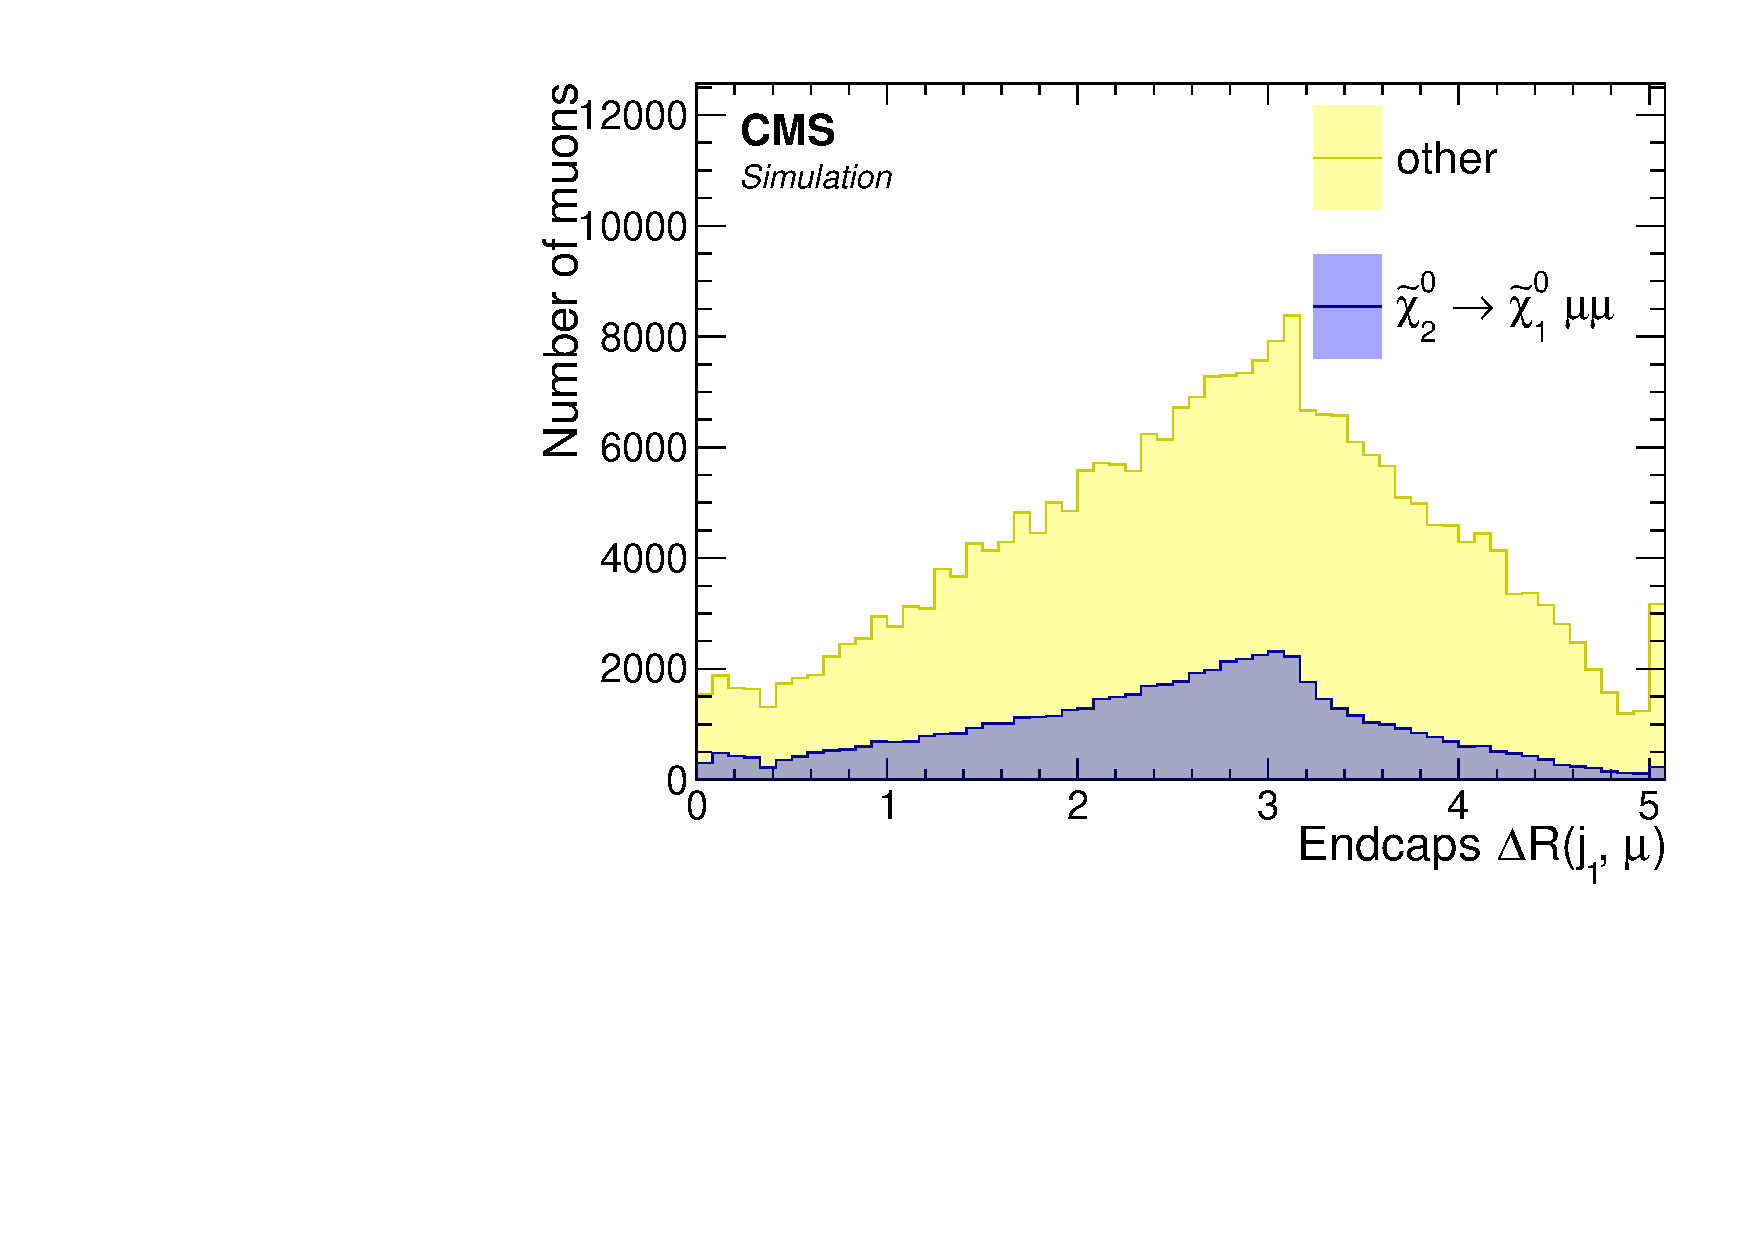
\includegraphics[width=0.32\linewidth]{plots/lepton_selection/lepton_selection_dm5p63/none_Muons_rlj_endcape.pdf}  \\
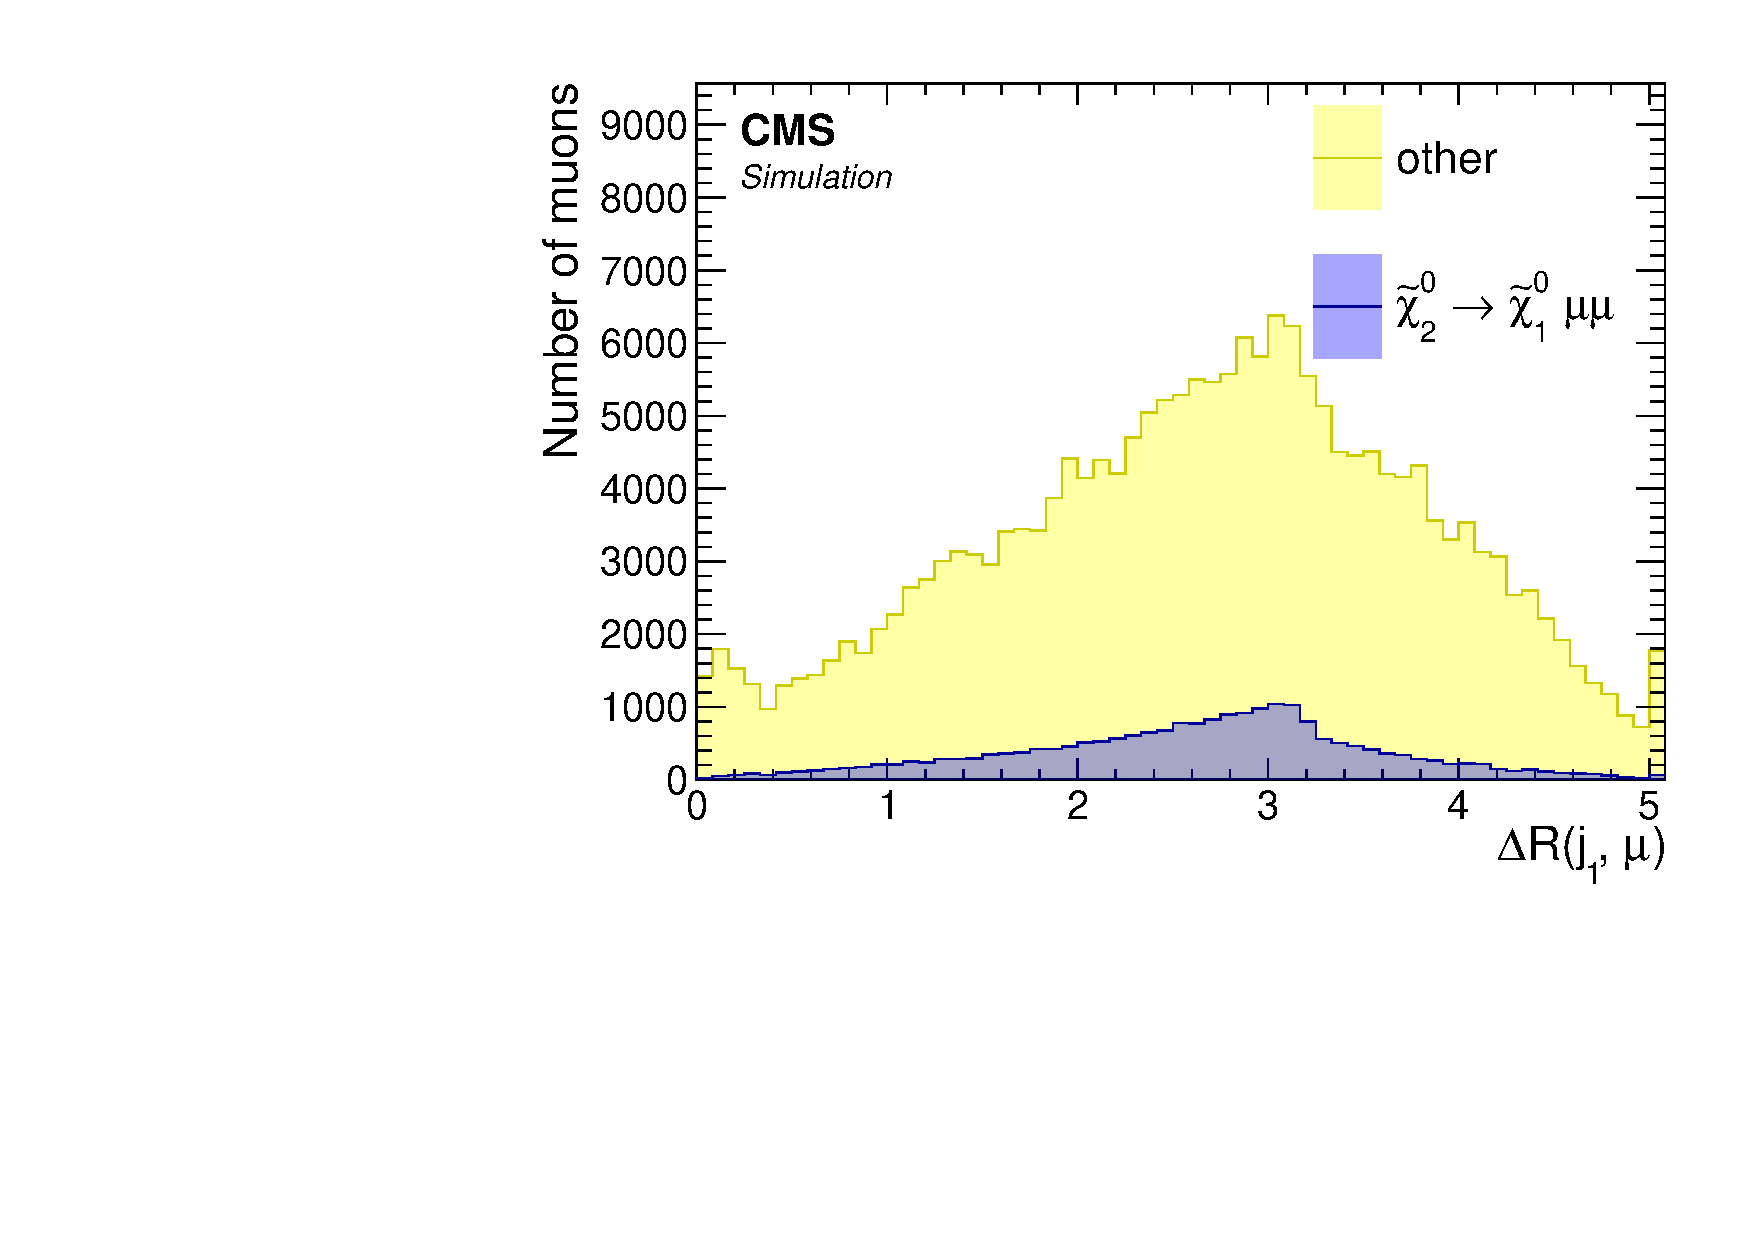
\includegraphics[width=0.32\linewidth]{plots/lepton_selection/lepton_selection_dm1p92/none_Muons_rlj.pdf} \,
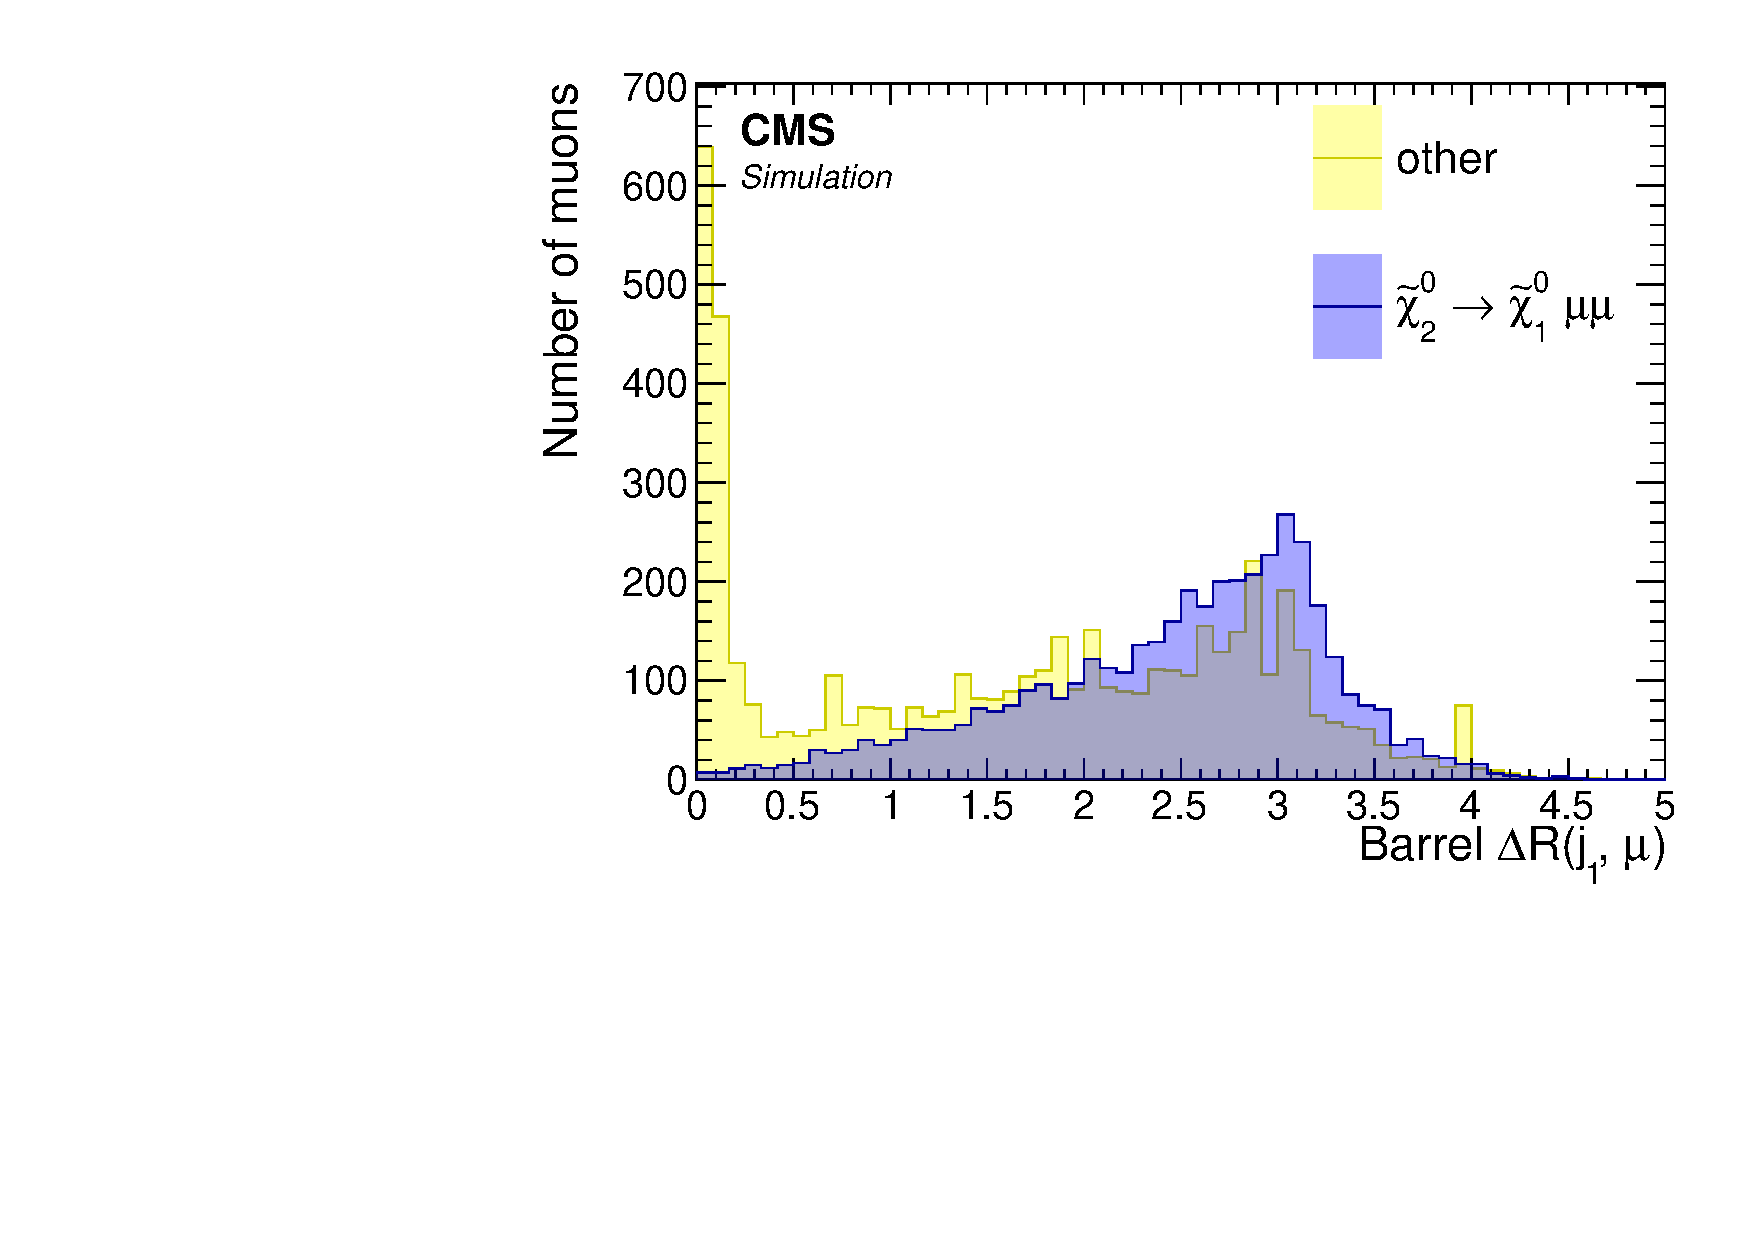
\includegraphics[width=0.32\linewidth]{plots/lepton_selection/lepton_selection_dm1p92/none_Muons_rlj_barrel.pdf}
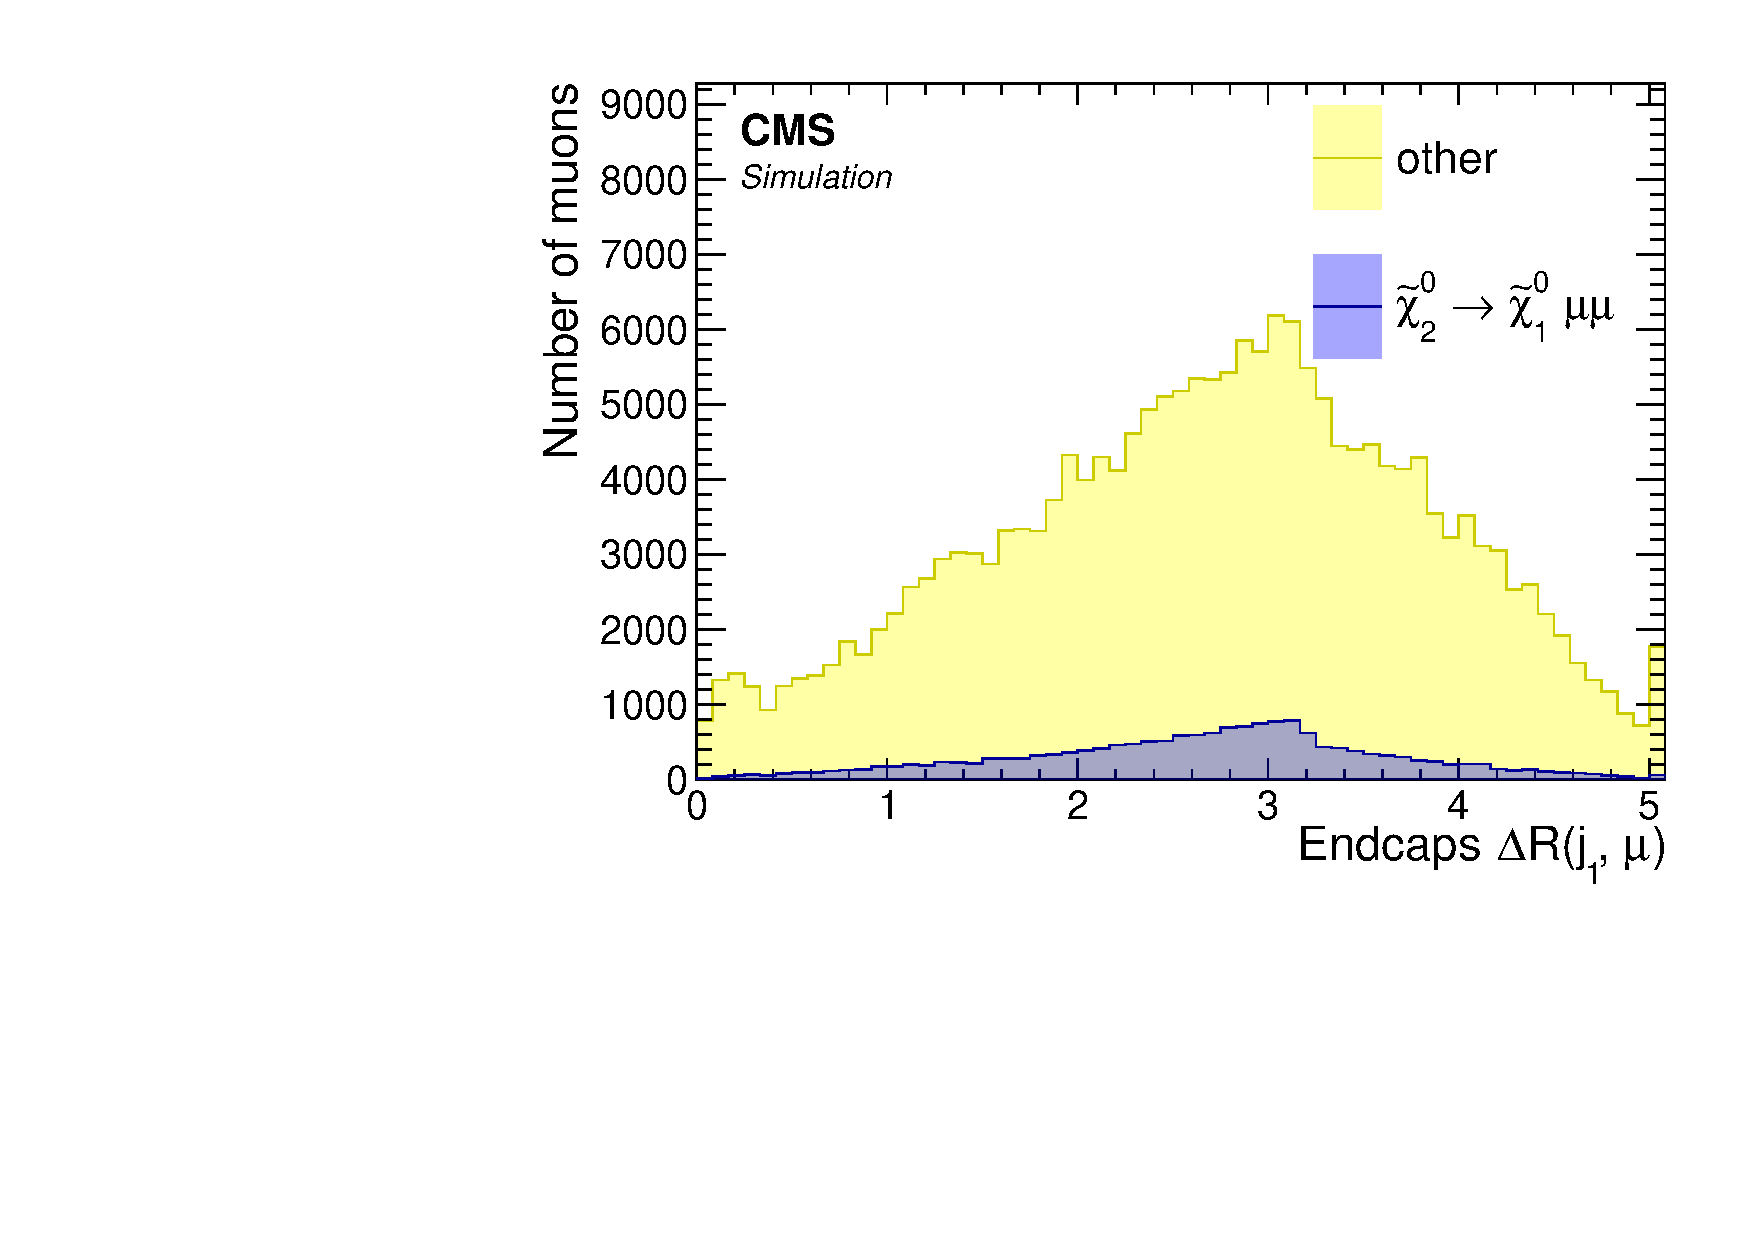
\includegraphics[width=0.32\linewidth]{plots/lepton_selection/lepton_selection_dm1p92/none_Muons_rlj_endcape.pdf}  \\
\caption[Angular separation between reconstructed muons and the leading jet $\DR(\jmath_1,\mu)$]{Angular separation between reconstructed muons with loose ID and the leading jet $\DR(\jmath_1,\mu)$ for $\dm=5.63\GeV$ (top) and $\dm=1.92\GeV$ (bottom) in the inclusive case (left), barrel (middle) and endcaps (right).}
\label{fig:muons-dr-lj}
\end{figure}

Distributions of muon \pt are examined having applied the previous cut of $\DR(\jmath_1,\mu)>0.4$. As seen in Section~\ref{sec:muon-eta-pt}, the \pt distribution depends strongly on $\dm$. The \pt distributions seen in Figure~\ref{fig:muons-selectrion-pt} suggest a cut identical to the electron case of $\pt<15\GeV$. It is worth mentioning that the \pt of the muons are included as input to the multivariate classifier employed at a later stage, which can effectively cut tighter on the \pt dynamically and in concert with cutting on other variables. The actual maximum value of the pT of the muons will depend on the \gls{bdt} cut being used to define the signal region. \pt of the muons will depend on the BDT cut being used to define the signal region. The feature discussed earlier, whereby the endcaps are capable of reconstructing muons with lower \pt and therefore have worse purity than the barrel, is reiterated here. It is important to stress that the worse purity is due to a much higher efficiency, and as long as the muons can be purified further, it is not necessarily a bad thing. The rate of  the non-signal muons in the region of $\pt<2\GeV$ is seen to diverge rapidly, and the ratio of signal muons to non-signal muons is very low in that region. Therefore, an additional cut of $\pt>2\GeV$ is adopted. To evaluate the effect of this cut, the $\abs{\eta}$ distribution before and after the \pt cut, is shown in Figure~\ref{fig:muons-selection-eta}.

\begin{figure}[!htb]
\centering
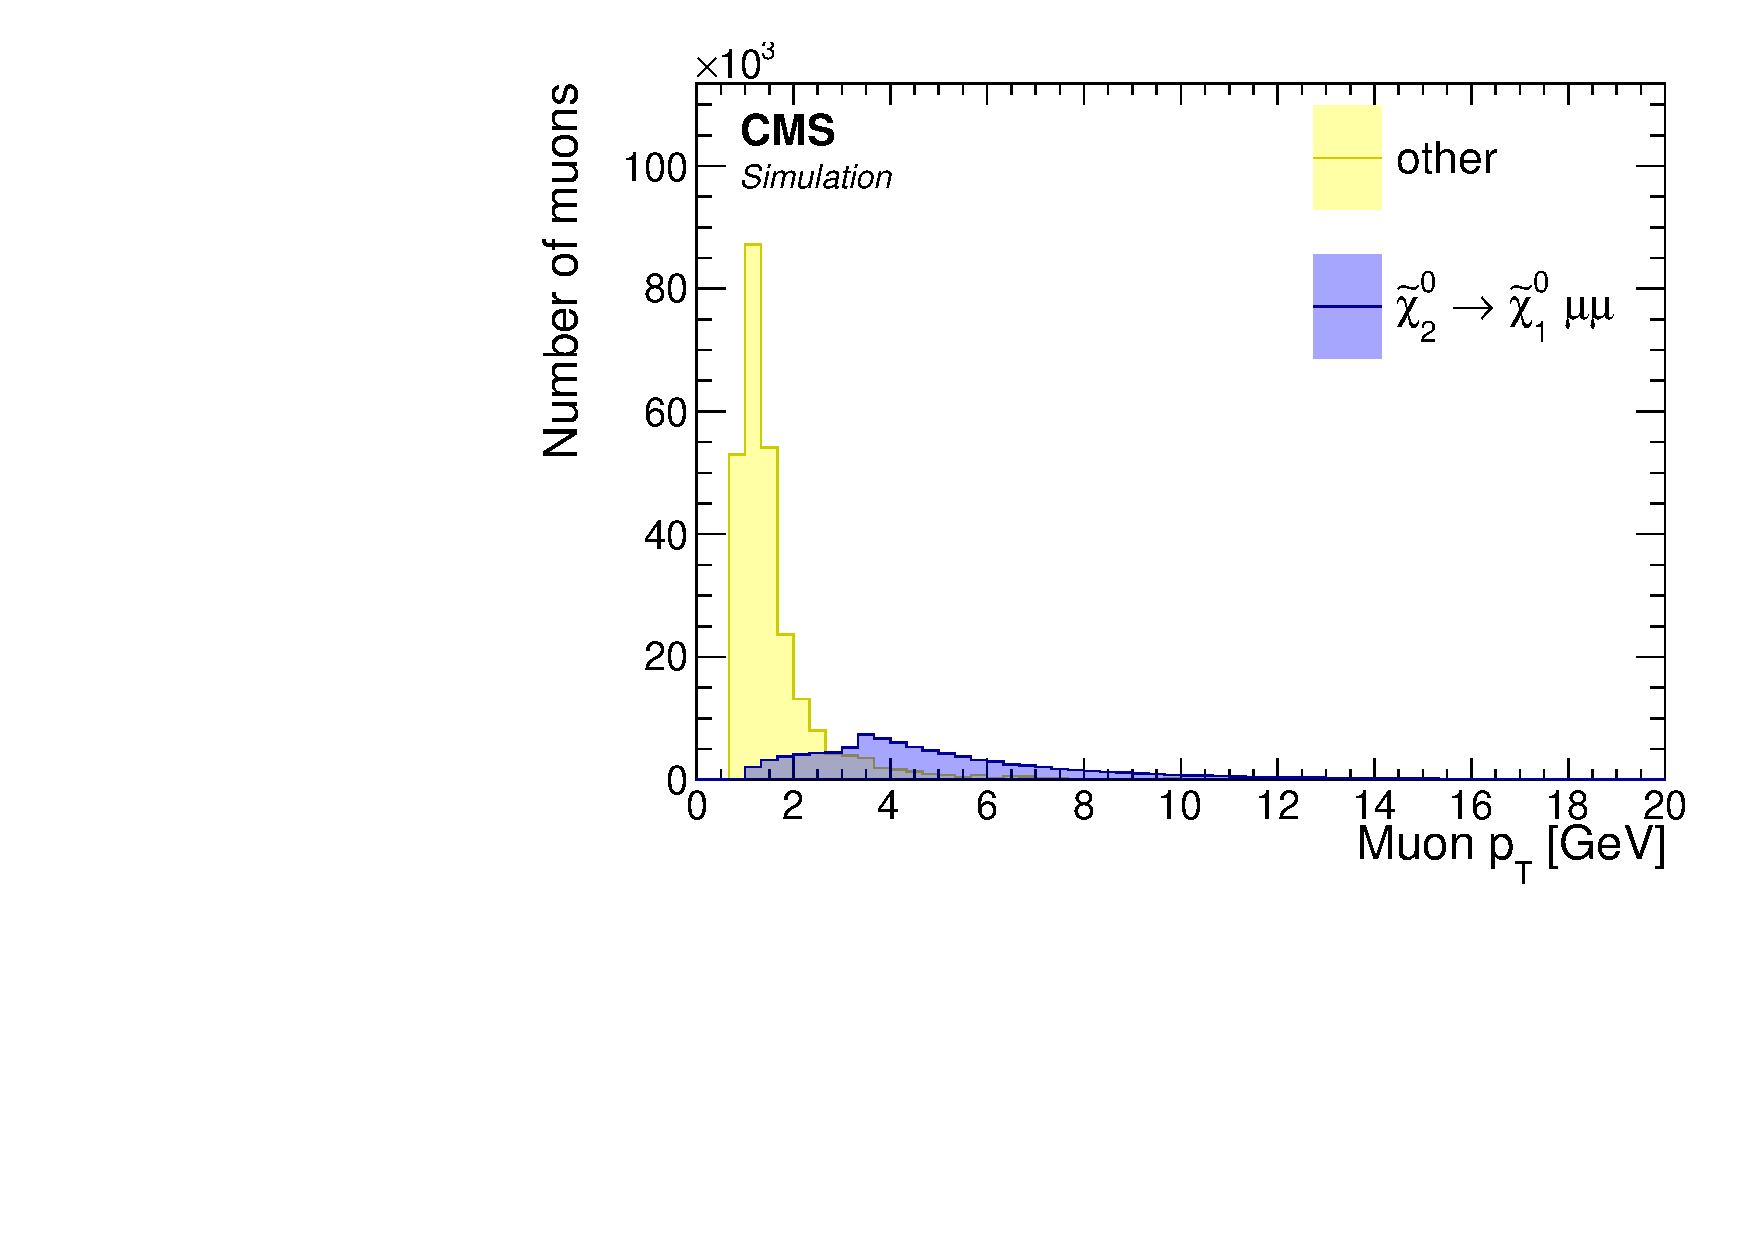
\includegraphics[width=0.32\linewidth]{plots/lepton_selection/lepton_selection_dm5p63/none_Muons_pt.pdf} \,
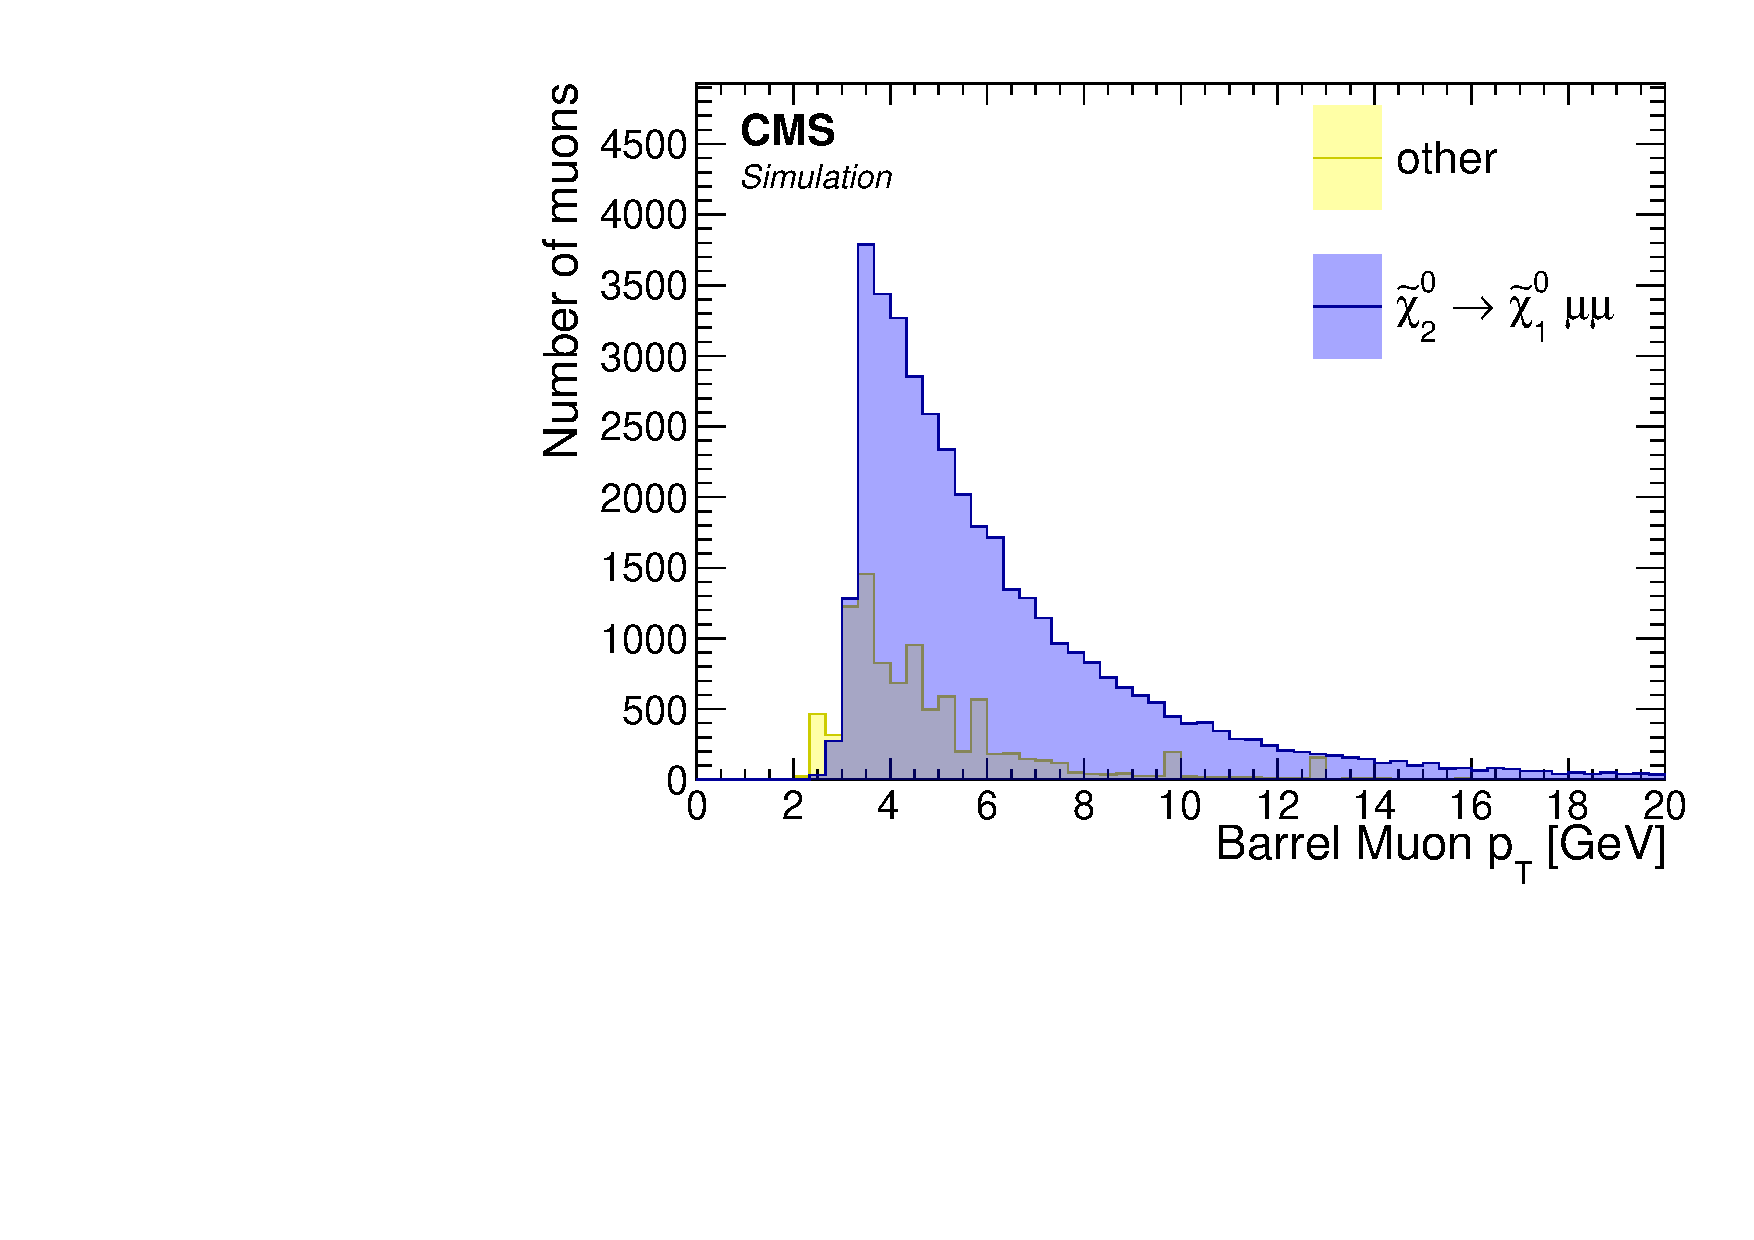
\includegraphics[width=0.32\linewidth]{plots/lepton_selection/lepton_selection_dm5p63/none_Muons_pt_barrel.pdf}
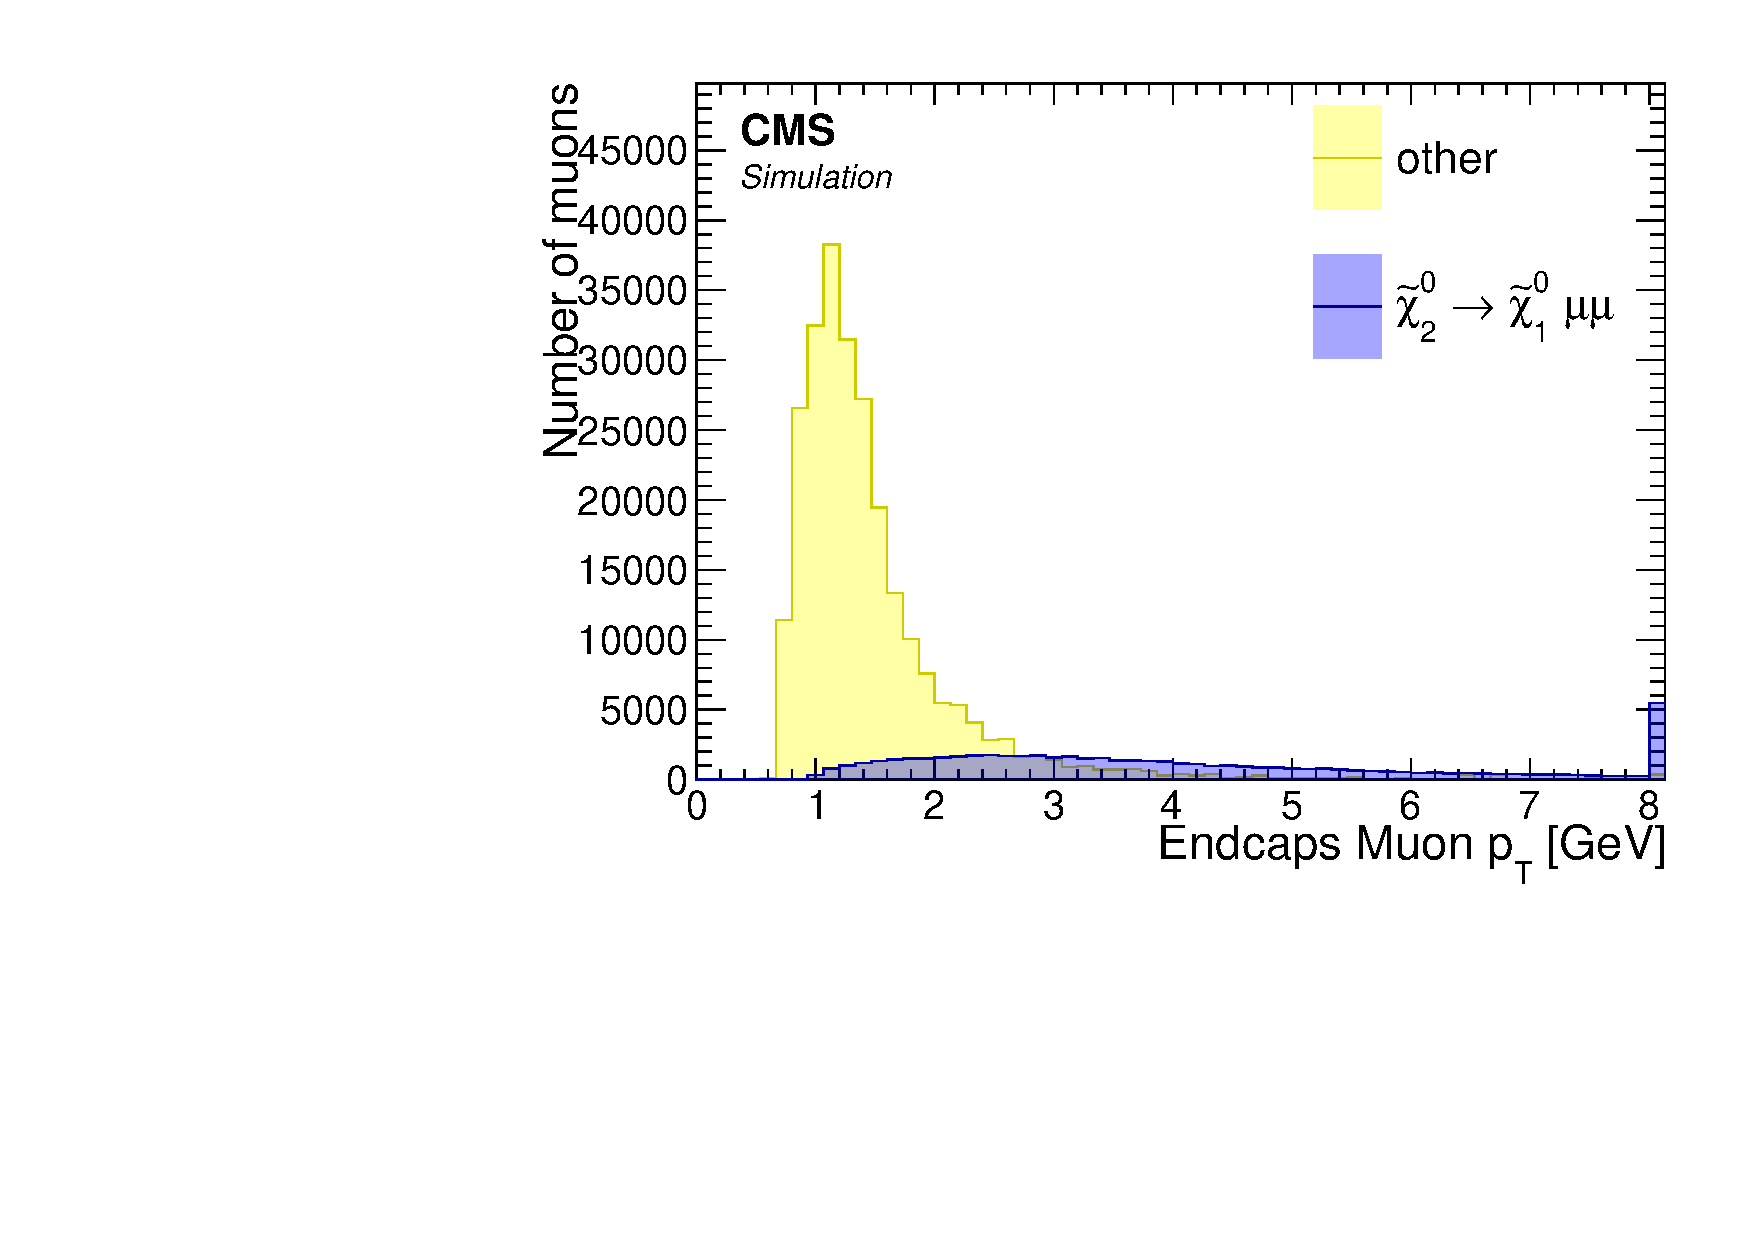
\includegraphics[width=0.32\linewidth]{plots/lepton_selection/lepton_selection_dm5p63/none_Muons_pt_endcape.pdf}  \\
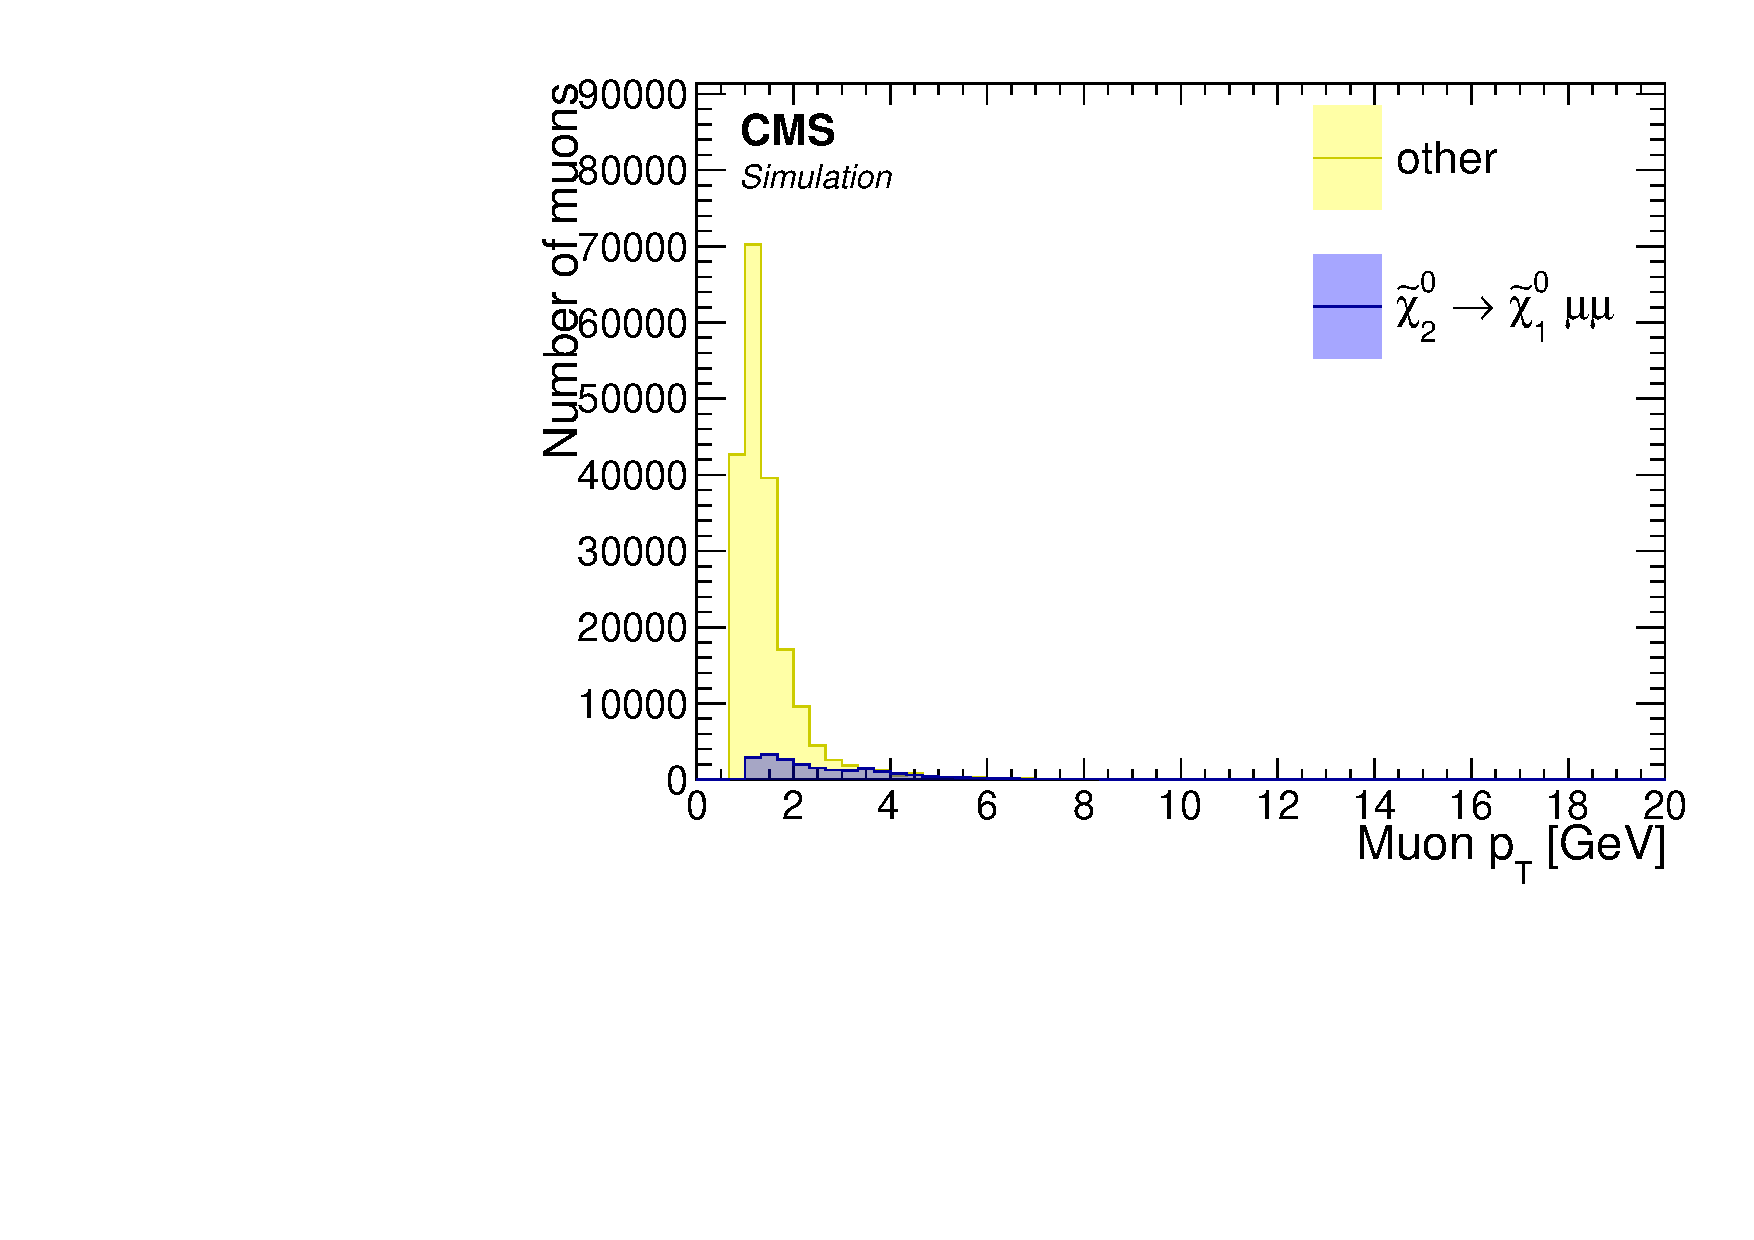
\includegraphics[width=0.32\linewidth]{plots/lepton_selection/lepton_selection_dm1p92/none_Muons_pt.pdf} \,
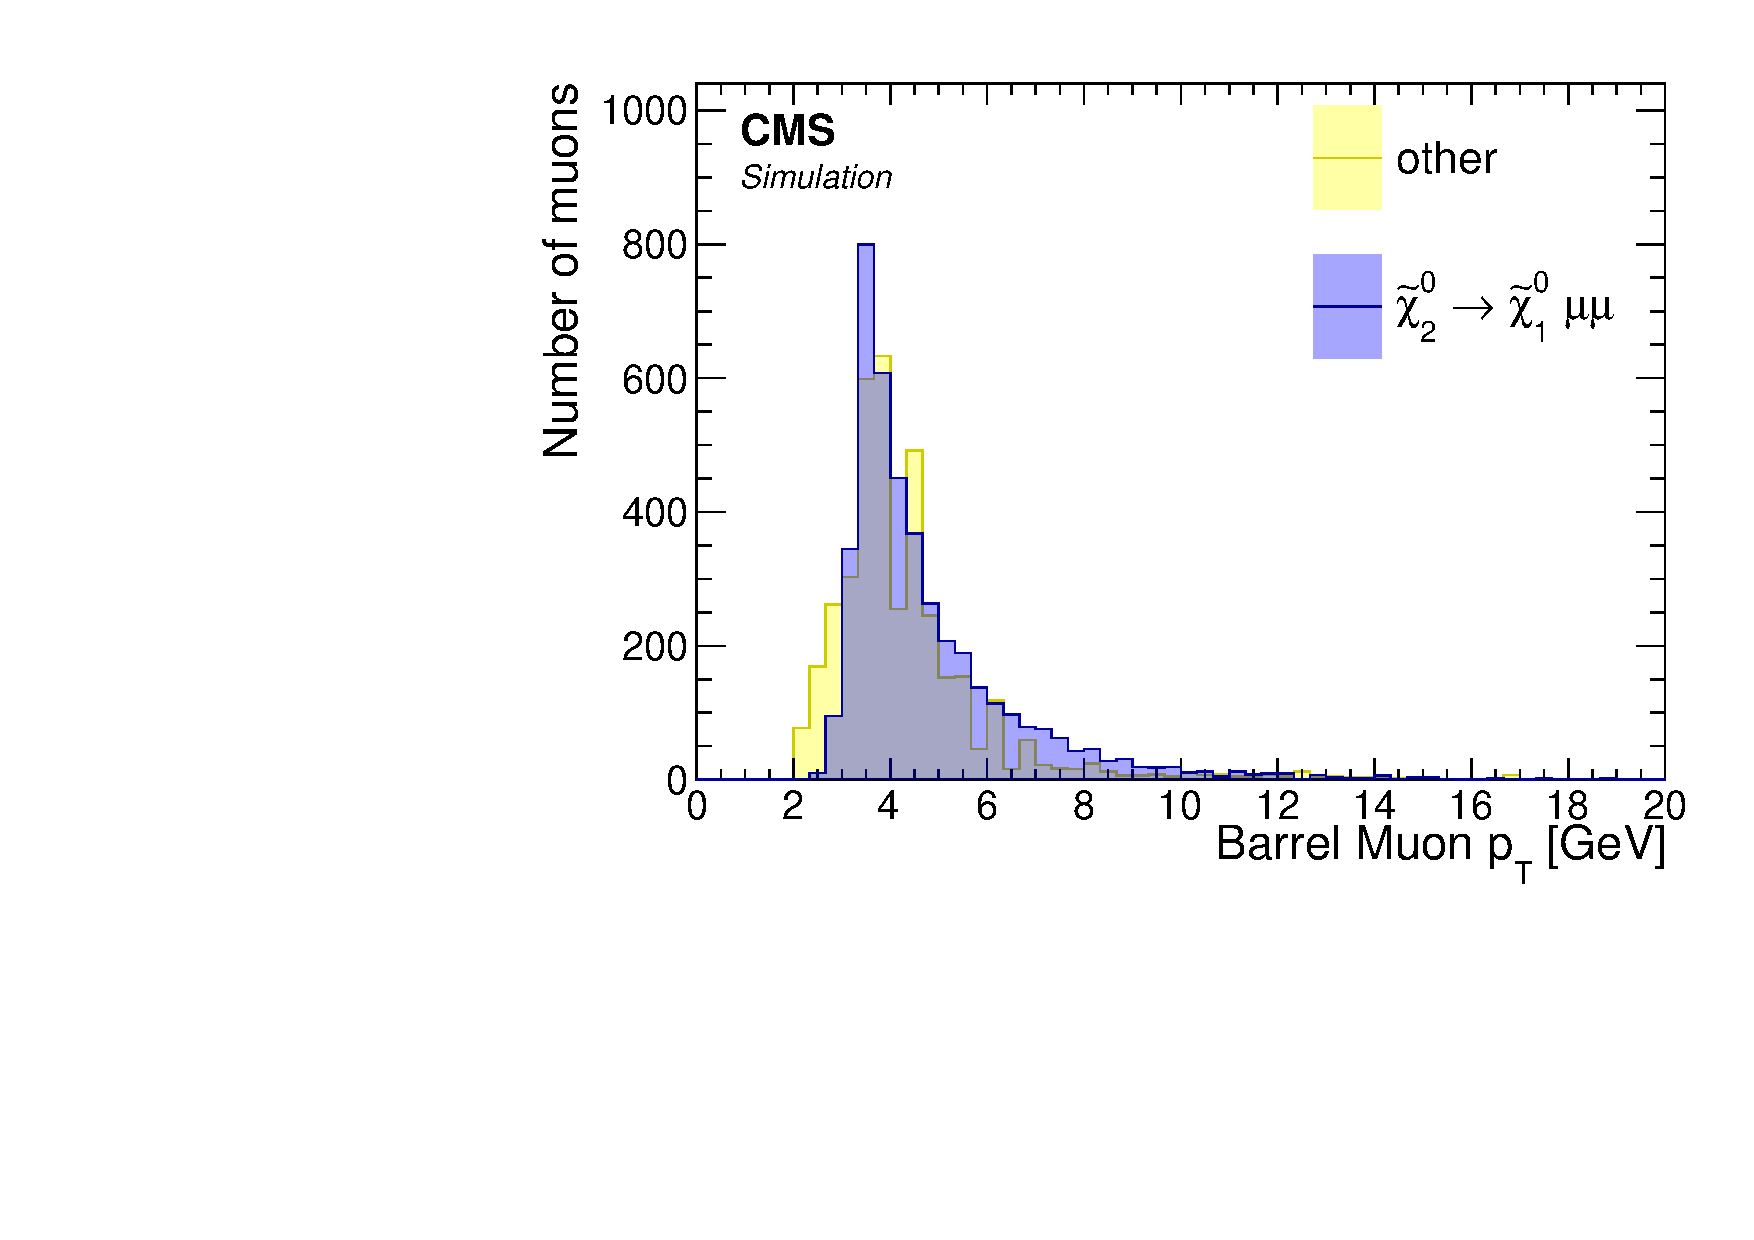
\includegraphics[width=0.32\linewidth]{plots/lepton_selection/lepton_selection_dm1p92/none_Muons_pt_barrel.pdf}
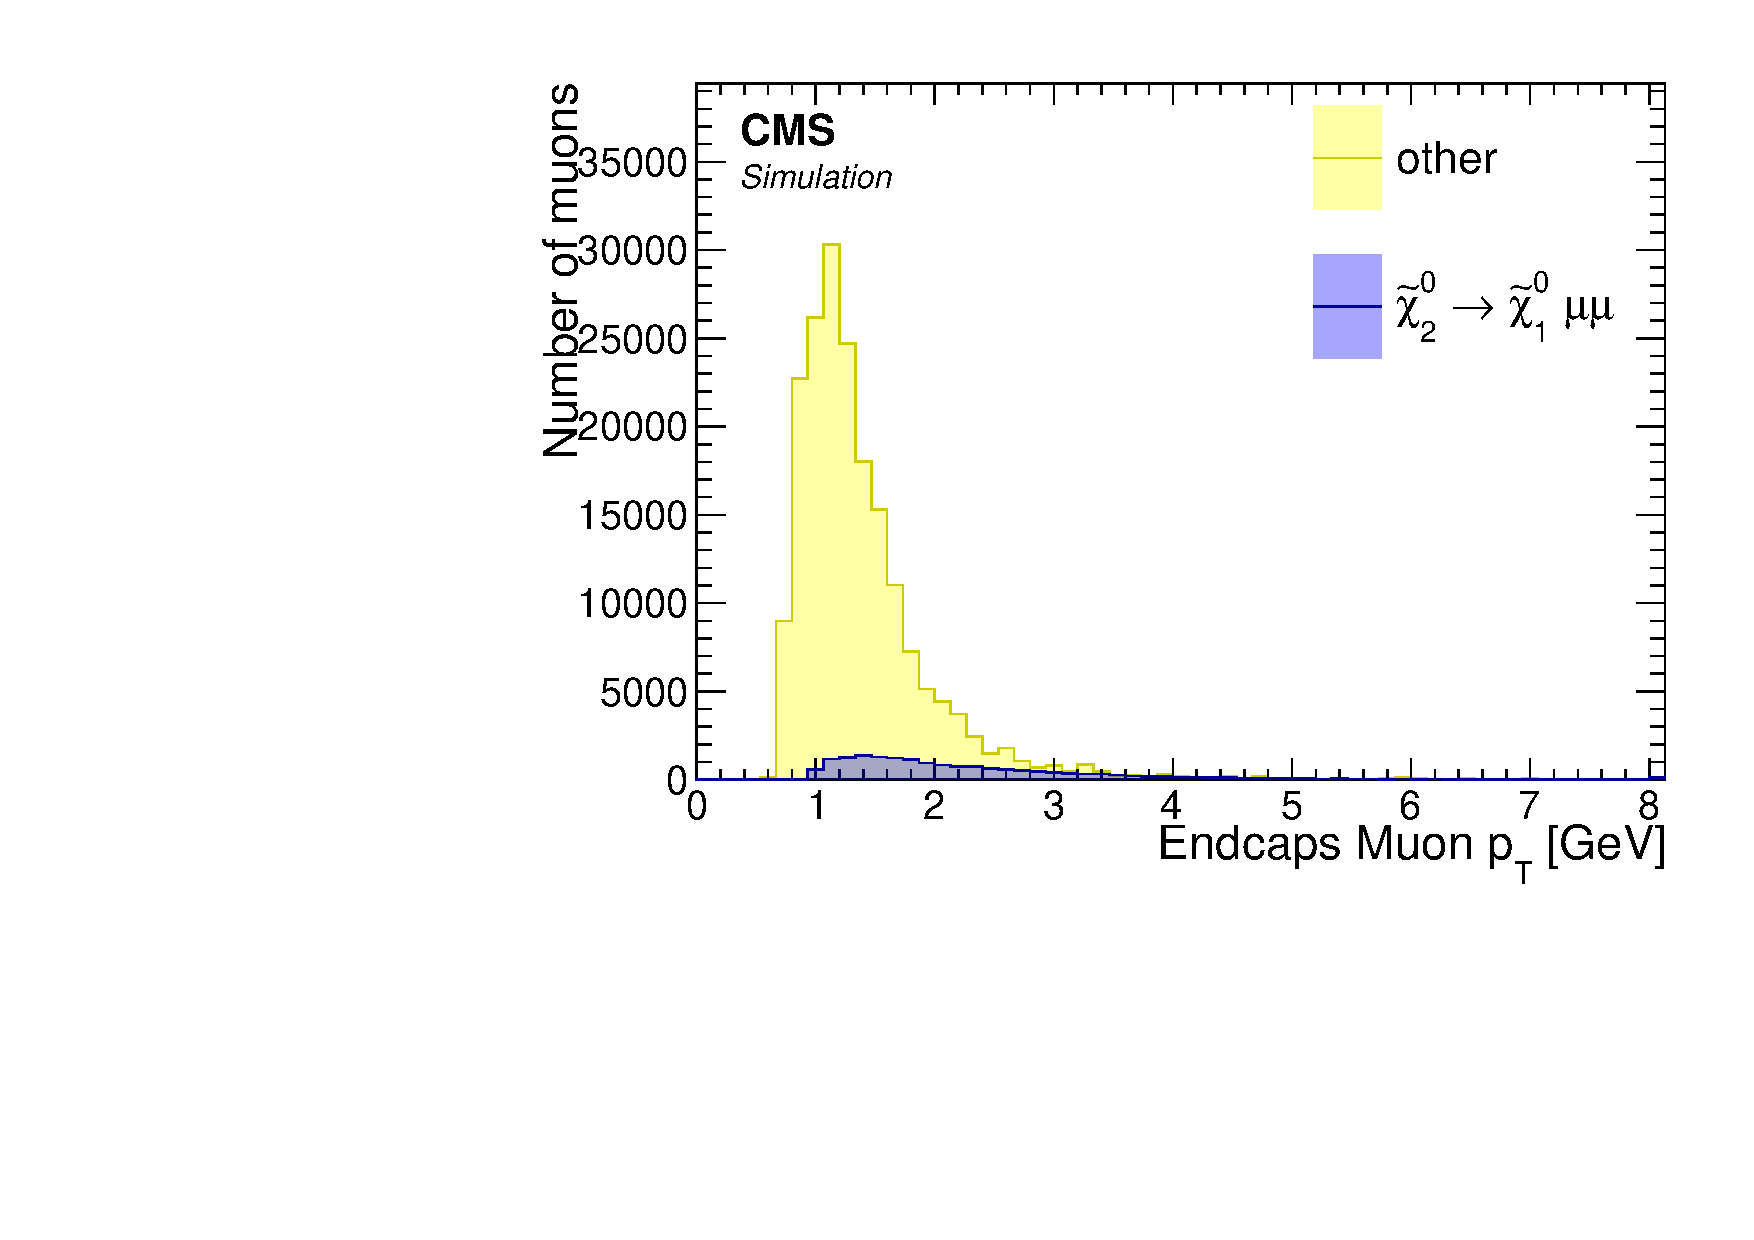
\includegraphics[width=0.32\linewidth]{plots/lepton_selection/lepton_selection_dm1p92/none_Muons_pt_endcape.pdf}  \\
\caption[Distibution in signal events of the $\pt$ of reconstructed muons]{Distibution in signal events of the $\pt$ of reconstructed muons with loose ID for $\dm=5.63\GeV$ (top) and $\dm=1.92\GeV$ (bottom) in the inclusive case (left), barrel (middle) and endcaps (right). Cuts of $\DR(\jmath_1,\mu)>0.4$ and $\pt<15\GeV$ are applied.}
\label{fig:muons-selectrion-pt}
\end{figure}

\begin{figure}[!htb]
\centering
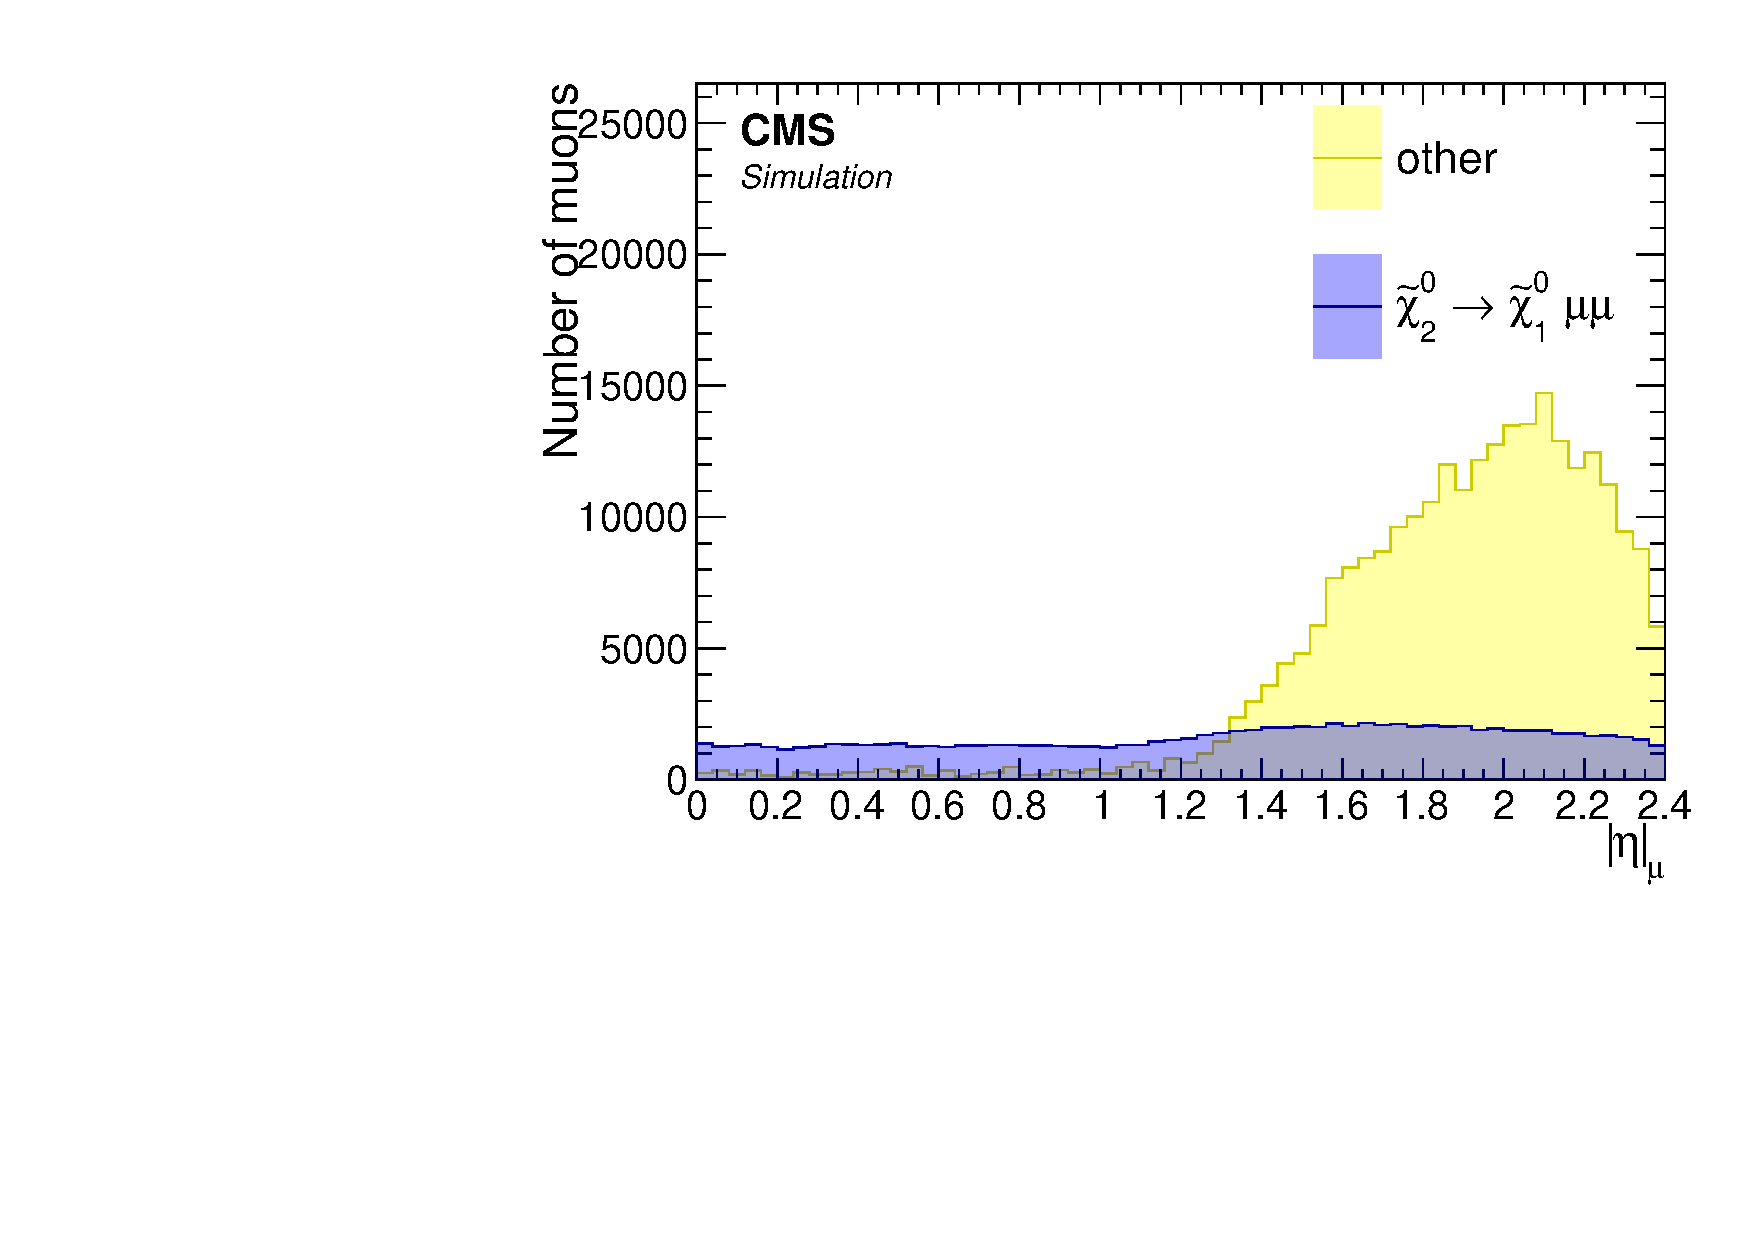
\includegraphics[width=0.48\linewidth]{plots/lepton_selection/lepton_selection_dm5p63/none_Muons_Eta.pdf} \,
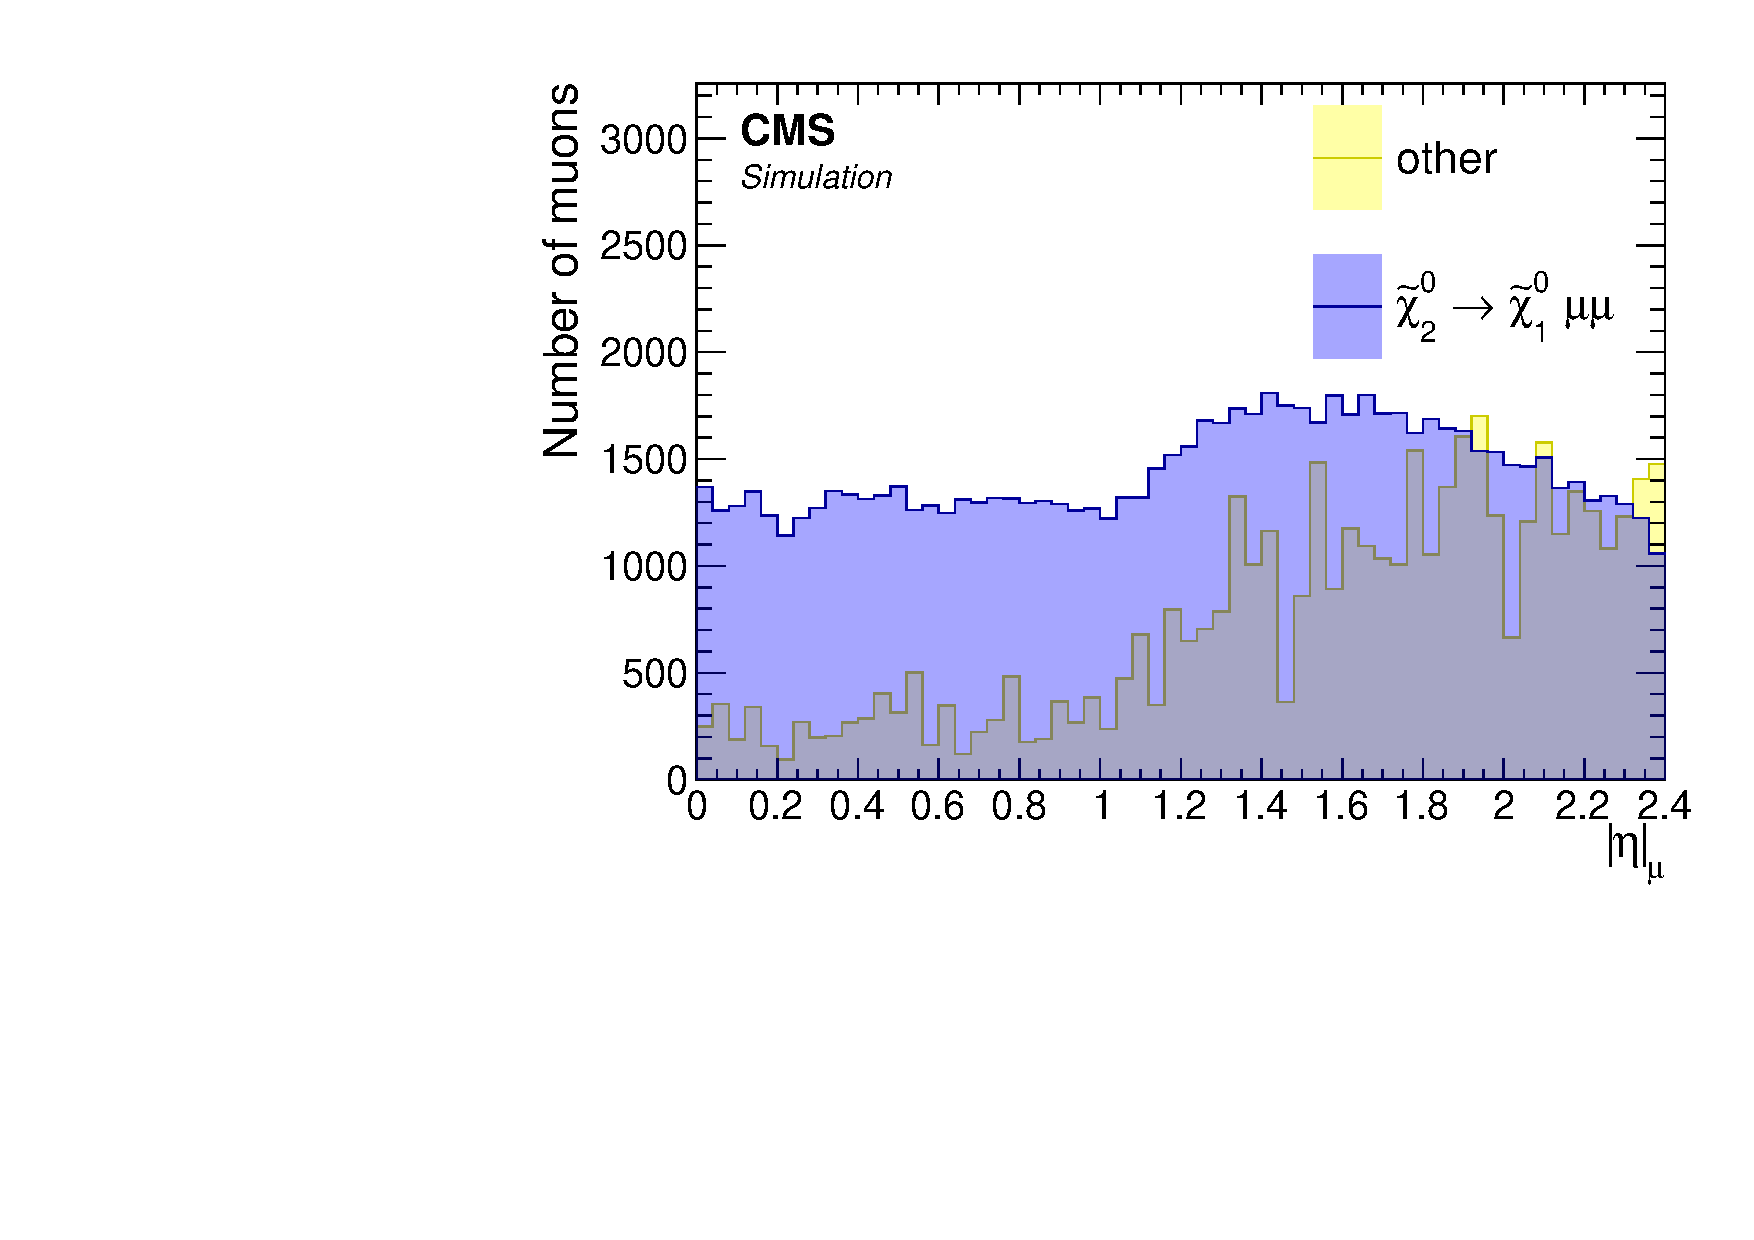
\includegraphics[width=0.48\linewidth]{plots/lepton_selection/lepton_selection_dm5p63/none_Muons_Eta_after_pt.pdf} \\
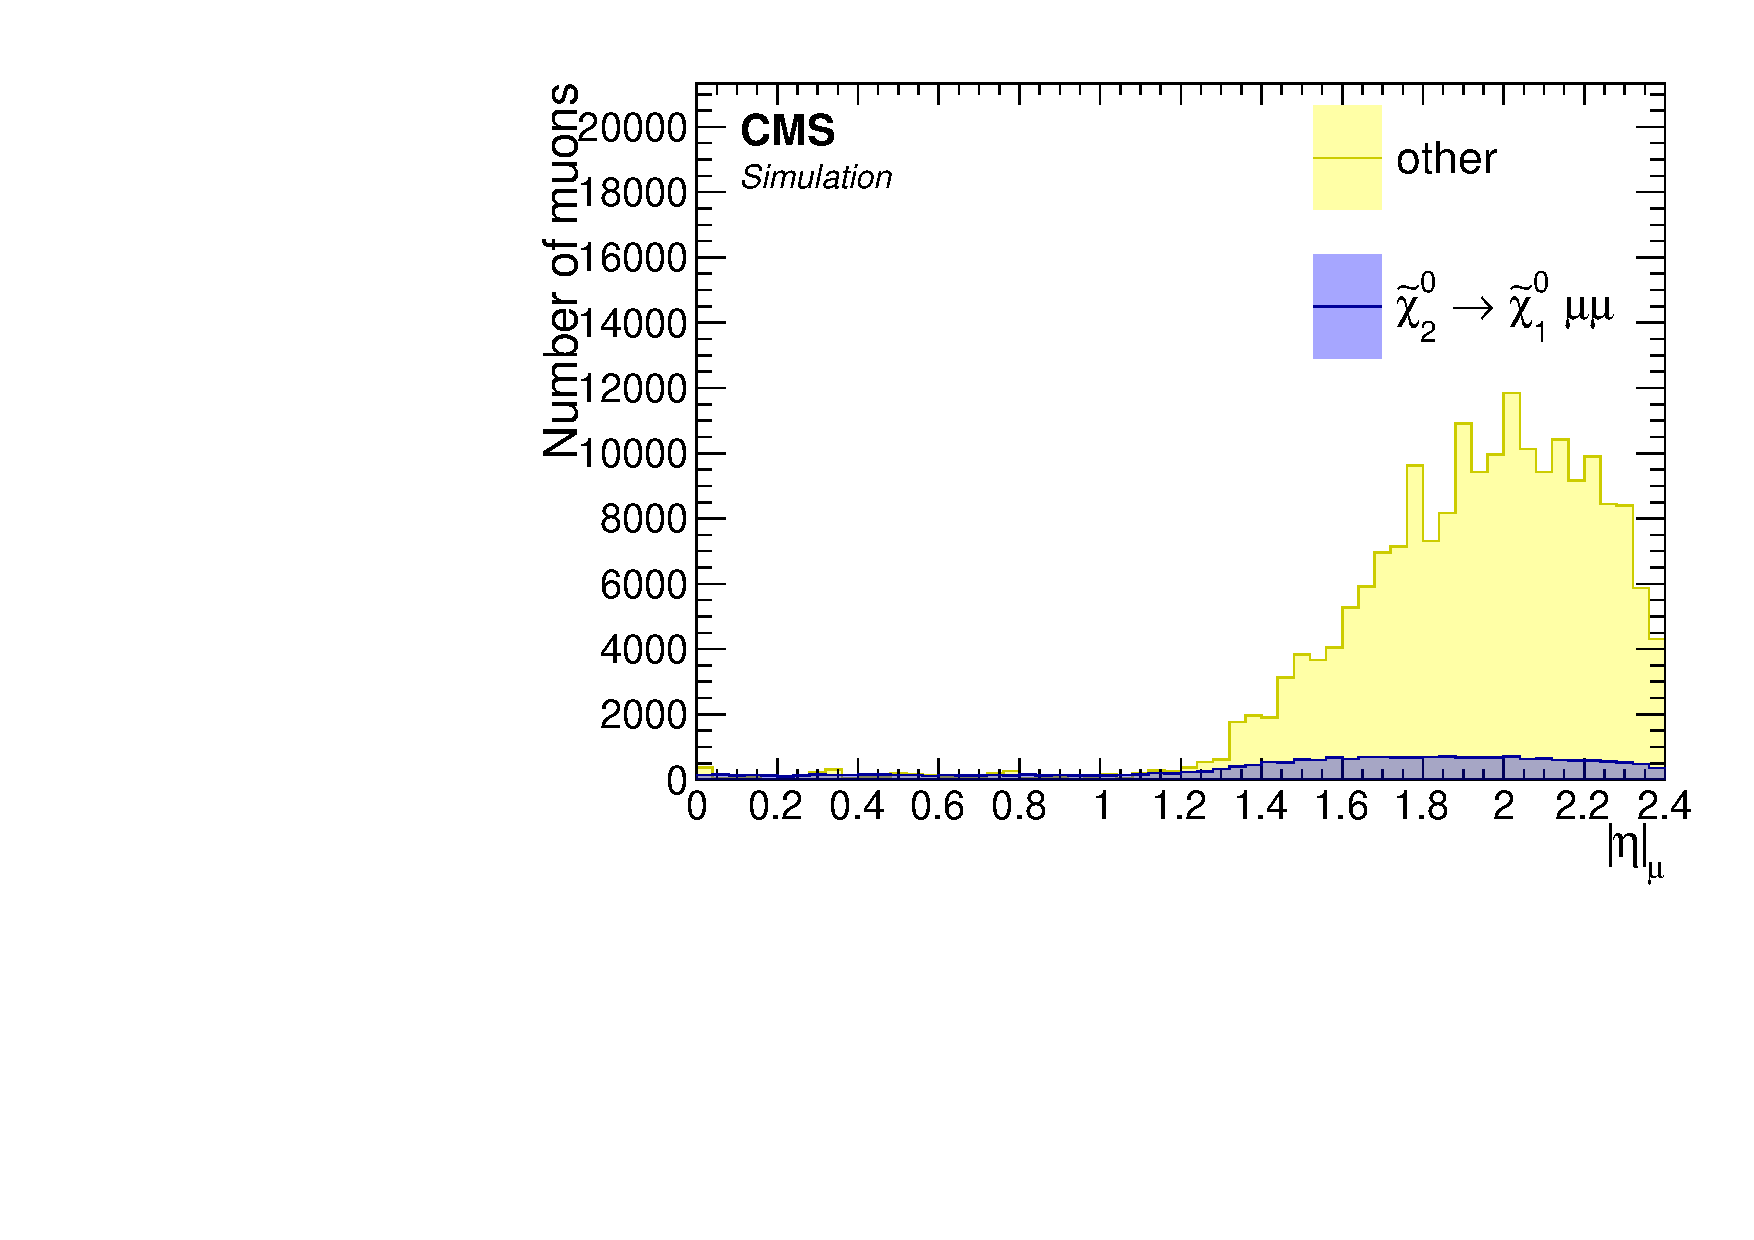
\includegraphics[width=0.48\linewidth]{plots/lepton_selection/lepton_selection_dm1p92/none_Muons_Eta.pdf}  \,
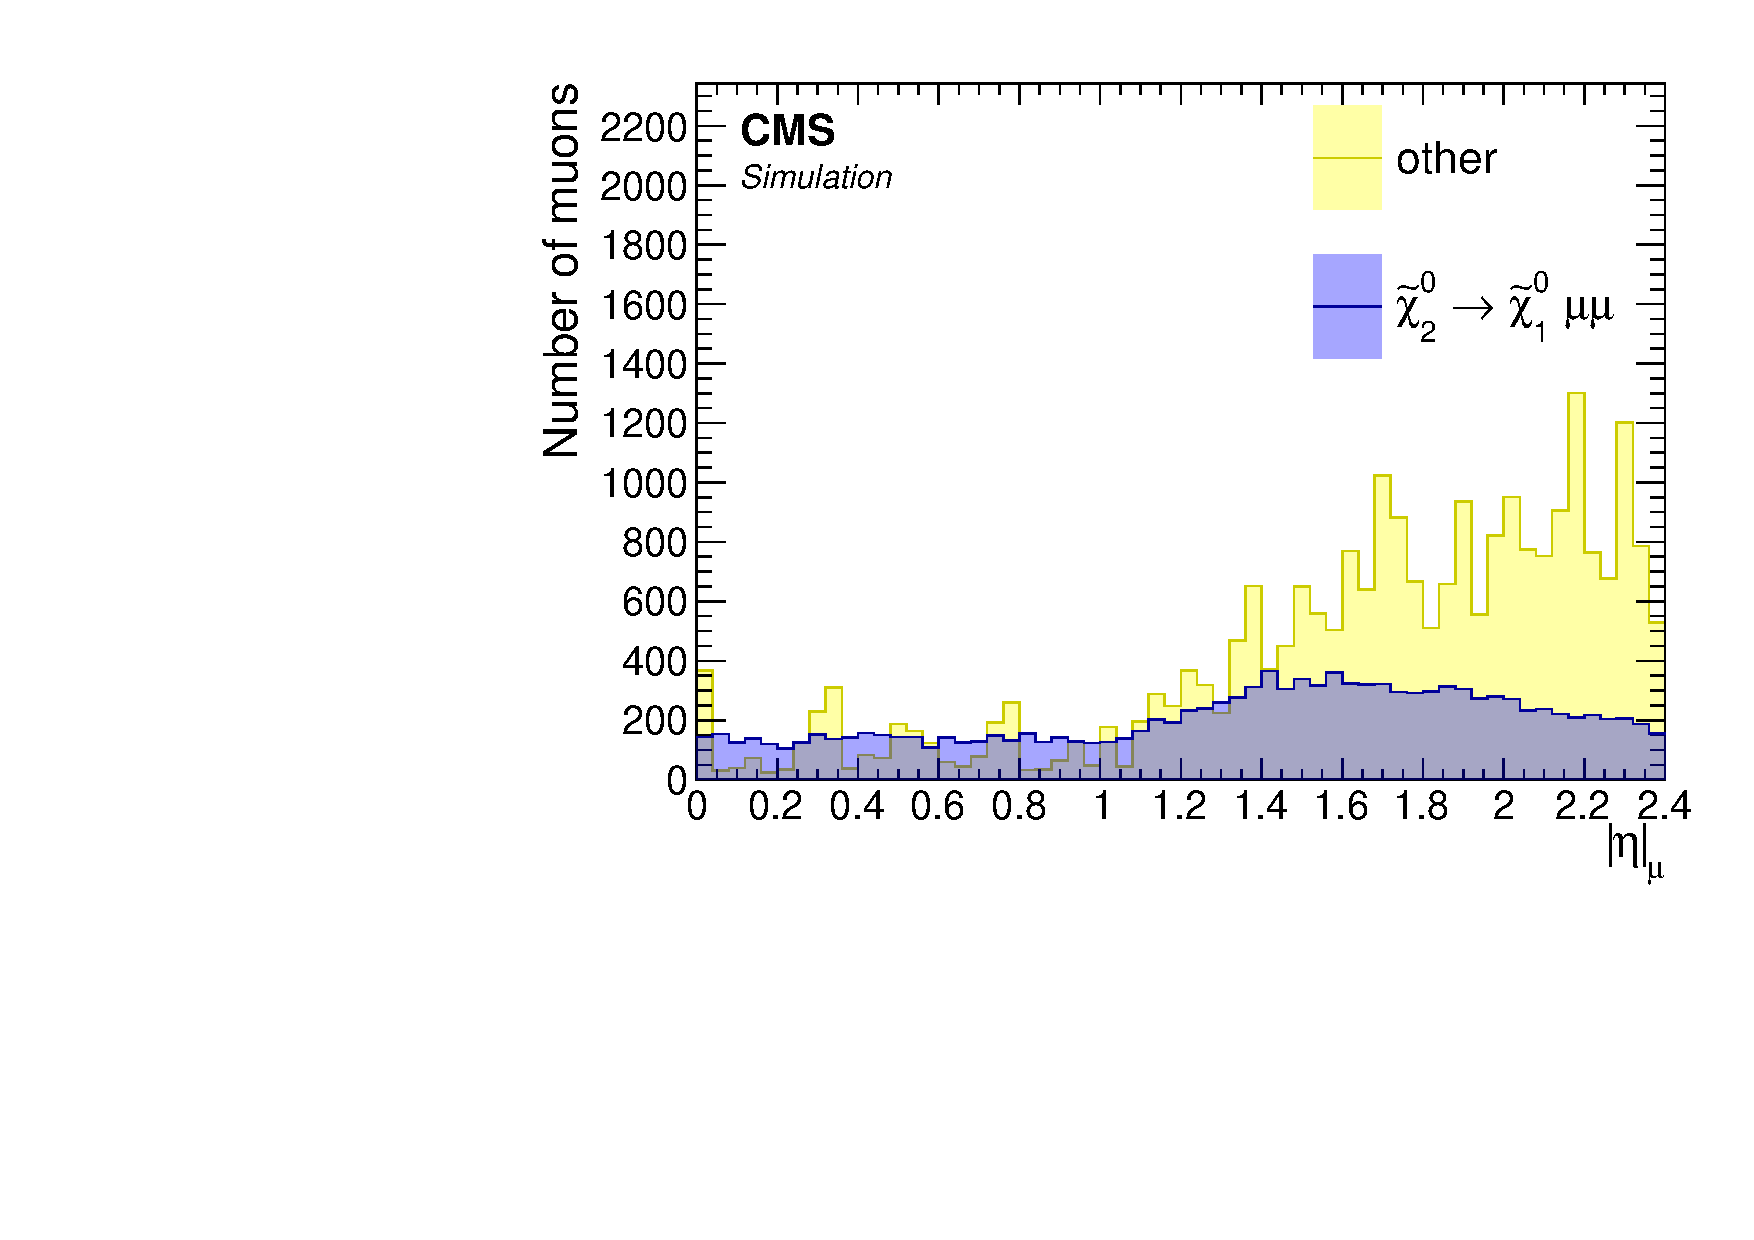
\includegraphics[width=0.48\linewidth]{plots/lepton_selection/lepton_selection_dm1p92/none_Muons_Eta_after_pt.pdf} \\
\caption[Distibution in signal events of the $\abs{\eta}$ of reconstructed muons with loose ID before and after $\pt>2\GeV$ cut]{Distibution in signal events of the $\abs{\eta}$ of reconstructed muons with loose ID for $\dm=5.63\GeV$ (top) and $\dm=1.92\GeV$ (bottom) without (left) and with (right) $\pt>2\GeV$ cut. A cut of $\DR(\jmath_1,\mu)>0.4$ is also applied.}
\label{fig:muons-selection-eta}
\end{figure}

The impact of choosing an alternate \gls{wp}, namely Medium or Tight, is examined in Figures~\ref{fig:muons-selection-id-medium} and~\ref{fig:muons-selection-id-tight}, respectively. Two bins labeled \emph{fail} and \emph{pass} are plotted, which correspond to whether the muon passes or fails the identification criteria of a Medium or Tight \glspl{wp}. The Medium \gls{wp} is seen to be highly performant in purifying the muon sample. The Tight \gls{wp} on the other hand leads to a significant number of wanted signal-muons being lost without a significant gain in purity. Therefore, the Medium ID \gls{wp} is chosen.

\begin{figure}[!htb]
\centering
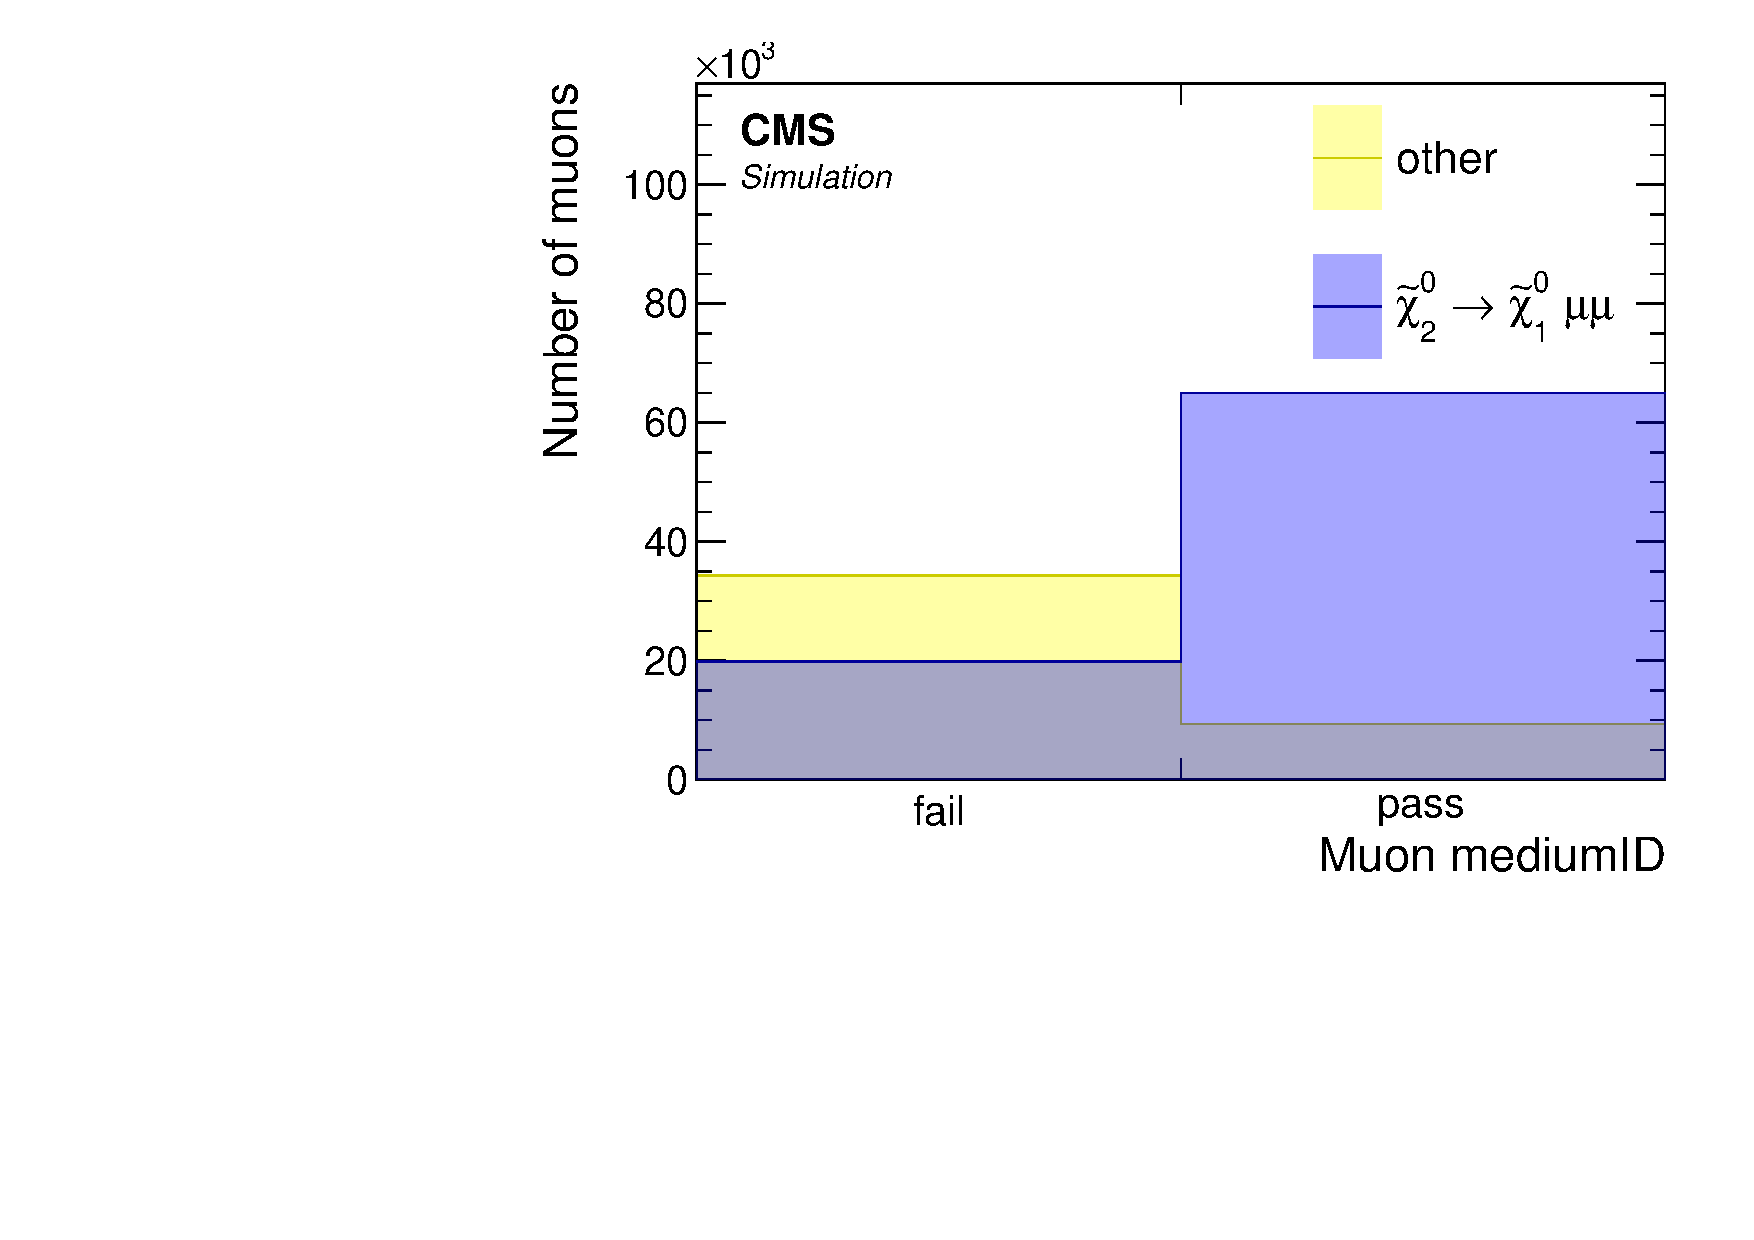
\includegraphics[width=0.32\linewidth]{plots/lepton_selection/lepton_selection_dm5p63/none_Muons_pt_medium.pdf} \,
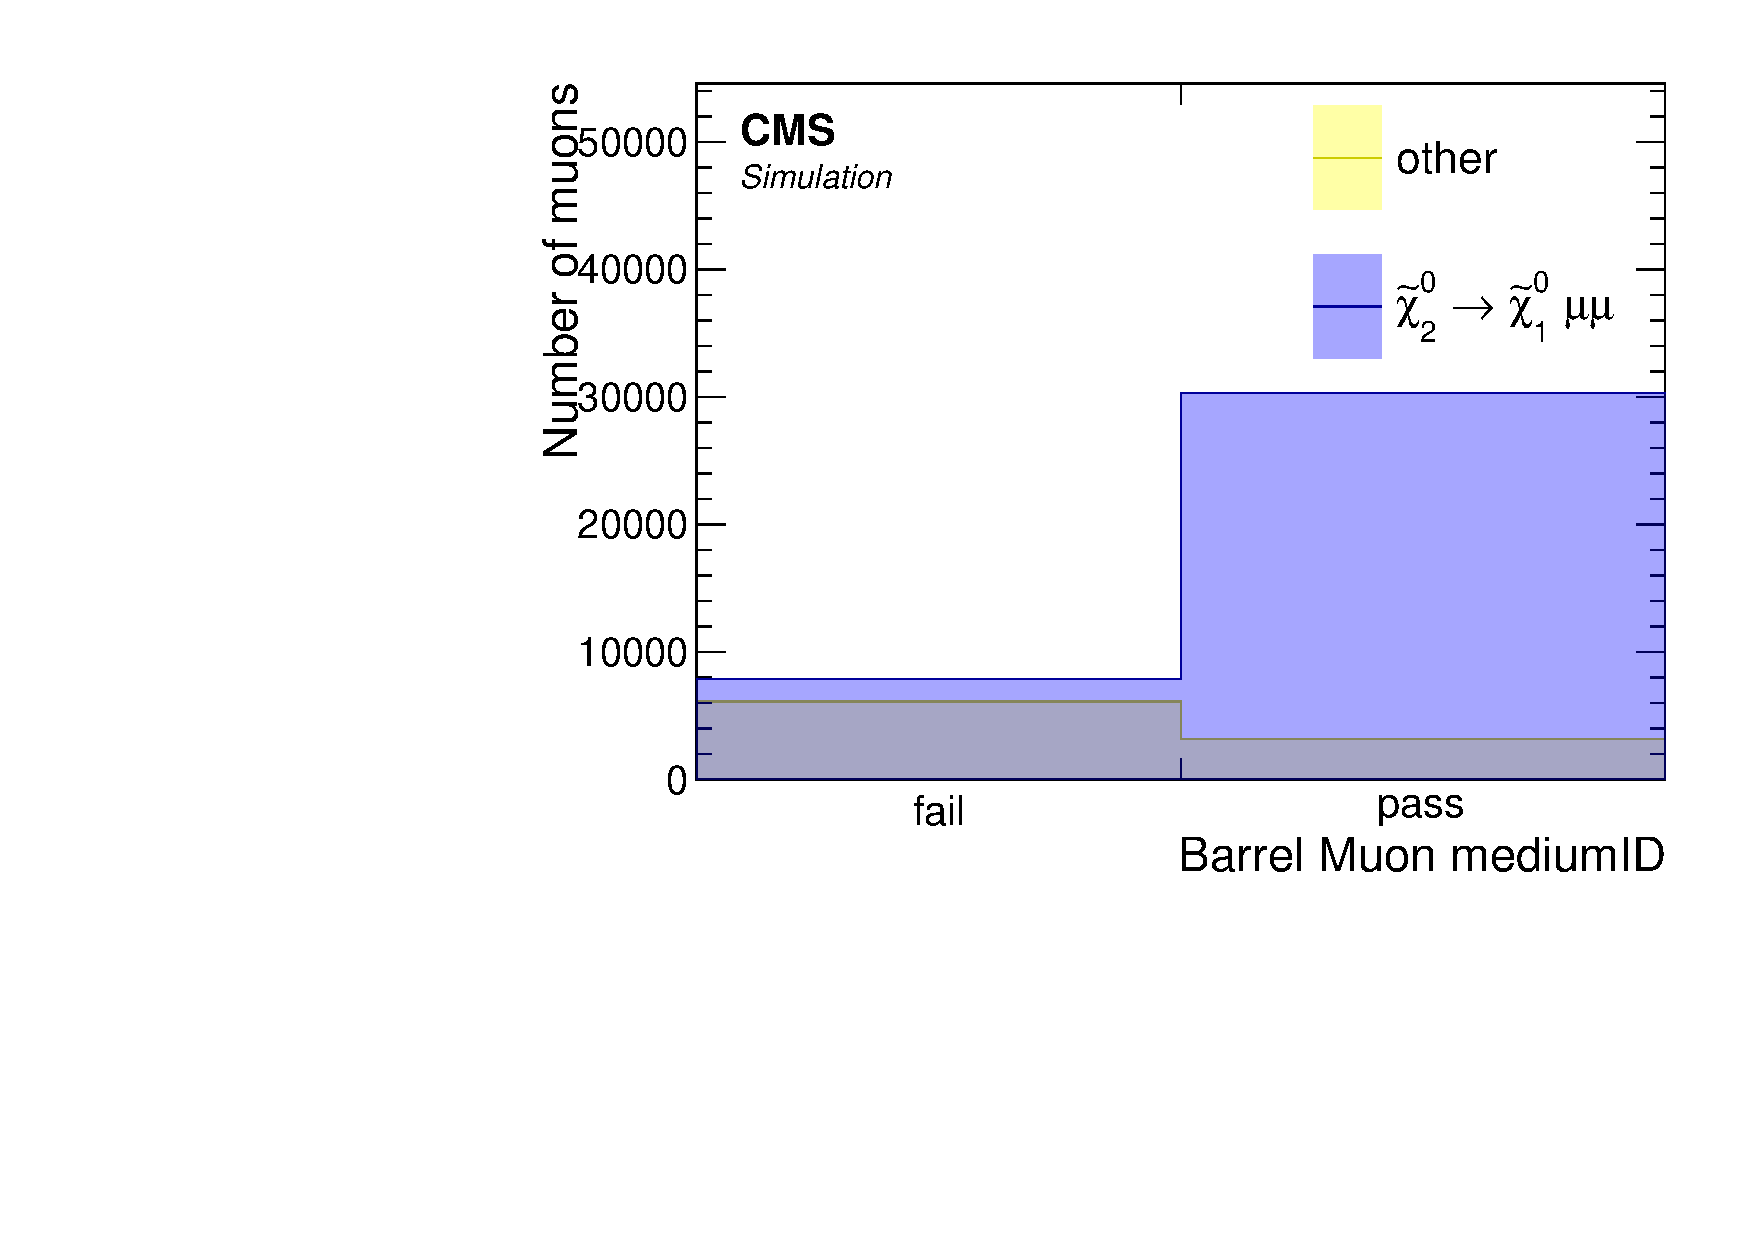
\includegraphics[width=0.32\linewidth]{plots/lepton_selection/lepton_selection_dm5p63/none_Muons_pt_barrel_medium.pdf} \,
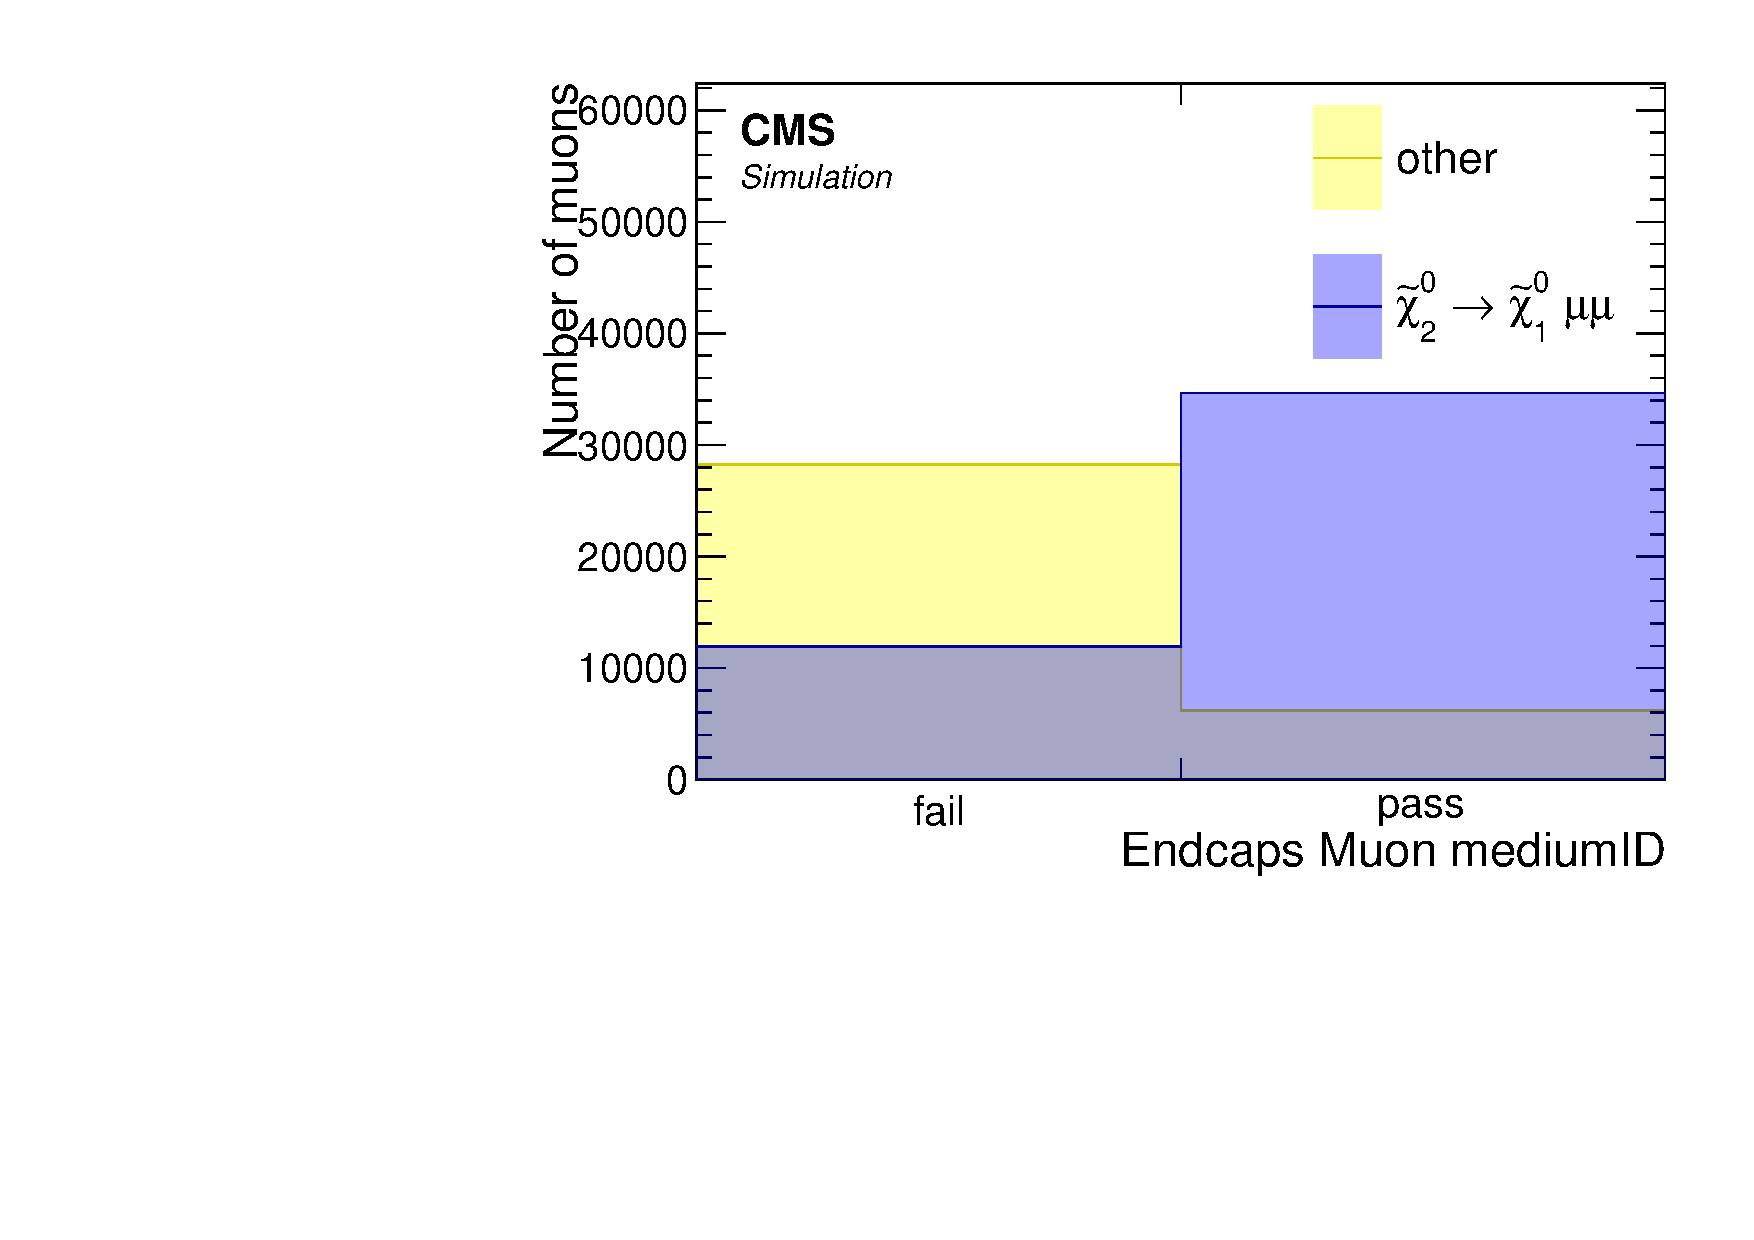
\includegraphics[width=0.32\linewidth]{plots/lepton_selection/lepton_selection_dm5p63/none_Muons_pt_endcape_medium.pdf}   \\
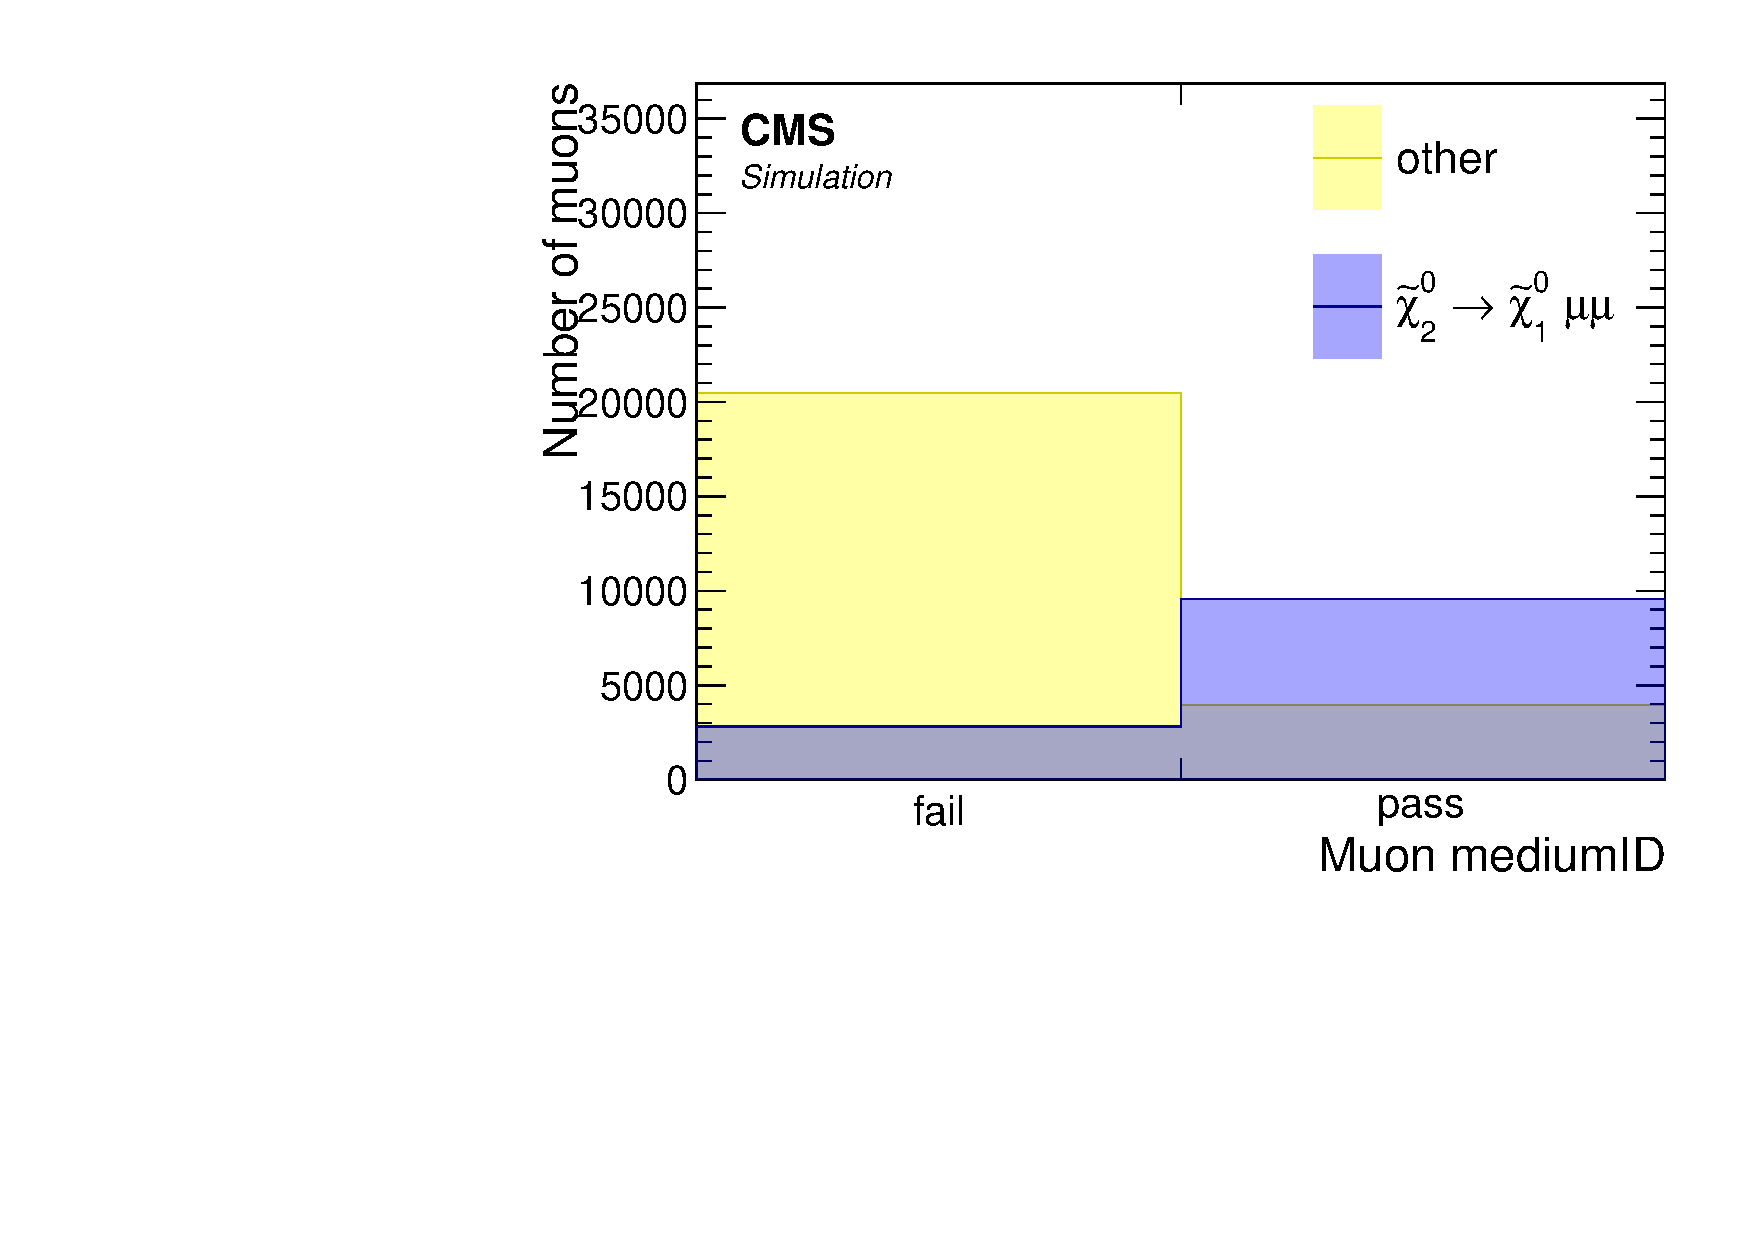
\includegraphics[width=0.32\linewidth]{plots/lepton_selection/lepton_selection_dm1p92/none_Muons_pt_medium.pdf} \,
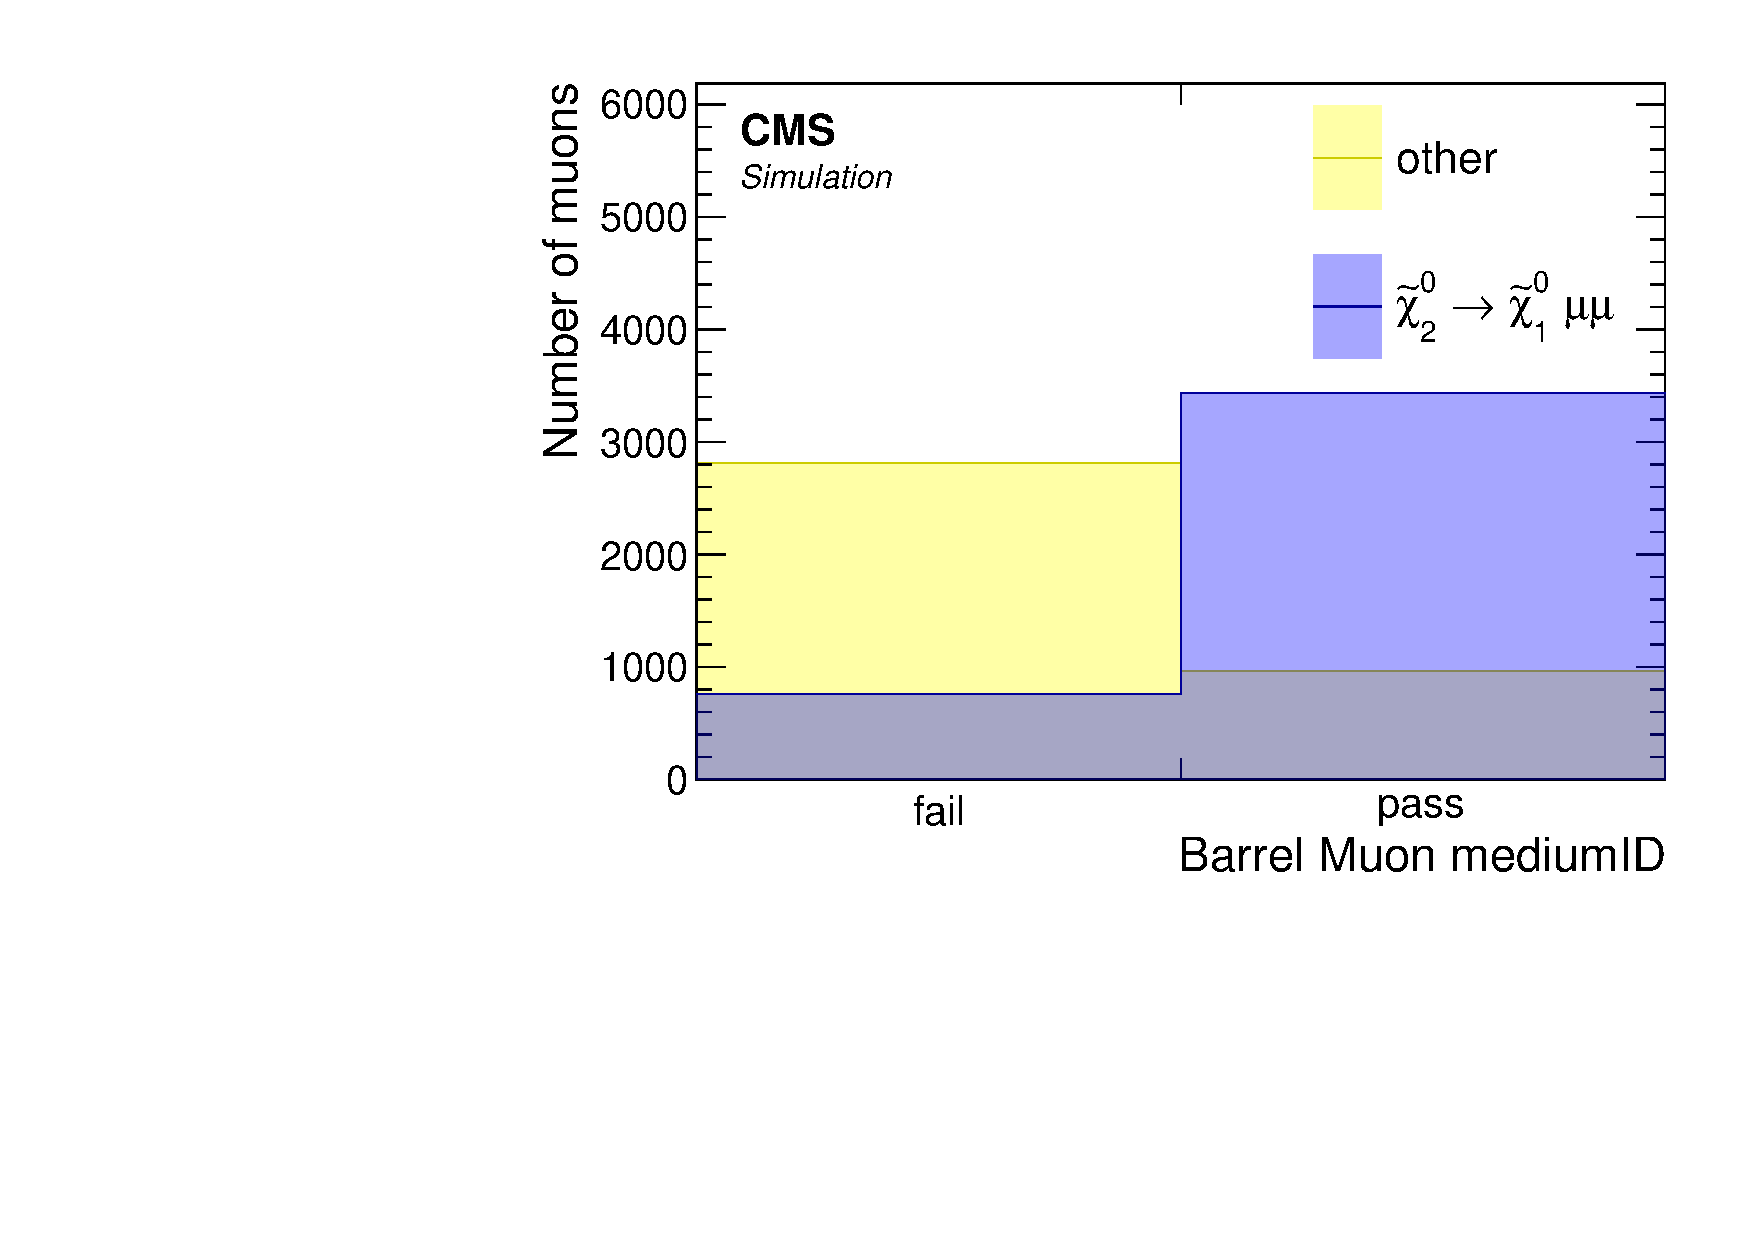
\includegraphics[width=0.32\linewidth]{plots/lepton_selection/lepton_selection_dm1p92/none_Muons_pt_barrel_medium.pdf}  \,
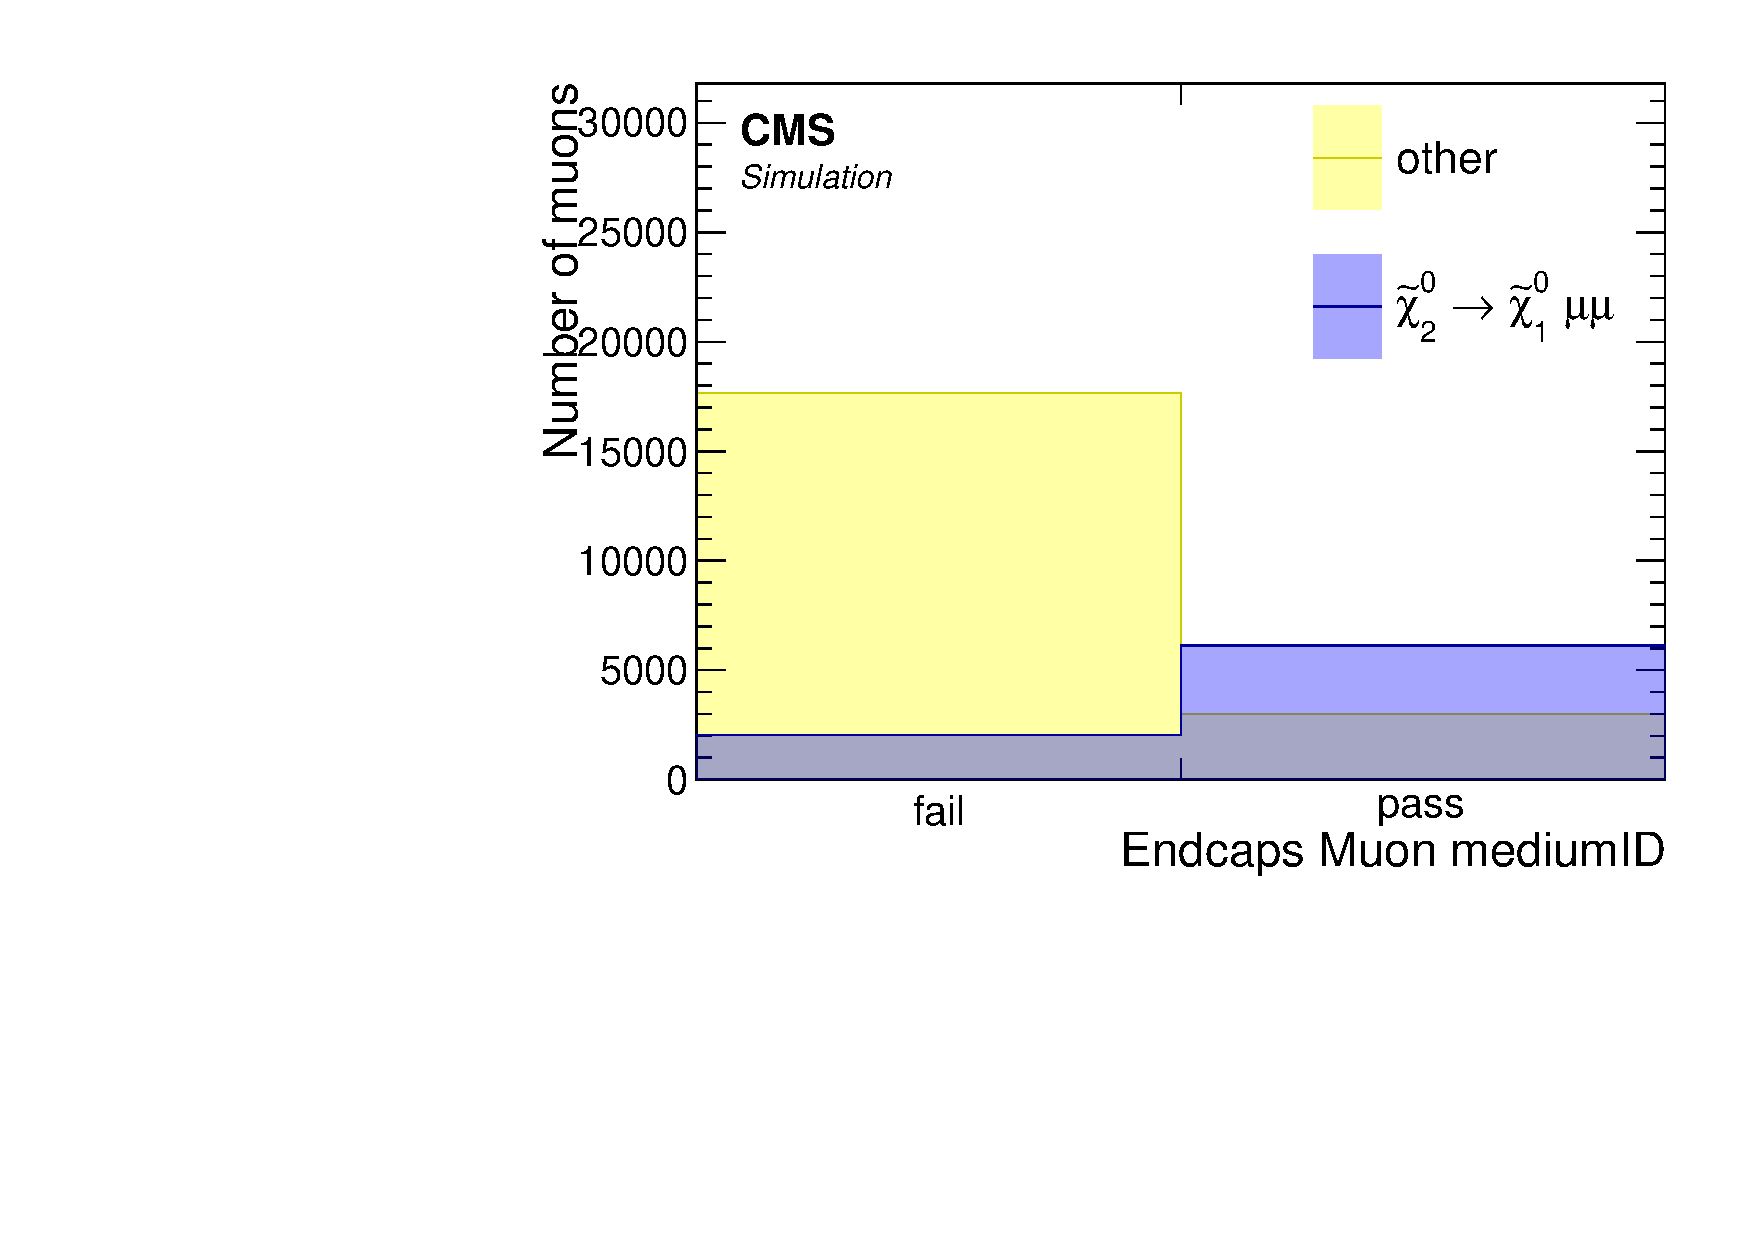
\includegraphics[width=0.32\linewidth]{plots/lepton_selection/lepton_selection_dm1p92/none_Muons_pt_endcape_medium.pdf} \\
\caption[Medium ID \gls{wp} distribution of reconstructed muons]{Medium ID \gls{wp} distributions of reconstructed muons for $\dm=5.63\GeV$ (top) and $\dm=1.92\GeV$ (bottom) in the inclusive $\pt$ case (left), barrel (middle) and endcaps (right). Cuts of $\DR(\jmath_1,\mu)>0.4$, $\pt>2\GeV$ and $\pt<15\GeV$ are applied.}
\label{fig:muons-selection-id-medium}
\end{figure}

\begin{figure}[!htb]
\centering
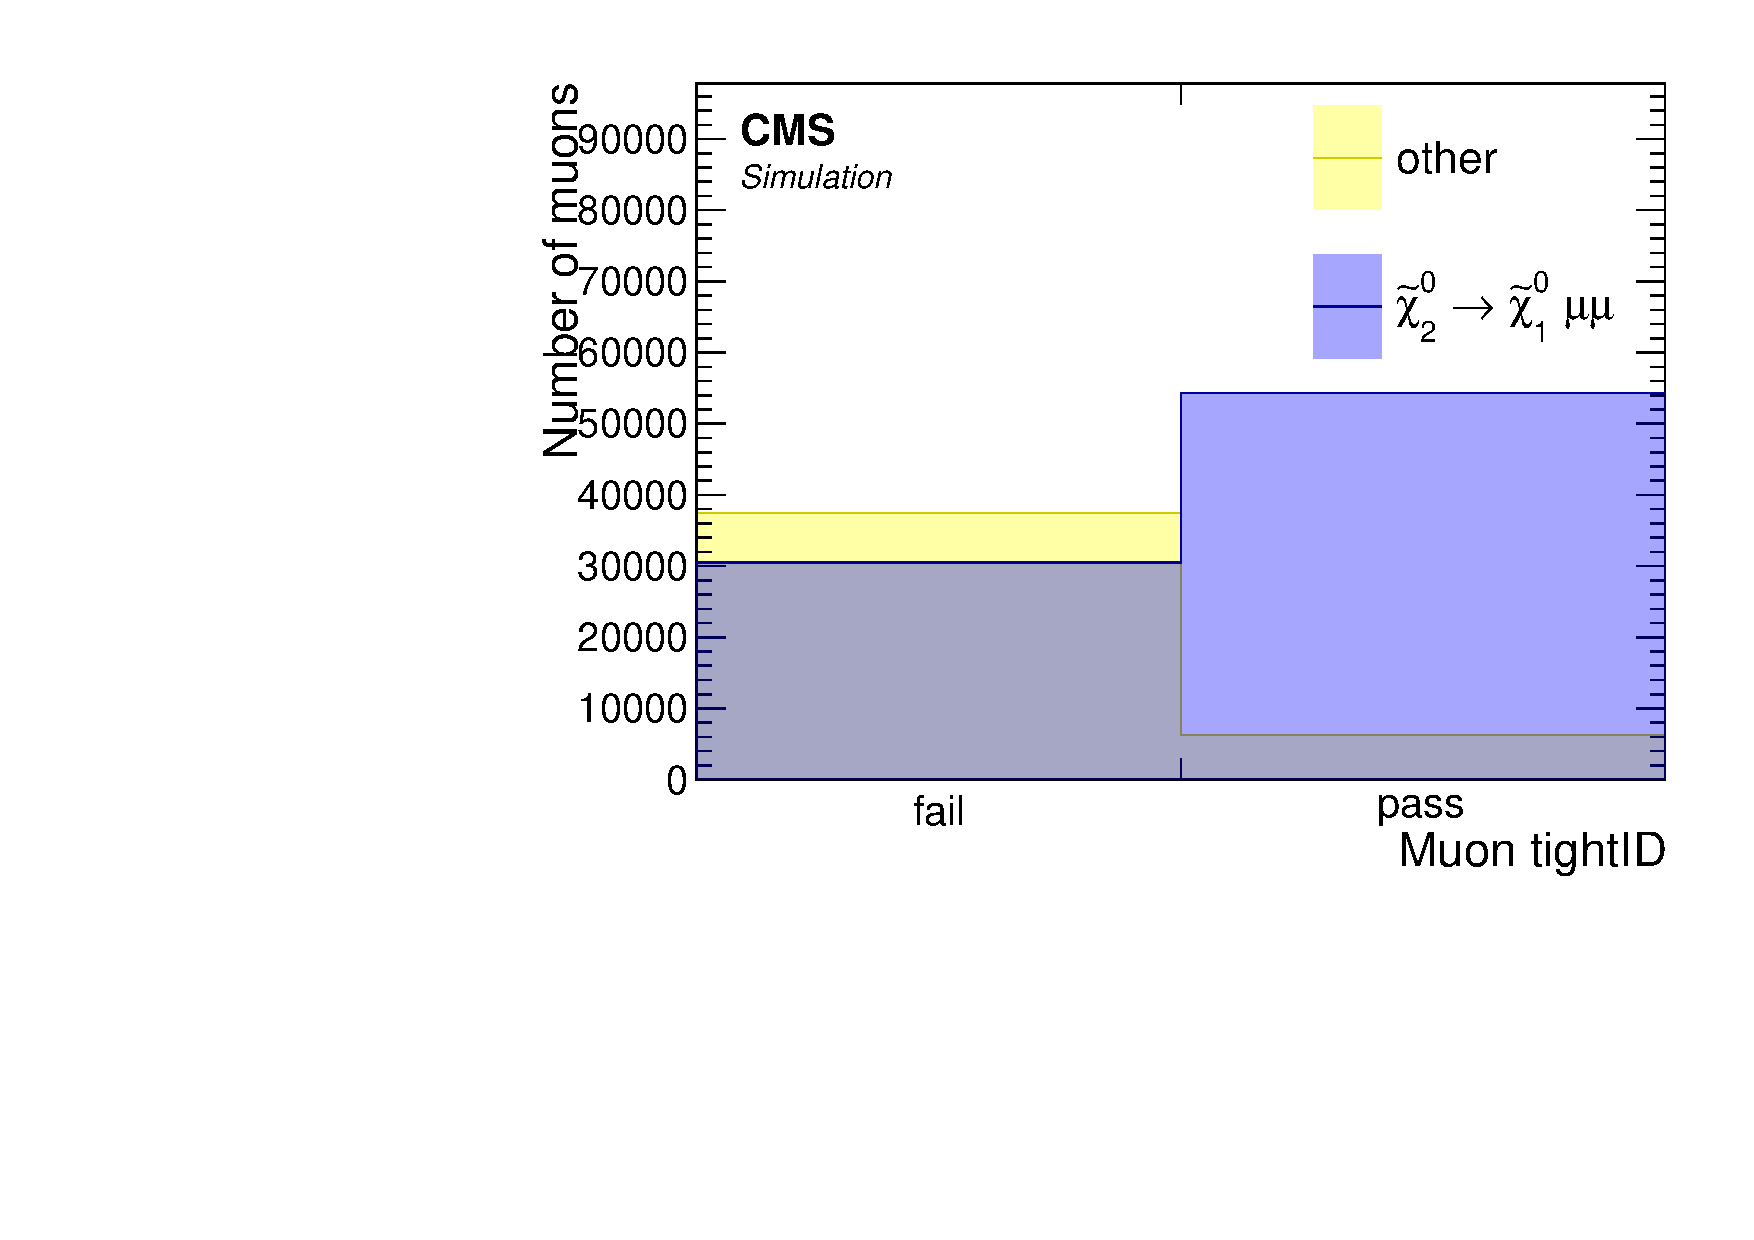
\includegraphics[width=0.32\linewidth]{plots/lepton_selection/lepton_selection_dm5p63/none_Muons_tight.pdf} \,
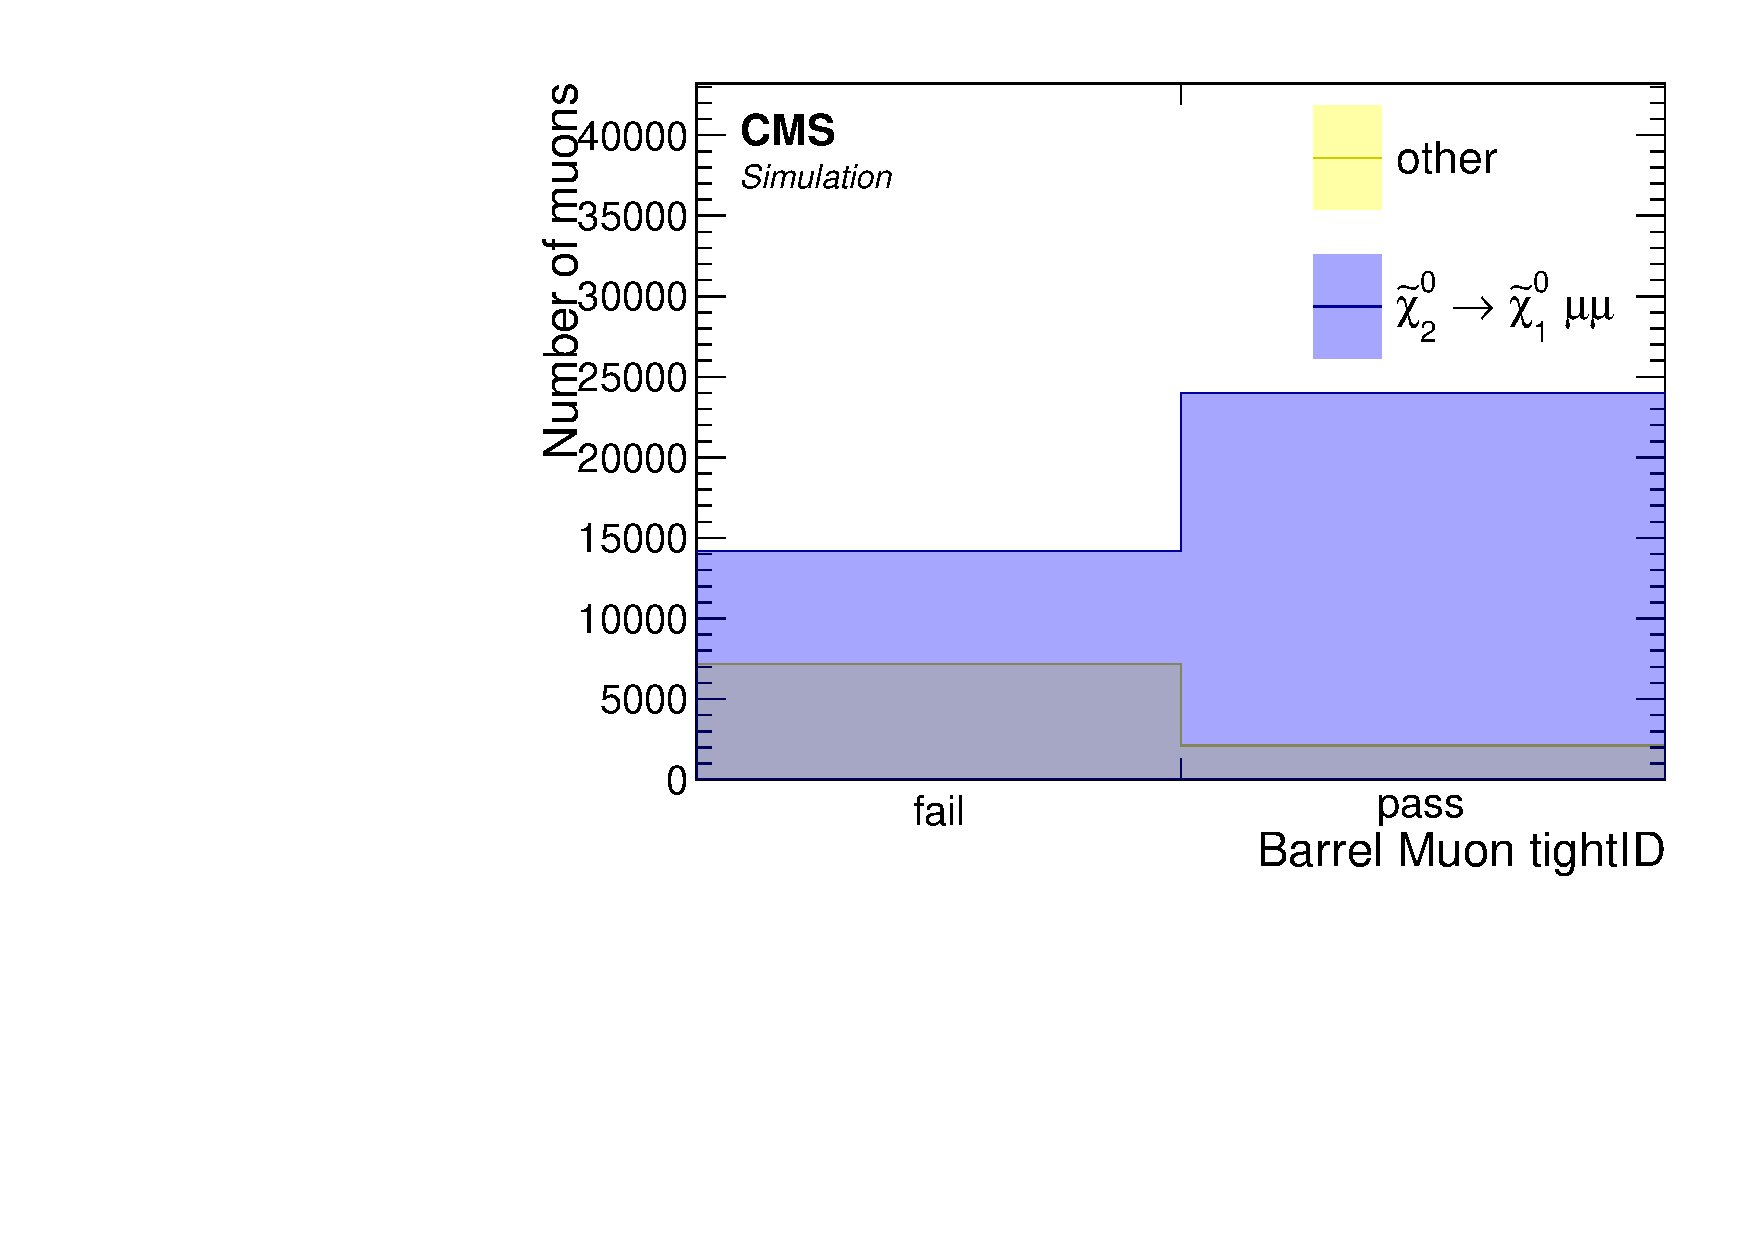
\includegraphics[width=0.32\linewidth]{plots/lepton_selection/lepton_selection_dm5p63/none_Muons_barrel_tight.pdf} \,
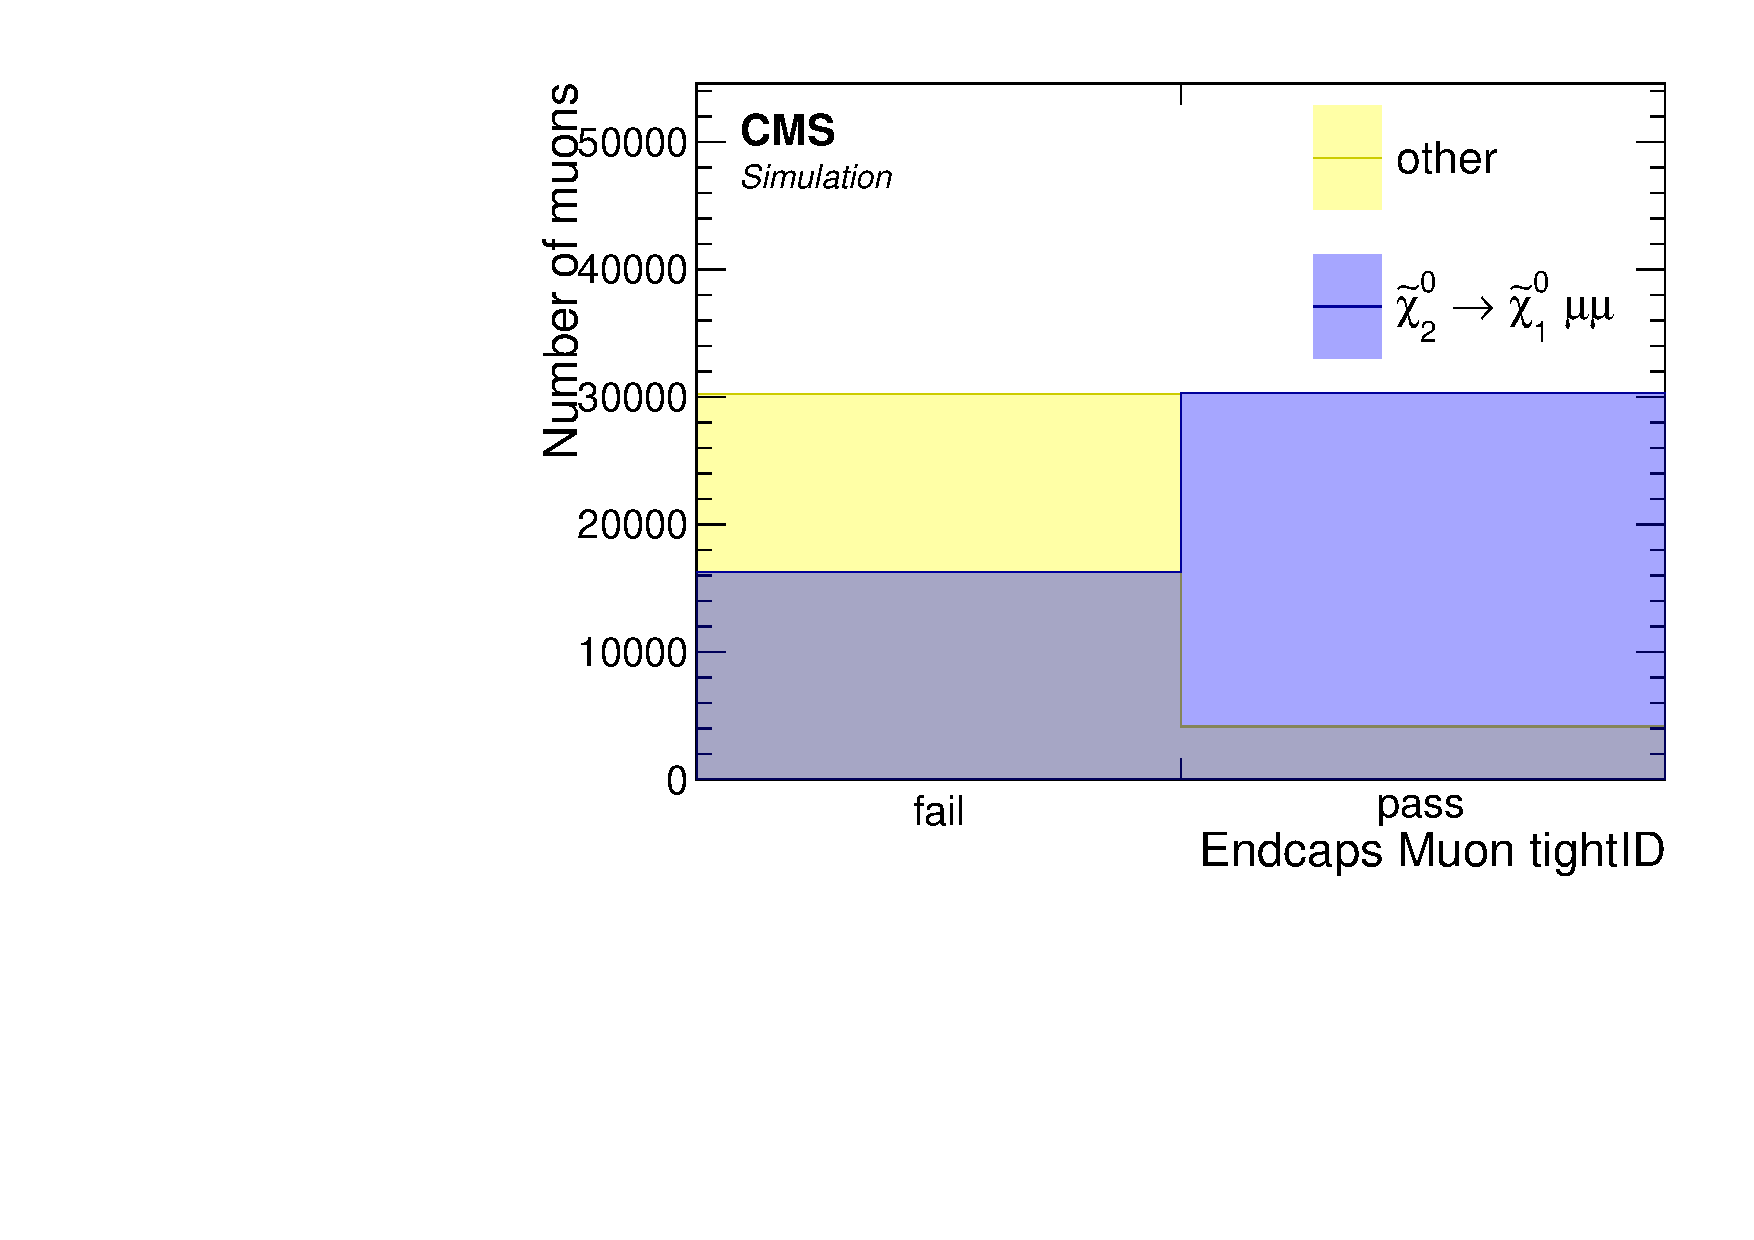
\includegraphics[width=0.32\linewidth]{plots/lepton_selection/lepton_selection_dm5p63/none_Muons_endcape_tight.pdf}   \\
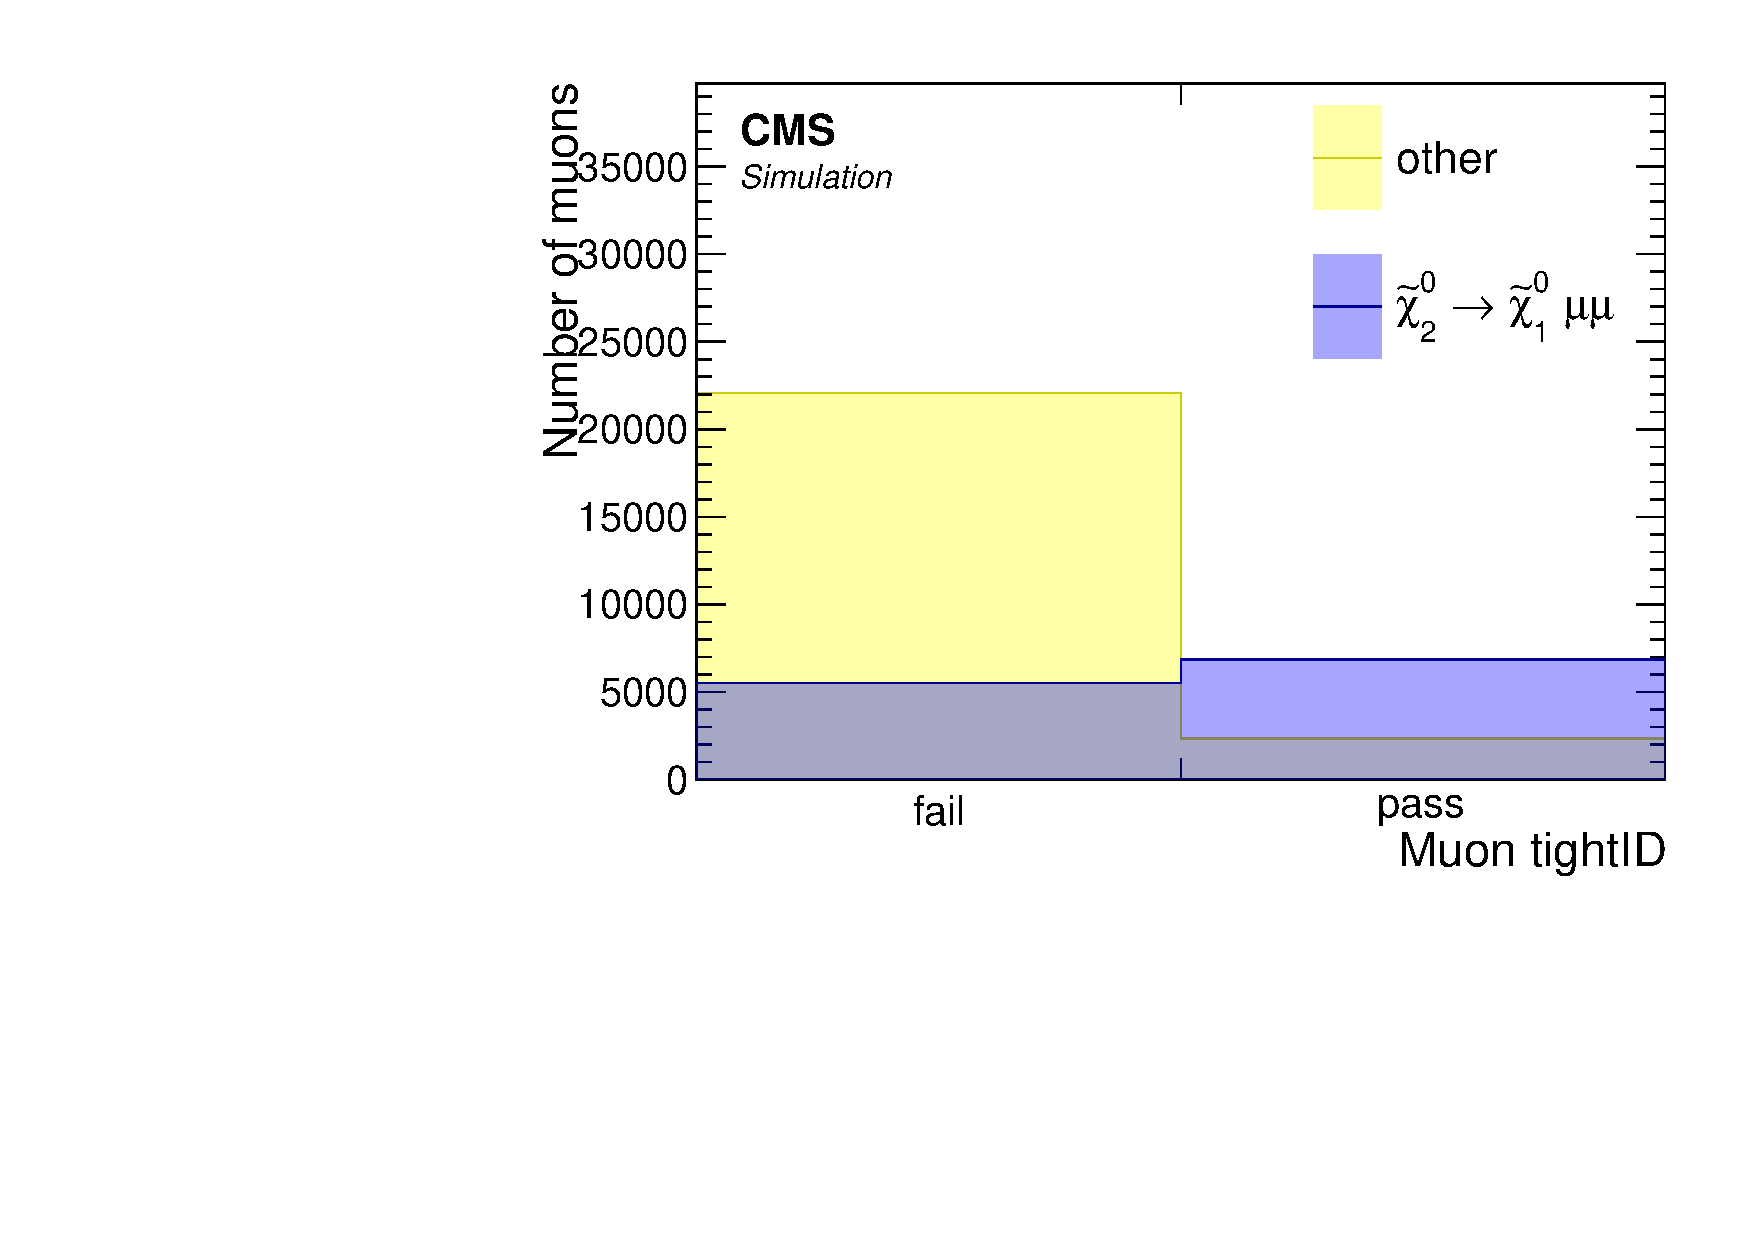
\includegraphics[width=0.32\linewidth]{plots/lepton_selection/lepton_selection_dm1p92/none_Muons_tight.pdf} \,
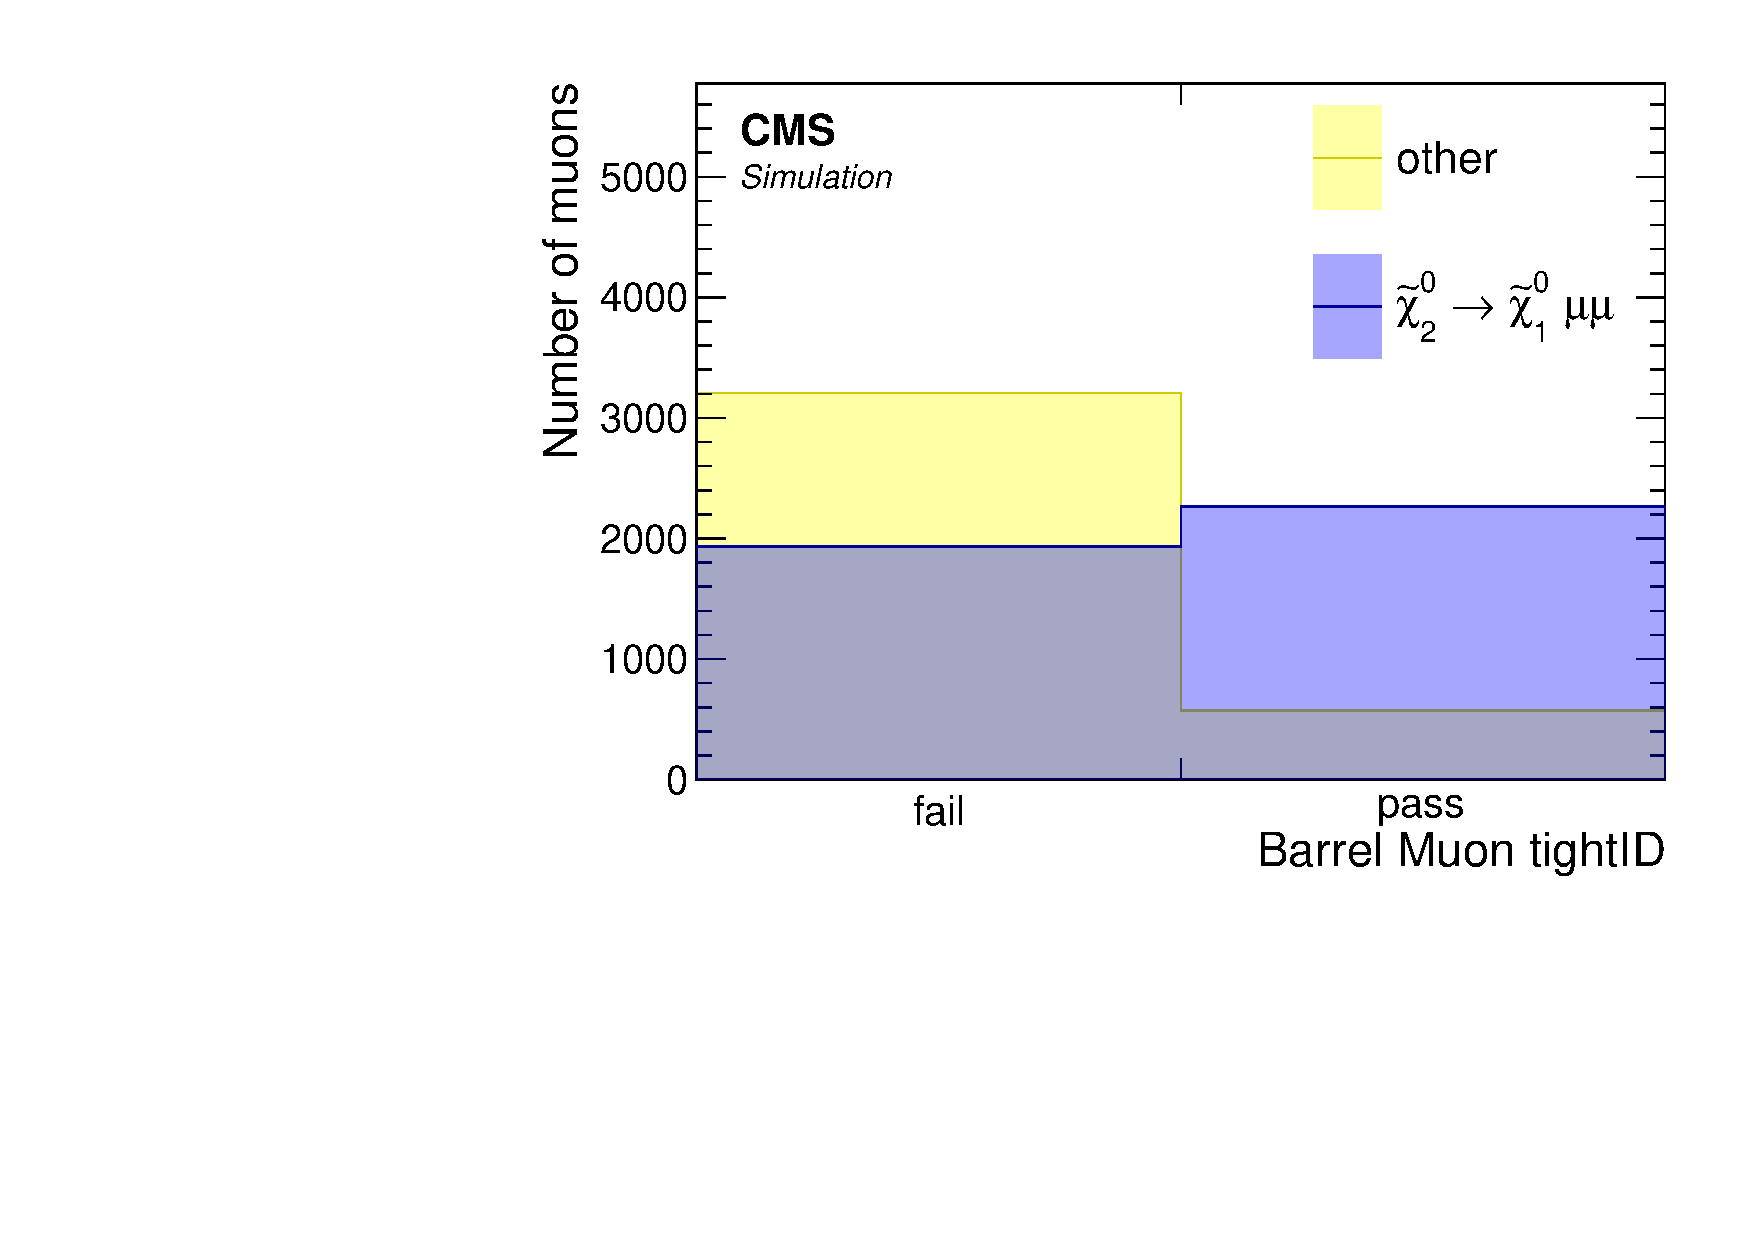
\includegraphics[width=0.32\linewidth]{plots/lepton_selection/lepton_selection_dm1p92/none_Muons_barrel_tight.pdf}  \,
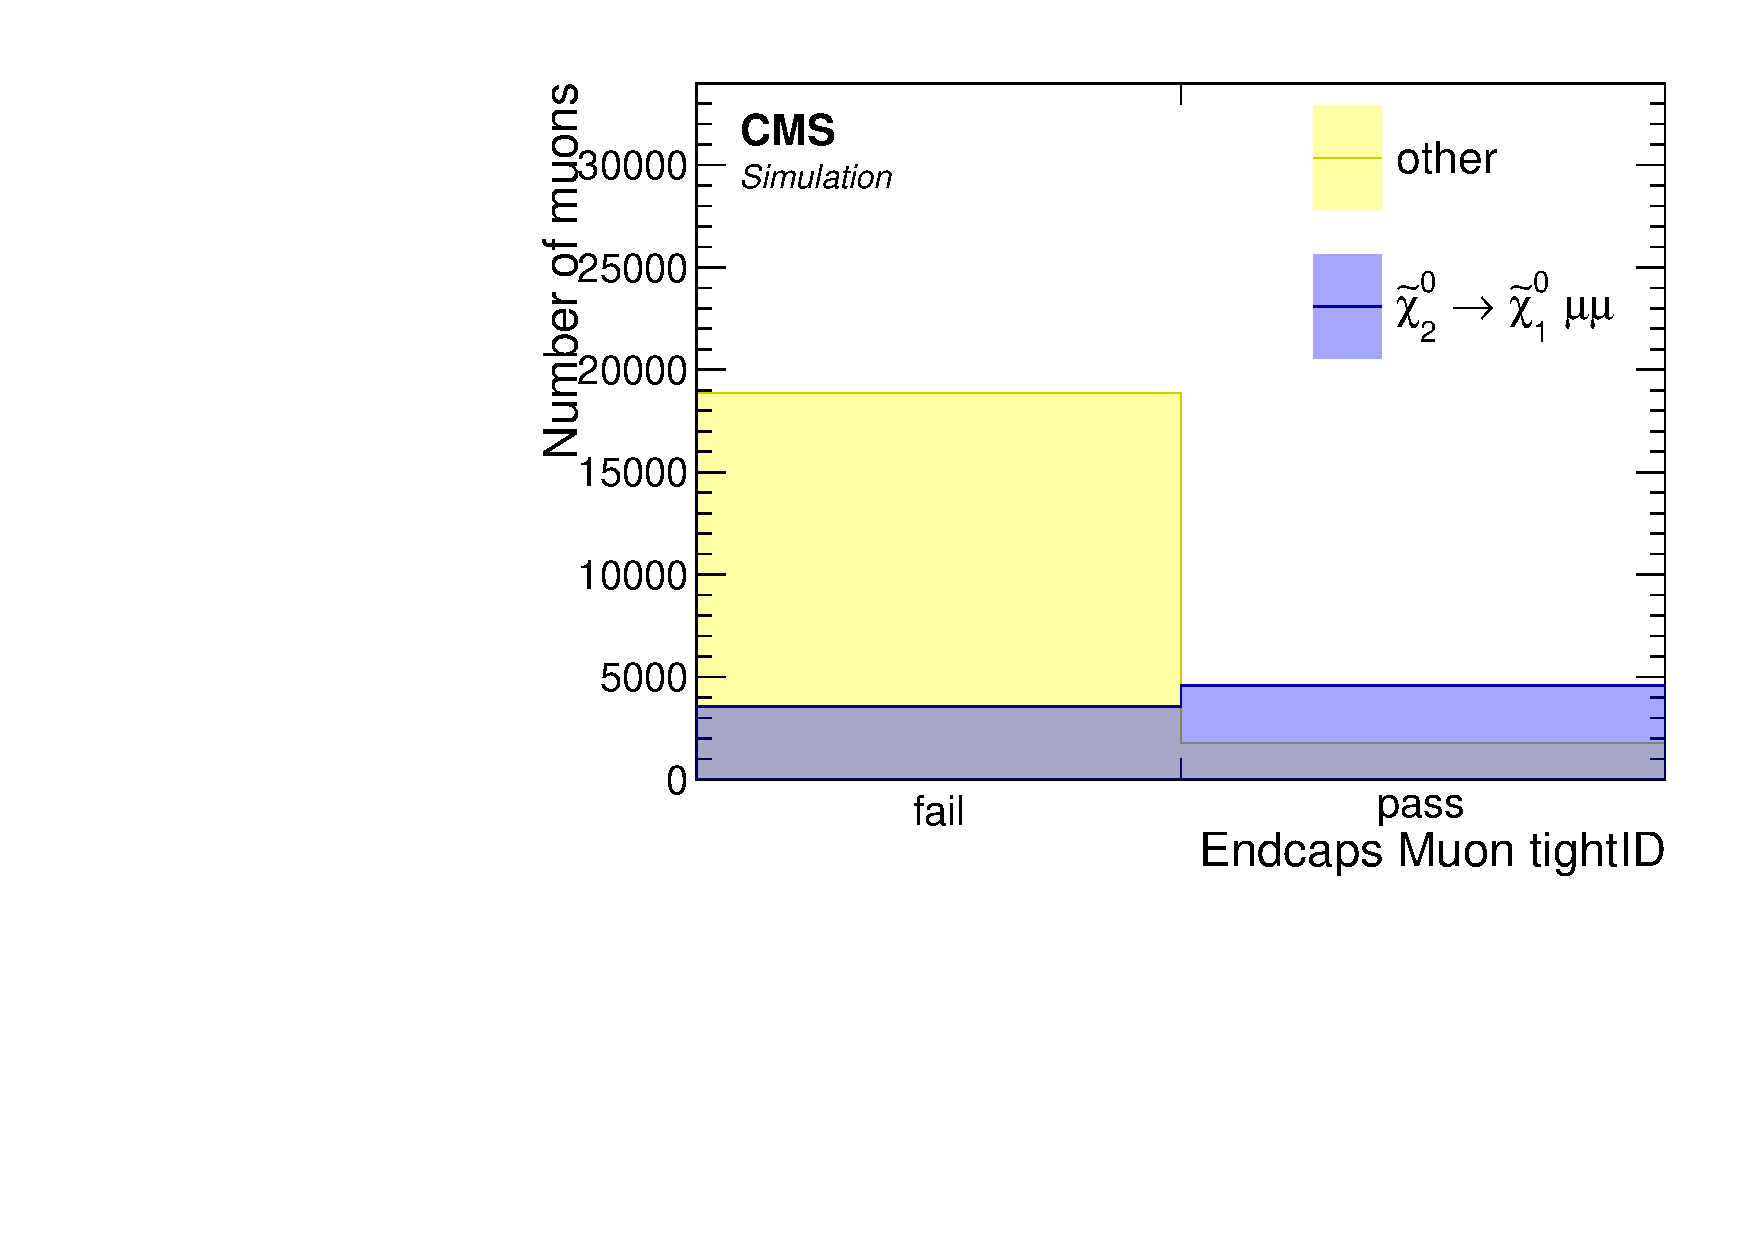
\includegraphics[width=0.32\linewidth]{plots/lepton_selection/lepton_selection_dm1p92/none_Muons_endcape_tight.pdf} \\
\caption[Tight ID \gls{wp} distribution of reconstructed muons]{Tight ID \gls{wp} distributions of reconstructed muons for $\dm=5.63\GeV$ (top) and $\dm=1.92\GeV$ (bottom) in the inclusive \pt case (left), barrel (middle) and endcaps (right). Cuts of $\DR(\jmath_1,\mu)>0.4$, $\pt>2\GeV$ and $\pt<15\GeV$ are applied.}
\label{fig:muons-selection-id-tight}
\end{figure}

The custom jet-isolation was designed to reject \gls{sm} background while retaining signal, as the effects of the custom jet-baed isolation, as described in Section~\ref{sec:isolation}, on signal muons is examined in this purity study. Figure~\ref{fig:muons-selection-isolation} shows that a small price is paid by requiring the isolation. However, as will be seen in Section~\ref{sec:isolation}, the sensitivity is increased by rejecting a significant portion of \gls{sm} background via the isolation criterion.

\begin{figure}[!htb]
\centering
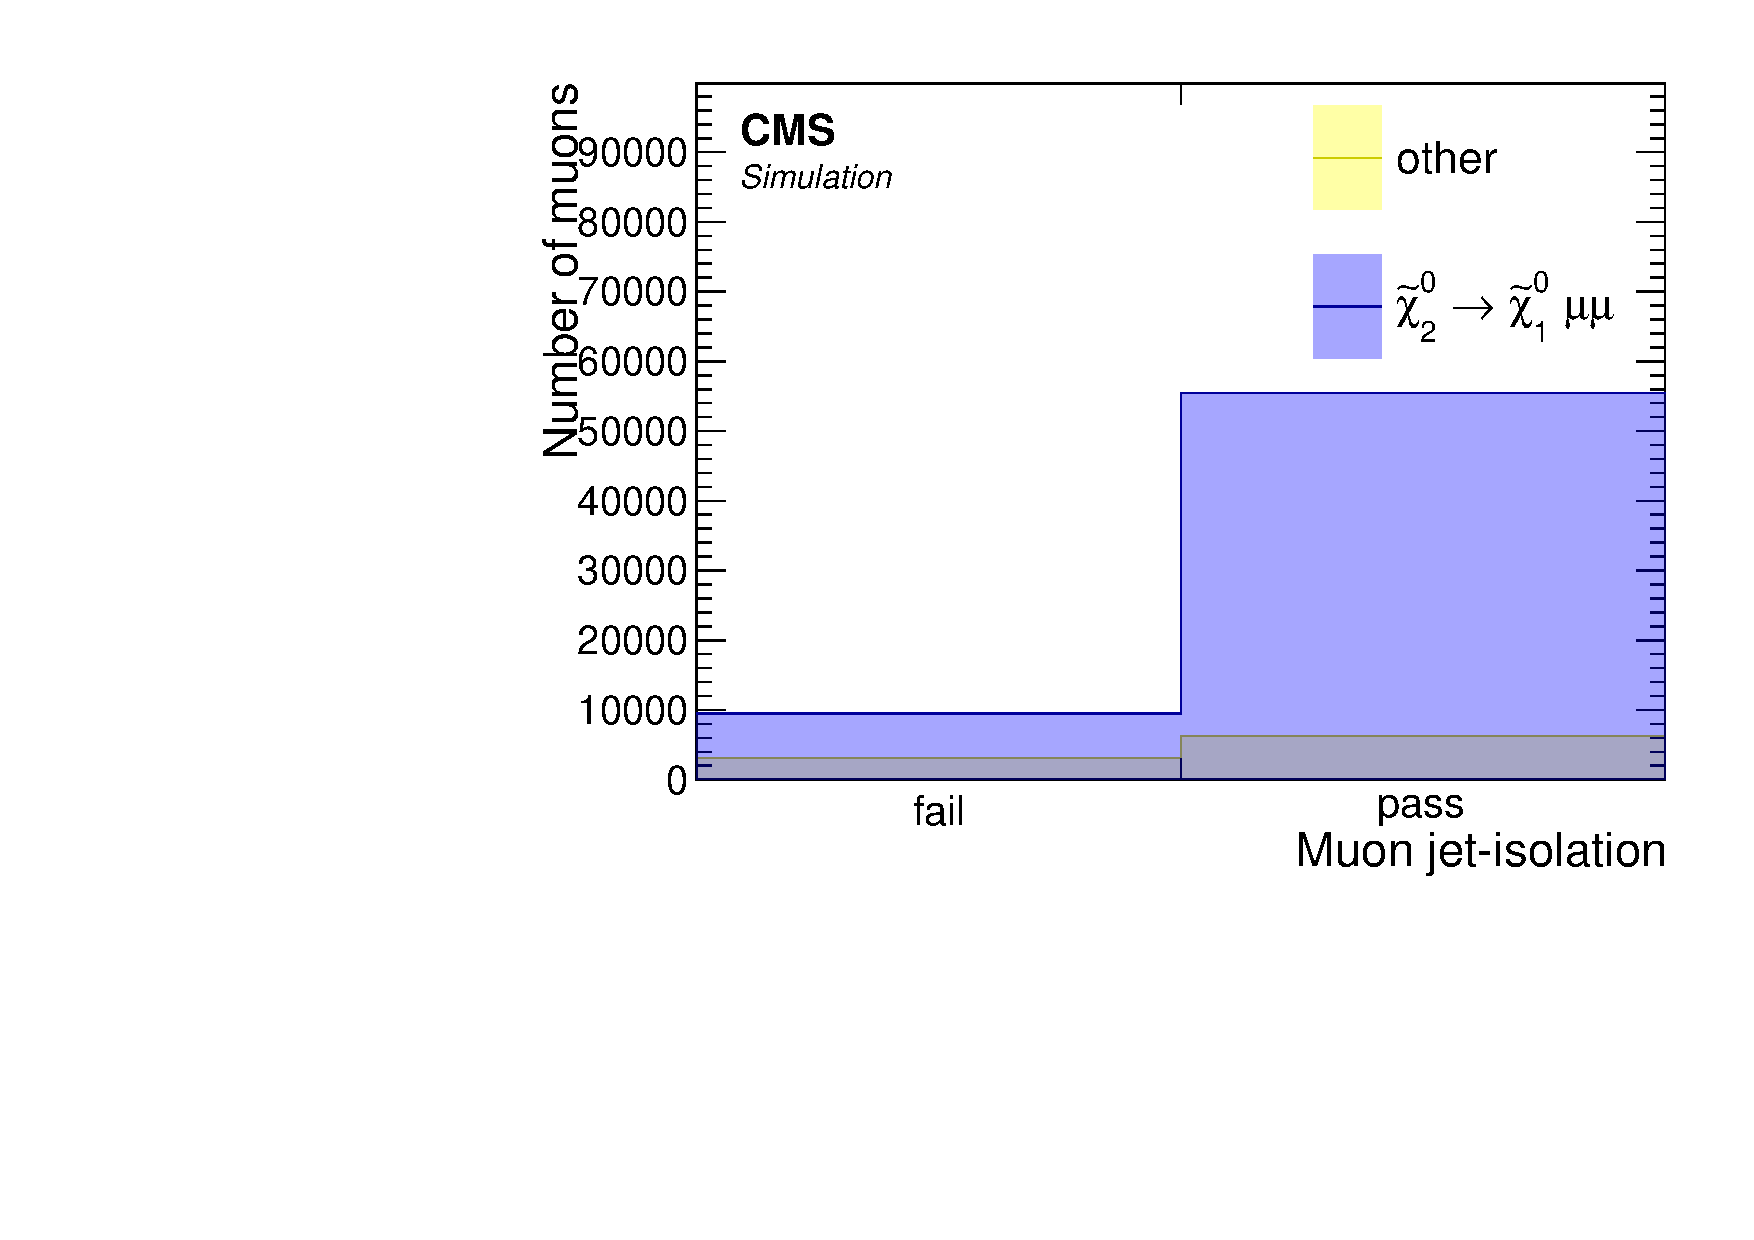
\includegraphics[width=0.32\linewidth]{plots/lepton_selection/lepton_selection_dm5p63/none_Muons_pt_jet_iso.pdf} \,
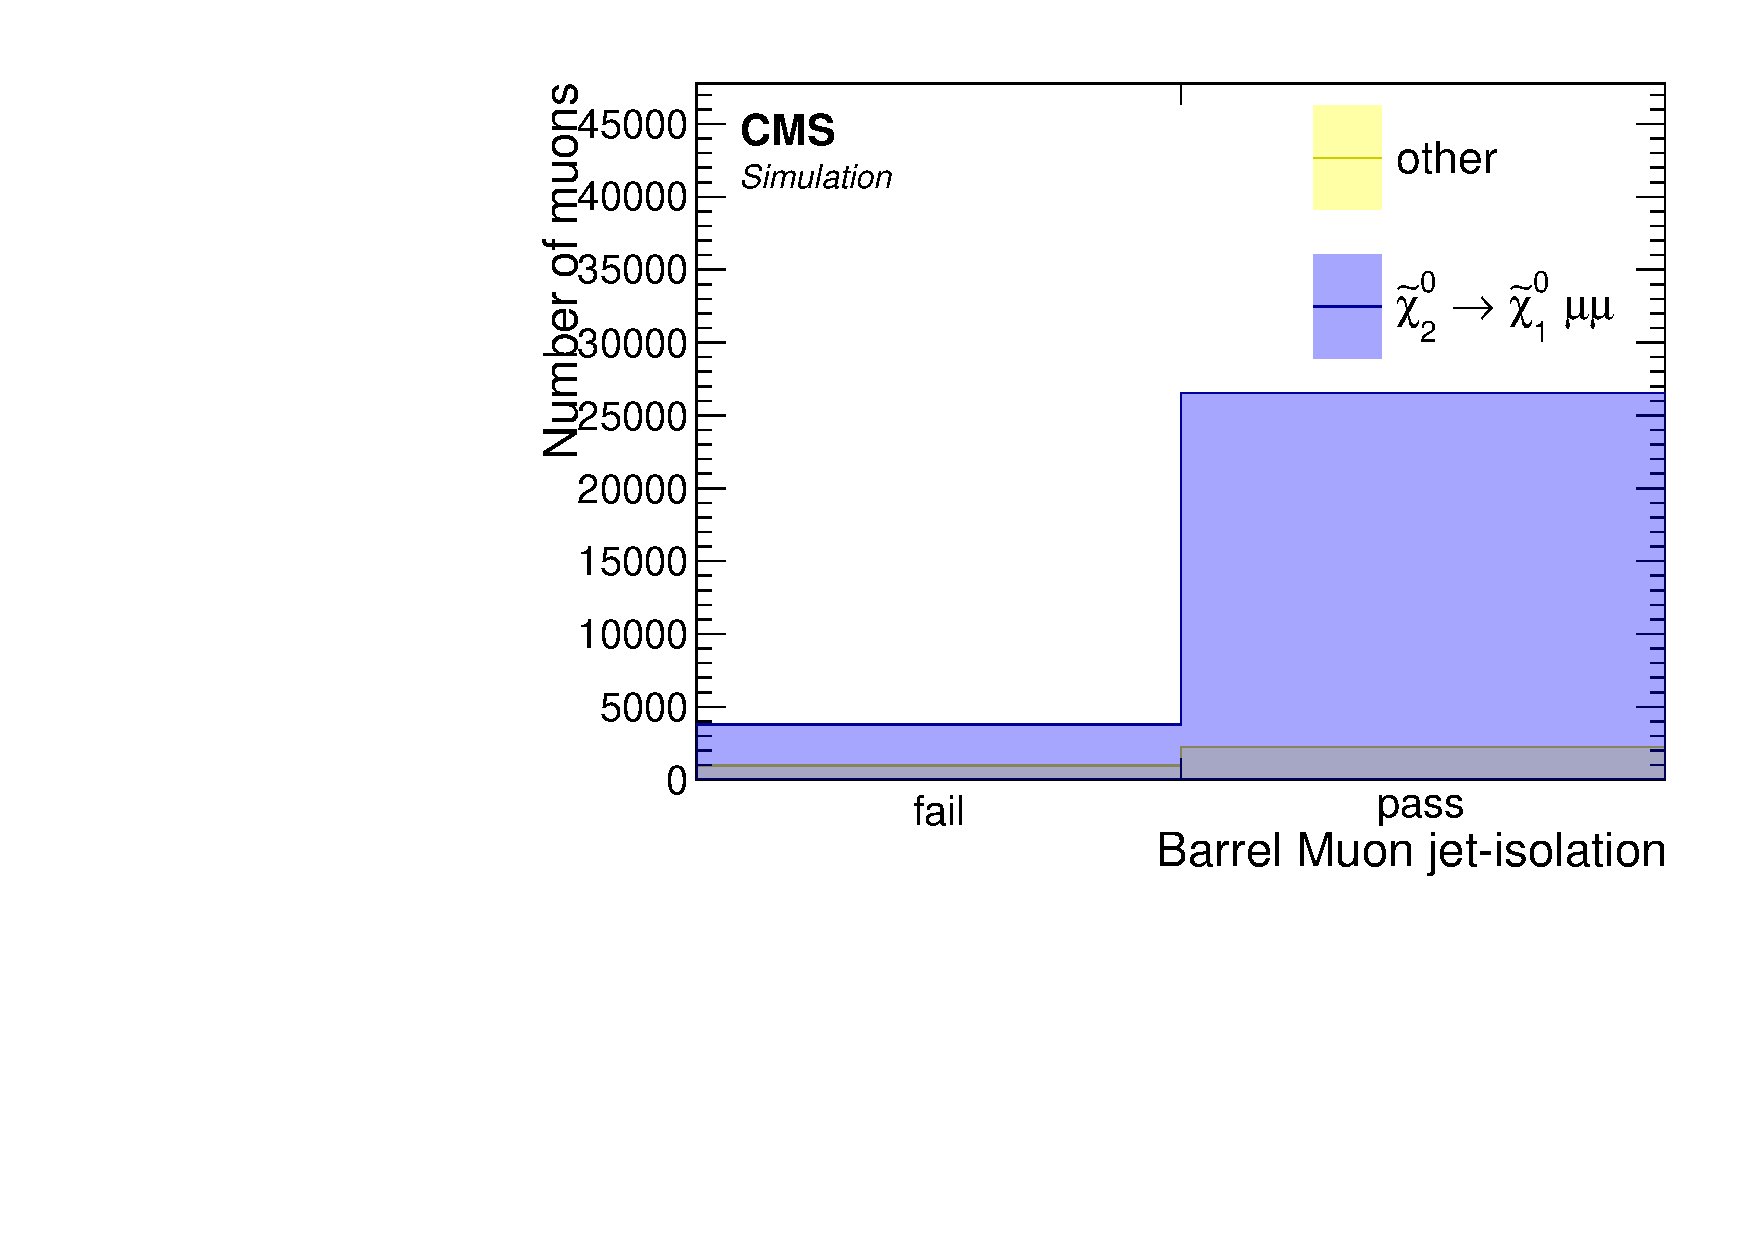
\includegraphics[width=0.32\linewidth]{plots/lepton_selection/lepton_selection_dm5p63/none_Muons_pt_barrel_jet_iso.pdf} \,
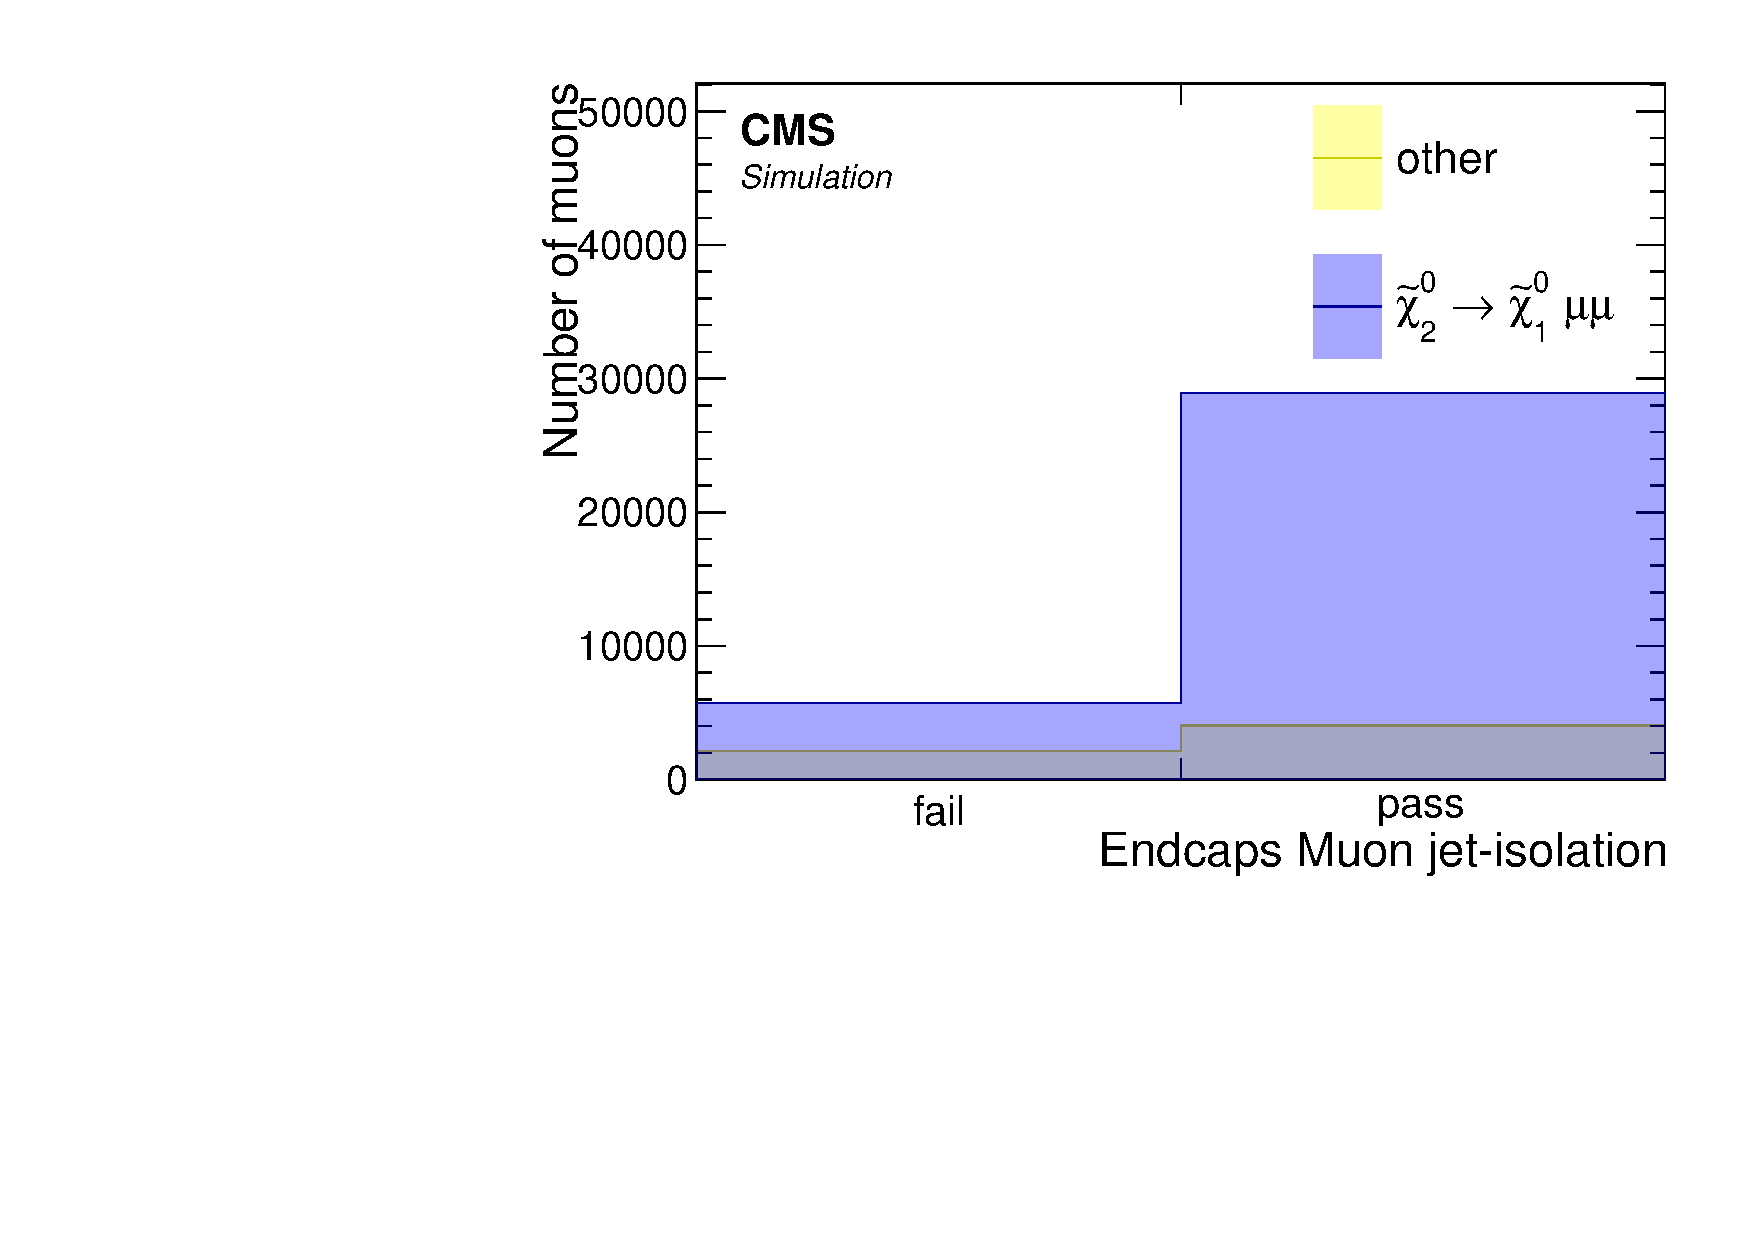
\includegraphics[width=0.32\linewidth]{plots/lepton_selection/lepton_selection_dm5p63/none_Muons_pt_endcape_jet_iso.pdf}   \\
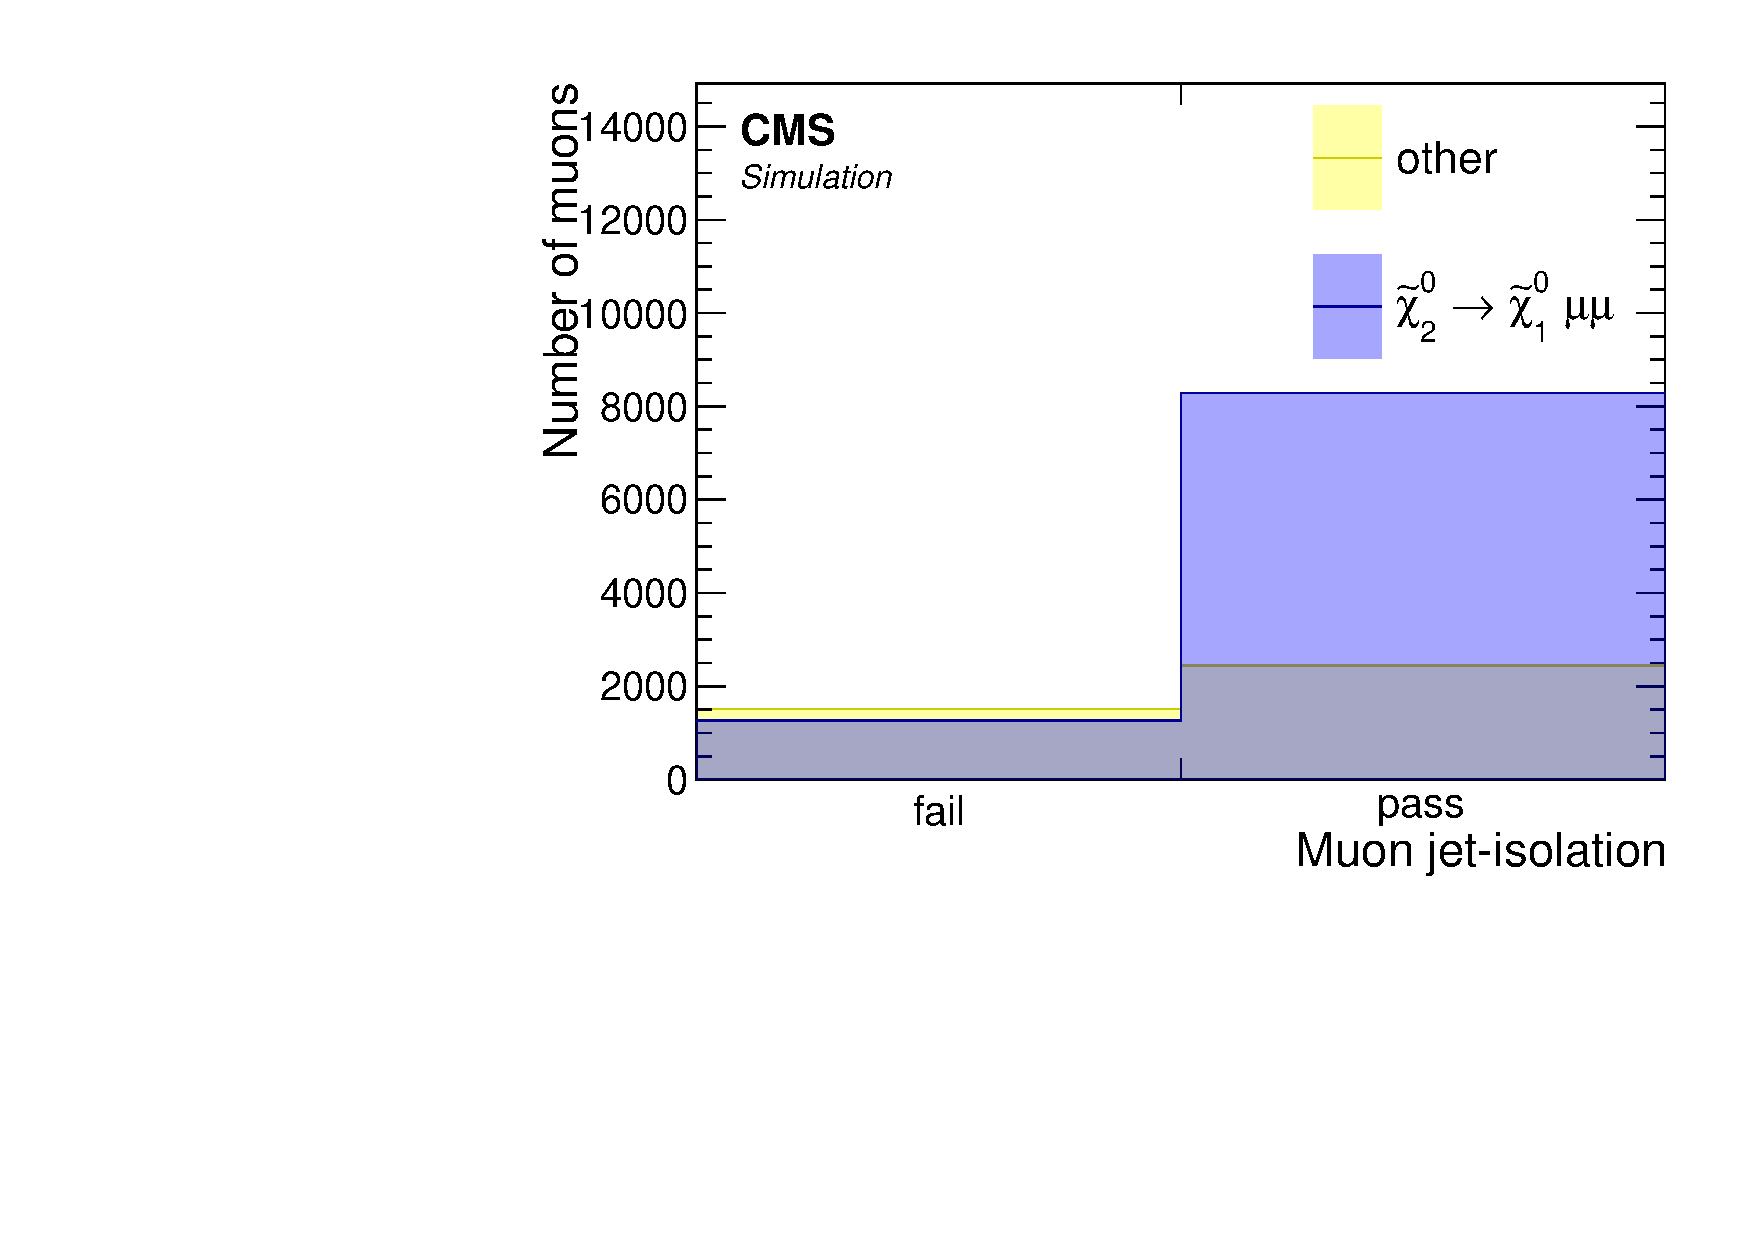
\includegraphics[width=0.32\linewidth]{plots/lepton_selection/lepton_selection_dm1p92/none_Muons_pt_jet_iso.pdf} \,
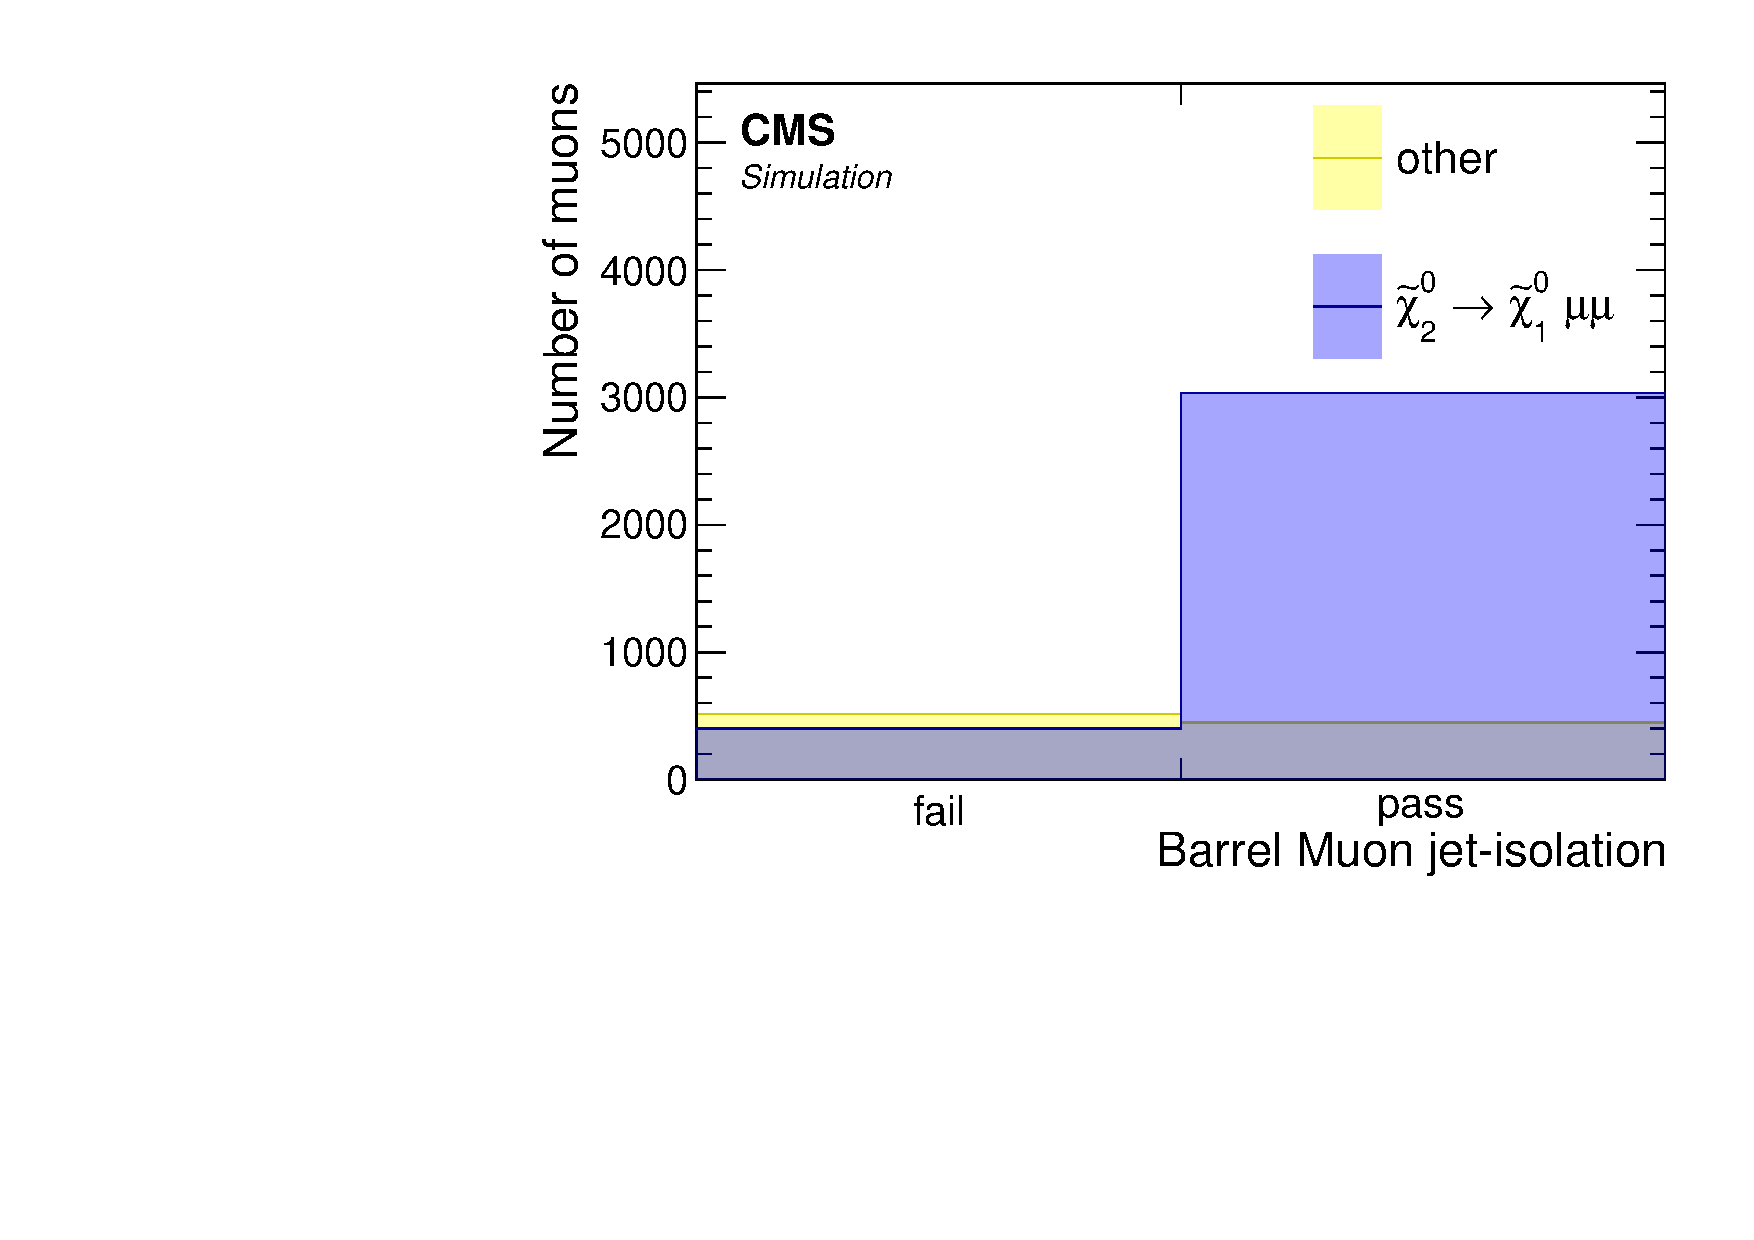
\includegraphics[width=0.32\linewidth]{plots/lepton_selection/lepton_selection_dm1p92/none_Muons_pt_barrel_jet_iso.pdf}  \,
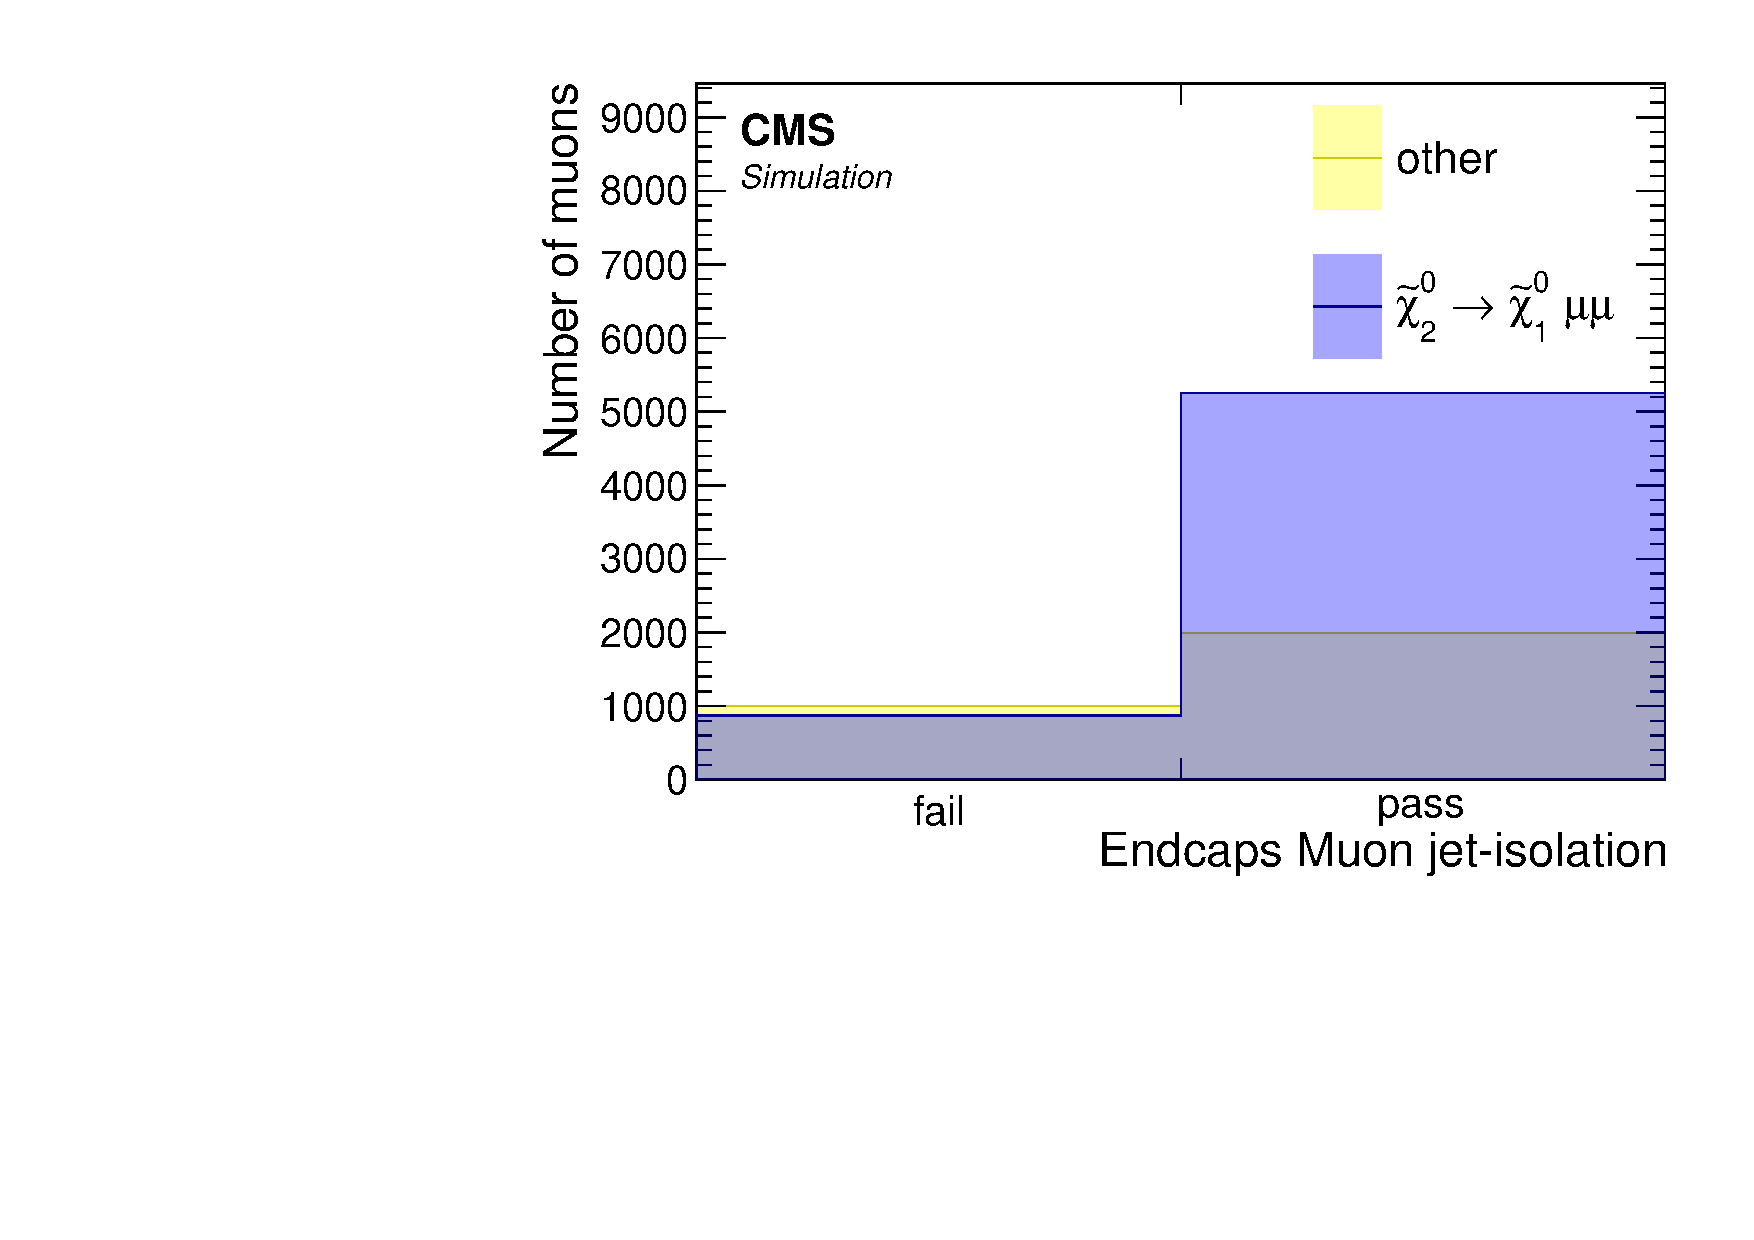
\includegraphics[width=0.32\linewidth]{plots/lepton_selection/lepton_selection_dm1p92/none_Muons_pt_endcape_jet_iso.pdf} \\
\caption[Distributions of the jet-based lepton isolation of reconstructed muons]{Distributions of the jet-based lepton isolation of reconstructed muons with Medium ID for $\dm=5.63\GeV$ (top) and $\dm=1.92\GeV$ (bottom) in the inclusive \pt case (left), barrel (middle) and endcaps (right). Cuts of $\DR(\jmath_1,\mu)>0.4$, $\pt>2\GeV$ and $\pt<15\GeV$ are applied.}
\label{fig:muons-selection-isolation}
\end{figure}

In summary, the following is the full set of selection criteria of the analysis muons:

\begin{itemize}
\item $2<\pt<15\GeV$;
\item $\abs{\eta} < 2.4$;
\item $\DR(\jmath_1,\mu)>0.4$;
\item Medium ID \gls{wp};
\item pass jet-isolation.
\end{itemize}


\begin{figure}[]
\centering
\includegraphics[width=0.32\linewidth]{plots/jpsi_muons_fit_bg_delta_r_single_electron/none_invMass_0_0.3_0_1.2.pdf} \,
\includegraphics[width=0.32\linewidth]{plots/jpsi_muons_fit_bg_delta_r_single_electron/none_invMass_0.3_0.5_0_1.2.pdf}  \,
\includegraphics[width=0.32\linewidth]{plots/jpsi_muons_fit_bg_delta_r_single_electron/none_invMass_0.5_1.5_0_1.2.pdf} \\
\includegraphics[width=0.32\linewidth]{plots/jpsi_muons_fit_bg_delta_r_single_electron/none_id_invMass_0_0.3_0_1.2.pdf} \,
\includegraphics[width=0.32\linewidth]{plots/jpsi_muons_fit_bg_delta_r_single_electron/none_id_invMass_0.3_0.5_0_1.2.pdf}  \,
\includegraphics[width=0.32\linewidth]{plots/jpsi_muons_fit_bg_delta_r_single_electron/none_id_invMass_0.5_1.5_0_1.2.pdf} \\
\caption[Barrel BG]{Barrel Muons BG}
\label{fig:tb-barrel-simulation}
\end{figure}

\begin{figure}[]
\centering
\includegraphics[width=0.32\linewidth]{plots/jpsi_muons_fit_bg_delta_r_single_electron/none_invMass_0_0.3_1.2_2.4.pdf} \,
\includegraphics[width=0.32\linewidth]{plots/jpsi_muons_fit_bg_delta_r_single_electron/none_invMass_0.3_0.5_1.2_2.4.pdf} \,
\includegraphics[width=0.32\linewidth]{plots/jpsi_muons_fit_bg_delta_r_single_electron/none_invMass_0.5_1.5_1.2_2.4.pdf} \\
\includegraphics[width=0.32\linewidth]{plots/jpsi_muons_fit_bg_delta_r_single_electron/none_id_invMass_0_0.3_1.2_2.4.pdf} \,
\includegraphics[width=0.32\linewidth]{plots/jpsi_muons_fit_bg_delta_r_single_electron/none_id_invMass_0.3_0.5_1.2_2.4.pdf} \,
\includegraphics[width=0.32\linewidth]{plots/jpsi_muons_fit_bg_delta_r_single_electron/none_id_invMass_0.5_1.5_1.2_2.4.pdf}  \\
\caption[Endcaps BG]{Endcaps Muons BG}
\label{fig:tb-endcaps-simulation}
\end{figure}

\begin{figure}[]
\centering
\includegraphics[width=0.32\linewidth]{plots/jpsi_muons_fit_data_delta_r_single_electron/none_invMass_0_0.3_0_1.2.pdf} \,
\includegraphics[width=0.32\linewidth]{plots/jpsi_muons_fit_data_delta_r_single_electron/none_invMass_0.3_0.5_0_1.2.pdf}  \,
\includegraphics[width=0.32\linewidth]{plots/jpsi_muons_fit_data_delta_r_single_electron/none_invMass_0.5_1.5_0_1.2.pdf} \\
\includegraphics[width=0.32\linewidth]{plots/jpsi_muons_fit_data_delta_r_single_electron/none_id_invMass_0_0.3_0_1.2.pdf} \,
\includegraphics[width=0.32\linewidth]{plots/jpsi_muons_fit_data_delta_r_single_electron/none_id_invMass_0.3_0.5_0_1.2.pdf}  \,
\includegraphics[width=0.32\linewidth]{plots/jpsi_muons_fit_data_delta_r_single_electron/none_id_invMass_0.5_1.5_0_1.2.pdf} \\
\caption[Barrel Data]{Barrel Muons Data}
\label{fig:tb-barrel-data}
\end{figure}

\begin{figure}[]
\centering
\includegraphics[width=0.32\linewidth]{plots/jpsi_muons_fit_data_delta_r_single_electron/none_invMass_0_0.3_1.2_2.4.pdf} \,
\includegraphics[width=0.32\linewidth]{plots/jpsi_muons_fit_data_delta_r_single_electron/none_invMass_0.3_0.5_1.2_2.4.pdf} \,
\includegraphics[width=0.32\linewidth]{plots/jpsi_muons_fit_data_delta_r_single_electron/none_invMass_0.5_1.5_1.2_2.4.pdf} \\
\includegraphics[width=0.32\linewidth]{plots/jpsi_muons_fit_data_delta_r_single_electron/none_id_invMass_0_0.3_1.2_2.4.pdf} \,
\includegraphics[width=0.32\linewidth]{plots/jpsi_muons_fit_data_delta_r_single_electron/none_id_invMass_0.3_0.5_1.2_2.4.pdf} \,
\includegraphics[width=0.32\linewidth]{plots/jpsi_muons_fit_data_delta_r_single_electron/none_id_invMass_0.5_1.5_1.2_2.4.pdf}  \\
\caption[Endcaps Data]{Endcaps Muons Data}
\label{fig:tb-endcaps-data}
\end{figure}

\clearpage

\subsection{Jets}
\label{subsec:jets}

Jets used in the analysis are reconstructed by clustering the \gls{pf} candidates using $\FASTJET$ with the anti-$\kt$ algorithm~\cite{Cacciari_2008_antikt} with a size parameter of 0.4. Tagging of $b$-jets is performed using the multivariate technique \DEEPCSV with a Medium \gls{wp}, also known as the \gls{csv} algorithm~\cite{BTV-16-002}. Jets are required to have a transverse momentum $\pt>30\GeV$ and $\abs{\eta}<2.4$.

\subsection{Missing transverse energy}
\label{subsec:met}

The importance of the missing transverse momentum (or energy) in this analysis has been discussed in Section~\ref{subsec:signal-met-mht}. Two standard measures of the momentum imbalance in the events are \VEtmiss (or \ptvecmiss by a different symbol) and \htvecmiss. \VEtmiss is defined as:
\begin{equation}
\VEtmiss = \ptvecmiss = -\sum_i \ptvec(i),
\end{equation}
where the summation is done on all particle flow candidates. Therefore, the missing transverse energy serves as a measure of particles that evade detection, such as weakly interacting neutral particles. Mismeasurements of visible particles and additional energy deposits from sources such as \gls{pu}, jet energy response and detector noise can affect this observable. To mitigate these effects, the correction process considers jets with \pt greater than $10\GeV$. Full details of the corrections can be found in~\cite{met_performance}.

An alternative measurement to the missing transverse momentum is \htvecmiss, which is sometimes referred to as \emph{missing hardronic activity}. Instead of considering all particle flow candidates in the sum, this measurement only takes into account jets with \pt greater than $30\GeV$ and $\abs{\eta}$ less than 5, and is defined as:
\begin{equation}
\htvecmiss = -\sum_i^{\mathrm{jets}} \ptvec(i).
\end{equation}

The observable \htvecmiss is favored over \VEtmiss in this analysis because the jet-based isolation, defined in Section~\ref{sec:isolation}, uses jets with \pt greater than $30\GeV$, while a sideband is defined using the range of $\pt\in [15,30]\GeV$ of jets, which is then used for the estimation of the jetty background in Section~\ref{sec:jetty-background-estimation}. Both observables, \VEtmiss and \htvecmiss, have equivalent scalar quantities, \MET and \mht respectively, which can be obtained by taking the magnitude of their vectorial counterpart.

\clearpage
\subsection{Tracks and multivariate selection}
\label{sec:track-bdt}

The leptons \ellell produced in the decay \neuttdecay tend to have very low transverse momentum \pt. The identification and reconstruction efficiency of the muons worsens with lower \pt. Therefore, the aim of the exclusive track category is to recover lost leptons that were not reconstructed or identified. The tracking efficiency for the \pt ranges used in this analysis is well above 99\%, allowing the recovery of some of the  tracks that correspond to the missing leptons.

To identify which track corresponds to the target lepton in a given signal event, \gls{bdt} classifiers are trained. Four separate \glspl{bdt} are trained, corresponding to each lepton flavor (muon or electron) and each phase of the tracker (Phase 0 for 2016, and Phase 1 for 2017-2018). All \glspl{bdt} use a common structure of 200 trees with a maximum depth of 3, and are trained with AdaBoost and GiniIndex separation using the TMVA package~\cite{tmva}. The package's default values are used for all other parameters. Tracks from a dedicated \FASTSIM signal simulations described in Section~\ref{sec:signal-simulation} are used for training. A broad range of simulated higgsino parameter $\mu$ (or the mass of \PSGcpmDo) is considered, but only the range of \dm that this analysis targets. For Phase 0, $\dmo$ is chosen from the range $[0.3,4.3]\GeV$ and $\mu$ from $[100-130]\GeV$, while for Phase 1, $\dmpm$ is chosen from $[0.3-4.6]\GeV$ and $\mu$ from $[100-500]\GeV$. Signal events are split into signal tracks and background tracks, with signal tracks originating from leptons from the decay \neuttdecay while background tracks do not match to the leptons. The samples for muons contain 9408 (10964) signal tracks and 99996 (151380) background tracks for Phase 0 (Phase 1). For electrons the samples contain 2364 (2288) signal tracks and 104065 (159713) background tracks for Phase 0 (Phase 1). The training samples is then tested with independent samples of equal size. 

Pre-selection is applied to all tracks in the collection obtained by the standard track reconstruction sequences. This pre-selection ensures that only properly-reconstructed, isolated, and prompt tracks are considered. The selected tracks must also have trajectories passing through the region near the primary vertex (PV). The full set of track pre-selection criteria are
\begin{itemize}
\item $ \pt > 1.9 \GeV$;
\item $ \abs{\eta} < 2.4$;
\item track $\text{iso}_\text{rel}  < 0.1$, using \DR(track, other tracks) $< 0.3$;
\item $d_{xy}(\text{track, PV}) < 0.02\, \cm$ w.r.t the PV;
\item $d_z(\text{track, PV}) < 0.02\, \cm$ w.r.t the PV
\item no match to an electron or muon within a cone of size 0.01.
\end{itemize}
For the training, a set of 10 variables, listed in Table~\ref{tab:track-bdt-variables} in decreasing order of their importance ranking of the BDT training (in the muon case of Phase 0) is used.

\begin{table}[!htb]
	\centering
	\label{tab:track-bdt-variables}
		\caption{Input variables to the in-signal track selecting classifier.}
		%\vspace{1mm}
			\begin{tabular}{cll} \hline
			Rank & Variable & Description \\ \hline
			1 & $\DR\left(t, \ell\right)$ & $t$ is the track and $\ell$ the lepton\\
			2 & $\abs{\Delta \eta \left(t, \ell\right) }$ & \\
			3 & $\pt(\ell)$ & \\
			
			4 & $\abs{\Delta\phi\left(t, \htvecmiss \right)}$ & \\
			5 & $\abs{\Delta\eta\left(t, j_1 \right)}$ & $j_1$ is the leading \pt jet\\
			6 & $\abs{\Delta\phi\left(t, \ell \right)}$ & \\
			7 & $\abs{\eta\left(t\right)}$ & \\
			8 & $\abs{\eta\left(\ell\right)}$ & \\
			9 & $\DR\left(\ell, j_1\right)$ & \\
			10 & $\mlt$ & invariant mass \\ 
			\hline
			\end{tabular}
\end{table}

Figure~\ref{fig:muon-track-bdt-inputs} shows the distribution of input variables, where signal tracks are shown in blue and background tracks in red.

\begin{figure}[!htb]
\centering
\includegraphics[width=0.32\linewidth]{plots/track_bdt_inputs_muons/none_deltaRLL.pdf} \,
\includegraphics[width=0.32\linewidth]{plots/track_bdt_inputs_muons/none_deltaEtaLL.pdf} \,
\includegraphics[width=0.32\linewidth]{plots/track_bdt_inputs_muons/none_lepton.Pt__.pdf} \\

\includegraphics[width=0.32\linewidth]{plots/track_bdt_inputs_muons/none_deltaPhiMht.pdf} \,
\includegraphics[width=0.32\linewidth]{plots/track_bdt_inputs_muons/none_deltaEtaLJ.pdf} \,
\includegraphics[width=0.32\linewidth]{plots/track_bdt_inputs_muons/none_abs_deltaPhiLL_.pdf}  \\

\includegraphics[width=0.32\linewidth]{plots/track_bdt_inputs_muons/none_abs_track.Eta___.pdf} \,
\includegraphics[width=0.32\linewidth]{plots/track_bdt_inputs_muons/none_abs_lepton.Eta___.pdf} \,
\includegraphics[width=0.32\linewidth]{plots/track_bdt_inputs_muons/none_deltaRLJ.pdf}  \\


\includegraphics[width=0.32\linewidth]{plots/track_bdt_inputs_muons/none_invMass.pdf}  \\


\caption[Muon track BDT training inputs]{Distibutions of the inputs to the track BDT in the muon exclusive track category. Fake category refers to tracks not originating from target leptons.}
\label{fig:muon-track-bdt-inputs}
\end{figure}

The classifier output score for the 4 \glspl{bdt} is displayed in Figure~\ref{fig:track-bdt-output}, where the test distributions are superimposed on the training sample. No obvious over-training is observed. The ROC curves are plotted in Figure~\ref{fig:track-bdt-roc}, where the red points indicate the efficiency of the signal and background tracks of the minimum BDT cut, which is taken to be 0.0. Good separation between signal tracks and fake tracks is obtained, as evidenced by the relatively high signal efficiency of over 90\% (86\%) for muons (electrons) and background rejection of around 86\% (76\%) for muons (electrons).

\begin{figure}[!htb]
\centering
\includegraphics[width=0.48\linewidth]{plots/track_bdt/overtraining_Tracks_Muons_Phase_0.pdf} \,
\includegraphics[width=0.48\linewidth]{plots/track_bdt/overtraining_Tracks_Muons_Phase_1.pdf}  \\
\includegraphics[width=0.48\linewidth]{plots/track_bdt/overtraining_Tracks_Electrons_Phase_0.pdf} \,
\includegraphics[width=0.48\linewidth]{plots/track_bdt/overtraining_Tracks_Electrons_Phase_1.pdf} \\
\caption[Track BDT output plots]{Track BDT output plots for muons (top) and electrons (bottom) in Phase 0 (left) and Phase 1 (right). Blue shows signal tracks, while red are fake tracks. Test sample overlay on top of training sample.}
\label{fig:track-bdt-output}
\end{figure}

\begin{figure}[!htb]
\centering
\includegraphics[width=0.48\linewidth]{plots/track_bdt/roc_Tracks_Muons_Phase_0.pdf} \,
\includegraphics[width=0.48\linewidth]{plots/track_bdt/roc_Tracks_Muons_Phase_1.pdf}  \\
\includegraphics[width=0.48\linewidth]{plots/track_bdt/roc_Tracks_Electrons_Phase_0.pdf} \,
\includegraphics[width=0.48\linewidth]{plots/track_bdt/roc_Tracks_Electrons_Phase_1.pdf} \\
\caption[Track BDT ROC curves]{Track BDT ROC curves for muons (top) and electrons (bottom) in Phase 0 (left) and Phase 1 (right). The minimum threshold on the classifier score is indicated by the red dot.}
\label{fig:track-bdt-roc}
\end{figure}

The track with the maximum \gls{bdt} score is selected as the signal candidate track. Only events with a track with a score greater than 0.0, corresponding to the red dot in the ROC curves shown in Figure~\ref{fig:track-bdt-roc}, are considered.

\clearpage
\subsection{Isolation}
\label{sec:isolation}

The leptons produced from the neutralino decay \neuttdecay are typically isolated, with very little hadronic activity n their vicinity. This is because the only jets in the event come from initial state radiation, which boosts the produced electroweakinos in the opposite direction. Therefore, the leptons originating from those electroweakinos will not propagate collinear to these jets. The characteristic signal event topology can be exploited to distinguish signal events from background originating from \gls{sm} processes. At \gls{cms}, various standard isolation criteria are used. The three most widely used isolation criteria are track relative isolation~\cite{muon-pog-recommendations}, \gls{pf} relative isolation ($\mathrm{RelIso}$), which was first described in~\cite{Chatrchyan_2011}, and a modified version referred to as relative mini-isolation ($\mathrm{miniRelIso}$), described in~\cite{Rehermann_2011}.

Track relative isolation is defined as the \pt sum of all tracks around a given track (or lepton) within an angular separation $\DR$ of 0.3:

\begin{equation}
\text{Track relative isolation}_\ell = \frac{ \sum_{\substack{\text{tracks from PV}\\ \text{in } \DR<0.3}}\pt}{ \pt(\ell) }.
\end{equation}

Since only tracks are summed, only charged particles are taken into account. Another widely used isolation is the relative isolation which uses a cone size of 0.4 and defined as:
\begin{equation}
\text{RelIso}_\ell = \frac{ \sum_{\substack{\text{charged}\\\text{hadrons}\\\text{from PV}}}\pt + \max\left(0, \sum_{\substack{\text{neutral}\\\text{hadrons}}}\et + \sum_{\text{photons}}\et - 0.5\cdot \sum_{\substack{\text{charged}\\\text{hadrons}\\\text{from PU}}}\pt \right) }{ \pt(\ell) }.
\end{equation}
The last term in the definition is a correction for \gls{pu} effects. A lepton is considered to be isolated if its RelIso value is small. A variant of the relative isolation is the so-called mini relative isolation (miniRelIso), which differs from the standard relative isolation in that its cone size is dependent on the \pt of the lepton, as follows:
\begin{equation}
\DR = 
\begin{dcases}
0.2 & \pt(\ell)\leq 50\GeV \\
\frac{10\GeV}{\pt(\ell)} & \pt(\ell) \in (50\GeV , 200\GeV) \\
0.05 & \pt(\ell)\geq 200\GeV
\end{dcases}.
\end{equation}
The variable size cone allows for the recovery of efficiency when leptons are produced in the decay chain of a boosted object. In such cases, when the boost is large, the lepton is likely to overlap with another lepton produced at a common decay vertex, failing a standard isolation cut. The parameters are tuned to, and thus well-suited to, leptons from the decay of on-shell \PW and \PZ bosons, but are not suitable for low-mass resonances. 

The drawback of standard isolation criteria in the case of this analysis, is that the two leptons can compromise each other's isolation. As shown in Section~\ref{sec:lepton-dr}, access to low \dm model-points requires including the $\DR<0.3$ phasespace region. Requiring any of the standard isolation criteria will thus result in rejecting valuable signal events. An alternative isolation criterion is proposed to help retain some of the desired phasespace while rejecting the majority of the standard model background. This alternative isolation proves to be useful not only for optimally selecting leptons, but also for defining a sideband control region needed for the jetty background estimation, as described in Section~\ref{sec:jetty-background-estimation}. The steps to construct the alternative \emph{jet-based isolation} are described algorithmically below.
\begin{enumerate}
\item Subtract the vector 4-momenta of candidate leptons of a given flavor from any reconstructed jet $\DR$ smaller than 0.4
\item The lepton is said to pass isolation if it does not lie within $\DR<r$ of any \emph{lepton-corrected} jet with $\pt > p$. 
\item Lepton is said to fail isolation for background estimation if it fails \emph{jet-based isolation}, and the nearest uncorrected jet has $15<\pt<30\GeV$ (see~\ref{sec:jetty-background-estimation} for use of such lepton)
\end{enumerate}
The main idea behind defining jet-isolation is to reject leptons with hadronic activity around them while not losing a lepton that is close to another lepton of the same flavor. The process described introduces two free parameters: the \pt threshold of the lepton-corrected jets that cause a lepton's isolation to fail ($p$), and the cone size ($r$), which determines how close a corrected jet is allowed to be to a lepton. To choose the thresholds for these parameters, a scan is performed ranging over $p\in [0,20]\GeV$ and $r\in[0.4,0.6]$. For each step in the scan, the full analysis is performed, including the background estimation procedure which makes use of the jet-based isolation, and various performance criteria are extracted to inform the choice of optimum $r$ and $p$.  The criteria of interest include signal efficiency (which should be high), background efficiency (which should be low), signal contamination in control-regions (ideally low), jetty-background transfer factor (ideally less than 1), and lastly, the significance, which is computed taking into account transfer factor error on the background (which should be maximized). The scan is carried out for muons using 2016 \gls{mc} and data, and the results are shown in Tables~\ref{tab:iso-scan-signal-efficiency}-~\ref{tab:iso-scan-significance}.

\begin{table}[!htb]
	\centering
	\label{tab:iso-scan-signal-efficiency}
		\caption{Signal efficiency for the jet-based isolation scan for the dimuon channel, based on 2016 MC samples.}
		%\vspace{1mm}
			\begin{tabular}{cc|ccccc}
    			&\multicolumn{1}{c}{} & \multicolumn{5}{c}{$r$} \\
    && 0.4 & 0.45 & 0.5 & 0.55 & 0.6 \\
    \cline{2-7}
    & 0 & 0.38 & 0.37 & 0.36 & 0.35 & 0.35 \\
& 1 & 0.39 & 0.38 & 0.37 & 0.37 & 0.36 \\
& 5 & 0.65 & 0.64 & 0.63 & 0.62 & 0.60 \\
& 6 & 0.71 & 0.70 & 0.69 & 0.67 & 0.66 \\
& 7 & 0.77 & 0.76 & 0.74 & 0.73 & 0.72 \\
& 8 & 0.82 & 0.82 & 0.80 & 0.78 & 0.77 \\
\smash{\rotatebox[origin=c]{90}{$p$}} & 9 & 0.87 & 0.86 & 0.85 & 0.84 & 0.82 \\
& 10 & 0.89 & 0.89 & 0.87 & 0.86 & \textbf{0.85} \\
& 10.5 & 0.90 & 0.90 & 0.89 & 0.88 & 0.87 \\
& 11 & 0.92 & 0.92 & 0.91 & 0.90 & 0.89 \\
& 11.5 & 0.93 & 0.92 & 0.91 & 0.91 & 0.90 \\
& 12 & 0.94 & 0.93 & 0.92 & 0.91 & 0.90 \\
& 12.5 & 0.94 & 0.94 & 0.93 & 0.92 & 0.91 \\
& 13 & 0.95 & 0.95 & 0.94 & 0.93 & 0.93 \\
& 15 & 0.98 & 0.98 & 0.97 & 0.97 & 0.97 \\
& 20 & 1.00 & 1.00 & 1.00 & 0.99 & 0.99
  \end{tabular}
\end{table}

\begin{table}[!htb]
	\centering
	\label{tab:iso-scan-bg-efficiency}
		\caption{Background efficiency for the jet-based isolation scan for the dimuon channel, based on 2016 MC samples.}
		%\vspace{1mm}
			\begin{tabular}{cc|ccccc}
    			&\multicolumn{1}{c}{} & \multicolumn{5}{c}{$r$} \\
    && 0.4 & 0.45 & 0.5 & 0.55 & 0.6 \\
    \cline{2-7}
& 0 & 0.08 & 0.07 & 0.06 & 0.06 & 0.06 \\ 
& 1 & 0.08 & 0.07 & 0.06 & 0.06 & 0.06 \\ 
& 5 & 0.12 & 0.12 & 0.10 & 0.09 & 0.09 \\ 
& 6 & 0.15 & 0.14 & 0.12 & 0.11 & 0.11 \\ 
& 7 & 0.18 & 0.16 & 0.15 & 0.14 & 0.12 \\ 
& 8 & 0.20 & 0.18 & 0.17 & 0.17 & 0.15 \\ 
\smash{\rotatebox[origin=c]{90}{$p$}} & 9 & 0.25 & 0.23 & 0.19 & 0.18 & 0.17 \\ 
& 10 & 0.26 & 0.25 & 0.22 & 0.19 & \textbf{0.18} \\ 
& 10.5 & 0.27 & 0.24 & 0.23 & 0.20 & 0.19 \\ 
& 11 & 0.29 & 0.26 & 0.24 & 0.22 & 0.20 \\ 
& 11.5 & 0.28 & 0.27 & 0.24 & 0.23 & 0.21 \\ 
& 12 & 0.29 & 0.27 & 0.26 & 0.24 & 0.23 \\ 
& 12.5 & 0.31 & 0.28 & 0.26 & 0.26 & 0.23 \\ 
& 13 & 0.33 & 0.29 & 0.27 & 0.27 & 0.24 \\ 
& 15 & 0.36 & 0.33 & 0.30 & 0.29 & 0.26 \\ 
& 20 & 0.45 & 0.41 & 0.39 & 0.36 & 0.37 \\ 
  \end{tabular}
\end{table}

\begin{table}[!htb]
	\centering
	\label{tab:iso-scan-transfer-factor}
		\caption{Transfer factor for the jet-based isolation scan for the dimuon channel, based on 2016 MC samples.}
		%\vspace{1mm}
			\begin{tabular}{cc|ccccc}
    			&\multicolumn{1}{c}{} & \multicolumn{5}{c}{$r$} \\
    && 0.4 & 0.45 & 0.5 & 0.55 & 0.6 \\
    \cline{2-7}
& 0 & 0.19 & 0.16 & 0.13 & 0.13 & 0.13 \\ 
& 1 & 0.18 & 0.16 & 0.14 & 0.13 & 0.13 \\ 
& 5 & 0.31 & 0.30 & 0.26 & 0.23 & 0.22 \\ 
& 6 & 0.43 & 0.36 & 0.32 & 0.30 & 0.29 \\ 
& 7 & 0.55 & 0.48 & 0.44 & 0.40 & 0.34 \\ 
& 8 & 0.68 & 0.58 & 0.52 & 0.52 & 0.46 \\ 
\smash{\rotatebox[origin=c]{90}{$p$}} & 9 & 0.83 & 0.78 & 0.65 & 0.58 & 0.54 \\ 
& 10 & 0.99 & 0.93 & 0.76 & 0.67 & \textbf{0.62} \\ 
& 10.5 & 1.07 & 0.95 & 0.85 & 0.74 & 0.66 \\ 
& 11 & 1.19 & 1.10 & 0.93 & 0.85 & 0.73 \\ 
& 11.5 & 1.24 & 1.19 & 0.96 & 0.91 & 0.79 \\ 
& 12 & 1.34 & 1.29 & 1.09 & 0.99 & 0.91 \\ 
& 12.5 & 1.55 & 1.35 & 1.21 & 1.10 & 0.95 \\ 
& 13 & 1.70 & 1.46 & 1.27 & 1.23 & 1.09 \\ 
& 15 & 2.39 & 2.17 & 1.80 & 1.63 & 1.42 \\ 
& 20 & 6.12 & 5.86 & 4.82 & 4.13 & 3.86 \\ 
  \end{tabular}
\end{table}

\begin{table}[!htb]
	\centering
	\label{tab:iso-scan-significance}
		\caption{Significance $s/\sqrt{b+\upvarepsilon^2_b}$ for the jet-based isolation scan for the dimuon channel, based on 2016 MC samples.}
		%\vspace{1mm}
			\begin{tabular}{cc|ccccc}
    			&\multicolumn{1}{c}{} & \multicolumn{5}{c}{$r$} \\
    && 0.4 & 0.45 & 0.5 & 0.55 & 0.6 \\
    \cline{2-7}
& 0 & 4.29 & 6.08 & 6.13 & 5.89 & 5.46 \\ 
& 1 & 4.92 & 5.18 & 6.34 & 5.33 & 5.84 \\ 
& 5 & 6.44 & 5.27 & 6.20 & 8.63 & 5.98 \\ 
& 6 & 4.72 & 5.06 & 6.22 & 6.99 & 7.92 \\ 
& 7 & 4.83 & 6.55 & 5.09 & 5.63 & 6.28 \\ 
& 8 & 3.80 & 5.48 & 4.60 & 5.24 & 4.61 \\ 
\smash{\rotatebox[origin=c]{90}{$p$}} & 9 & 3.60 & 4.43 & 5.66 & 6.25 & 4.60 \\ 
& 10 & 3.37 & 4.08 & 5.57 & 4.78 & \textbf{0.23} \\ 
& 10.5 & 3.72 & 4.03 & 4.90 & 4.48 & 4.17 \\ 
& 11 & 3.05 & 3.51 & 4.37 & 4.98 & 5.41 \\ 
& 11.5 & 3.21 & 3.21 & 3.84 & 3.54 & 4.65 \\ 
& 12 & 3.48 & 3.51 & 3.80 & 3.30 & 3.54 \\ 
& 12.5 & 2.79 & 3.19 & 2.82 & 3.36 & 4.60 \\ 
& 13 & 3.16 & 2.68 & 3.59 & 6.60 & 3.50 \\ 
& 15 & 4.46 & 3.19 & 3.06 & 3.64 & 3.85 \\ 
& 20 & 7.21 & 1.46 & 1.60 & 8.10 & 2.09 \\ 
  \end{tabular}
\end{table}

From Table~\ref{tab:iso-scan-transfer-factor}, it is evident that the transfer factor of the jetty background estimation method, described in Section~\ref{sec:jetty-background-estimation}, increases with larger $p$ and with smaller $r$. A transfer factor that is less than unity is preferred in order to ensure a high likelihood of well-populated control regions, and choices that do not meet this criterion are excluded. After taking into account all factors, the values $(p,r)=(10\GeV,0.6)$ are selected for muons and $(p,r)=(10\GeV,0.5)$ for electrons.